\documentclass[xcolor={rgb,x11names,svgnames},rgb,x11names,svgnames]{beamer}

%\includeonlyframes{alg}

\usepackage[T1]{fontenc}
\usepackage{cellspace}

\usepackage{amsmath}
\usepackage{amsfonts}
\usepackage{tikz}
\usepackage{xspace}
\usepackage[normalem]{ulem}
\usepackage{minted}
\definecolor{codebg}{rgb}{0.95,0.95,0.95}
\setminted{bgcolor=codebg}
\usepackage{changepage}

\newenvironment{wider}{%
\begin{adjustwidth}{-0.6cm}{}%
  \begin{minipage}{12cm}%
}{%
\end{minipage}%
\end{adjustwidth}%
}

\usepackage{ifthen}


\usepackage{marvosym}
\usepackage{pifont}
%\usepackage[rgb]{xcolor}

\newcommand{\bigO}[1]{\ensuremath{\mathcal{O}\left( #1 \right)} }
\newcommand{\bigOmega}[1]{\ensuremath{\Omega\left( #1 \right)} }

\newcommand{\red}{\alert}
\newcommand{\green}{\color{LimeGreen}}
\newcommand{\blue}{\color{cyan}}

% FORTIN
\newcommand{\mynote}[1]{\note<1>[item]{#1}}
\newcommand{\euro}{\EUR\xspace}

\usetikzlibrary{patterns}
\usetikzlibrary{snakes}
 \usetikzlibrary{arrows}
\usetikzlibrary{backgrounds}
\usetikzlibrary{shapes}
\usetikzlibrary{shadows}
\usetikzlibrary{shadings}
\usetikzlibrary{calc}
\usetikzlibrary{decorations}
\usetikzlibrary{decorations.pathmorphing}
\usetikzlibrary{decorations.shapes}
\usetikzlibrary{decorations.markings}
\usetikzlibrary{positioning}
\usetikzlibrary{math}

\definecolor{amethyst}{rgb}{0.6, 0.4, 0.8}
\definecolor{cyan}{rgb}{0,0.6796875,1}

\usecolortheme{rose}
\setbeamertemplate{footline}{}
\setbeamertemplate{navigation symbols}{}

\usepackage{fontspec}

\setsansfont{PalatinoSansLTPro}[
   Path = /home/charles/charles_work/fonts/PalatinoSans/, 
   Extension      = .otf,
   UprightFont    = *-Regular,
   BoldFont= *-Bold ,
   ItalicFont = *-Italic,
   BoldItalicFont = *-BoldIta
]

%\author[C.~Bouillaguet]{Charles Bouillaguet \newline
%  {\small (\texttt{charles.bouillaguet@lip6.fr})}}

\title{Lecture 3: Cost of Communications}
%\date{2021-02-12}

\begin{document}

\begin{frame}[label=title]
  \titlepage
\end{frame}

%%%%%%%%%%%%%%%%%%%%%%%%%%%%%%%%%%%%%%%%%%%%%%%%%%%%%%%%%%%%%%%%

\section{With simple topologies}

\begin{frame}
  \frametitle{How Long Does It Take to Communicate?}
  
  \begin{tikzpicture}
    \begin{scope}[xshift=0cm]
      \node[inner sep=0] at (0, -0.5)   (Pi)    {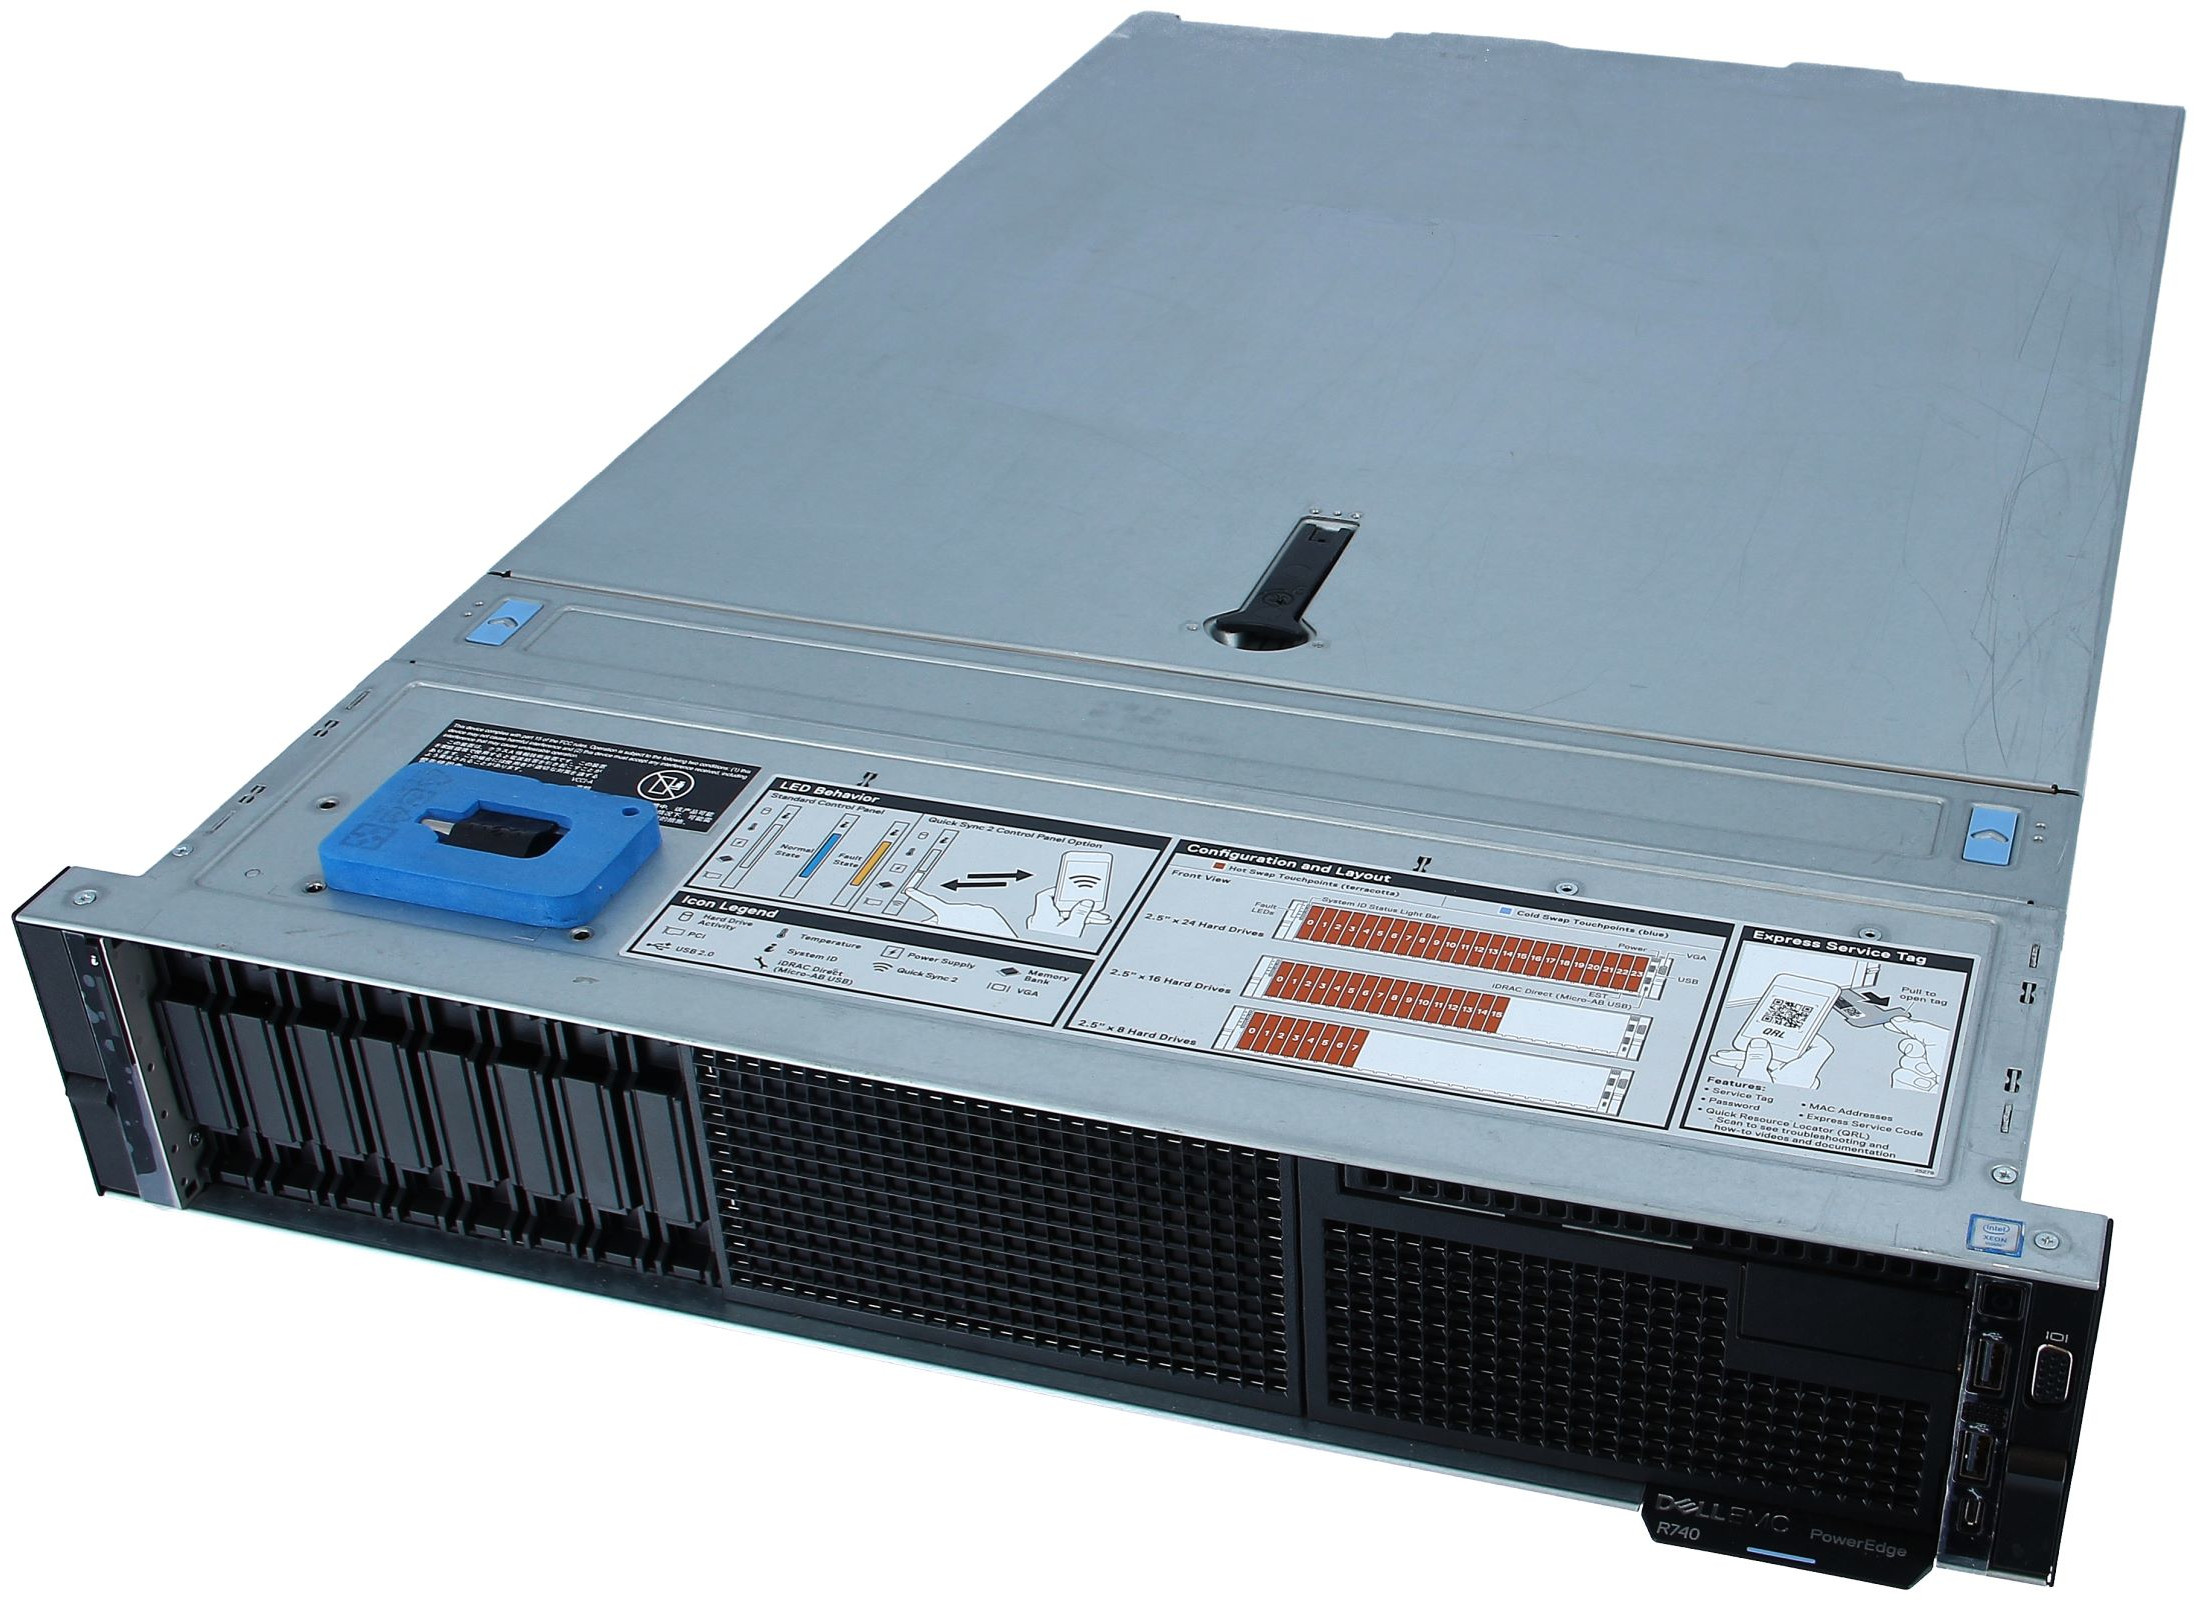
\includegraphics[width=3cm]{dell1}};
      \node at (3.5, -0.5) (cable) {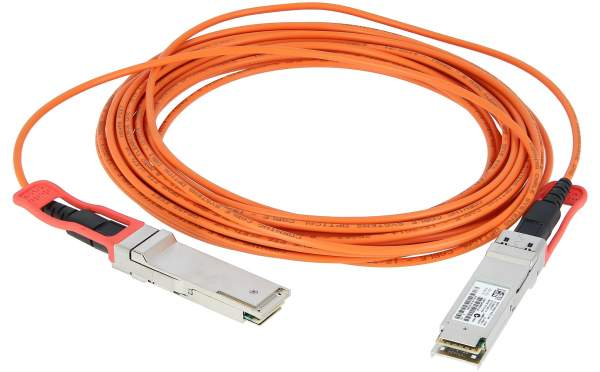
\includegraphics[width=2cm]{optical_fiber}};
      \node[inner sep=0] at (7, -0.5)   (Pj)    {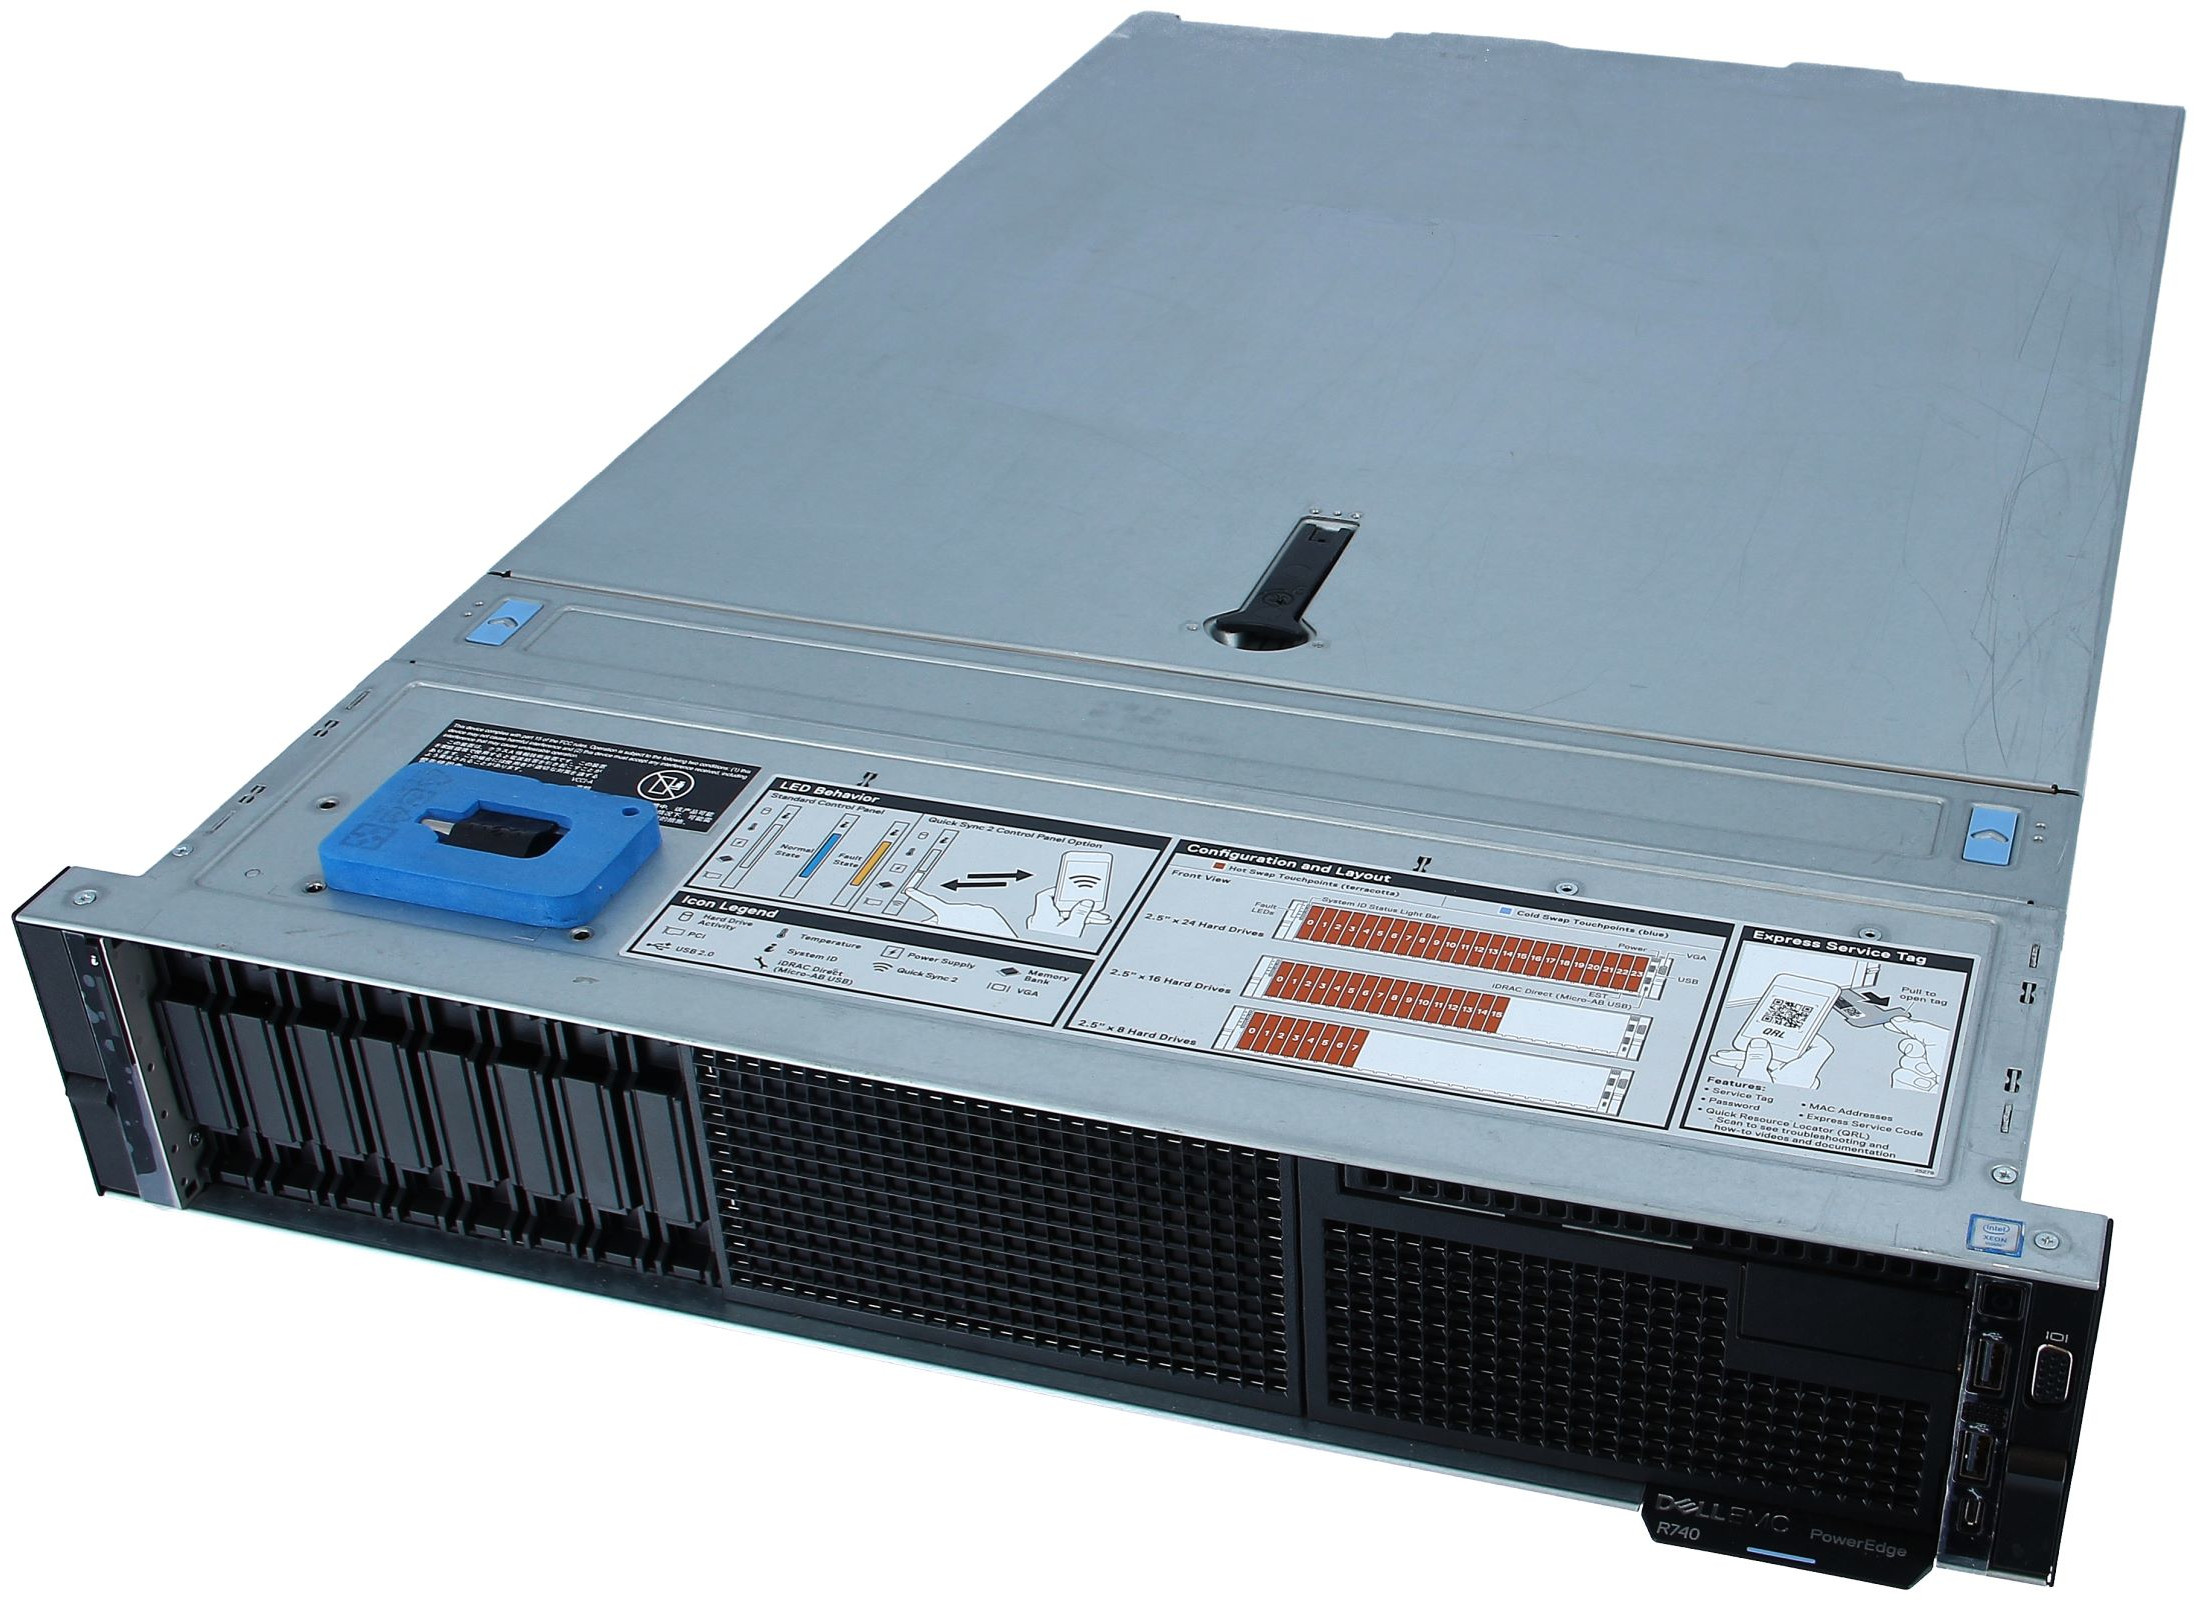
\includegraphics[width=3cm]{dell1}};
      \draw[<-, ultra thick] (Pi) -- (cable);
      \draw[->, ultra thick] (cable) -- (Pj);
    \end{scope}
  \end{tikzpicture}  
  
  \begin{block}{Sending a message along a network link}
    \begin{itemize}
    \item Reasonable to assume \alert{$T = \alpha + n \times \beta$}, where
      \begin{itemize}
      \item $n =$ message size (bits)
      \item $\alpha =$ \alert{latency} (s)
        \begin{itemize}
        \item MPI layer, OS, NICs, Switches, ...
        \end{itemize}
      \item $\beta = 1 / $ \alert{bandwidth} (s / bit).
      \end{itemize}

      \medskip

    \item Assumption: \alert{full-duplex}
      \begin{itemize}
      \item NICs can send \& receive at the same time
      \end{itemize}
    \end{itemize}
  \end{block}
\end{frame}

%%%%%%%%%%%%%%%%%%%%%%%%%%%%%%%%%%%%%%%%%%%%%%%%%%%%%%%%%%%%%%%%%%%%%%%%%%%

\begin{frame}
  \frametitle{Latency VS Bandwidth}
  
\footnotesize 
\begin{tabular}{|c|c|l|r|r|r|}
  \hline
  Cluster   &  Year & Interconnect & $1/\beta$ & $\alpha$ ($\mu$s) & $n\beta = \alpha$ \\
  \hline
  \hline
  PPTI      &  20?? & \phantom{00}1Gbit ethernet &    64MB/s & 50.0   & 3.2K \\
  sagitaire &  2006 & \phantom{00}1Gbit ethernet   &   116MB/s & 65.0 & 7.5K \\
  taurus    &  2012 & \phantom{0}10Gbit ethernet   &  1156MB/s & 25.9 & 30K  \\
  gros      &  2019 & \phantom{0}25Gbit ethernet   &  2480MB/s & 8.9  & 22K  \\
  \hline
  grcinq    &  2013 & \phantom{0}56Gbit InfiniBand &  2488MB/s & 1.2 & 3K    \\
  grimoire  &  2016 & \phantom{0}56Gbit InfiniBand &  4248MB/s & 1.1 & 4.6K  \\
  drac      &  2015 & 100Gbit InfiniBand        &  7760MB/s & 1.7    & 13K   \\
  \hline
  grvingt   &  2018 & 100Gbit OmniPath             & 12100MB/s & 0.9 & 11K   \\
  \hline
\end{tabular}

\end{frame}

%%%%%%%%%%%%%%%%%%%%%%%%%%%%%%%%%%%%%%%%%%%%%%%%%%%%%%%%%%%%%%%%%%%%%%%%%%

\subsection{Broadcast}

\begin{frame}
  \frametitle{Broadcast}

  \begin{center}
    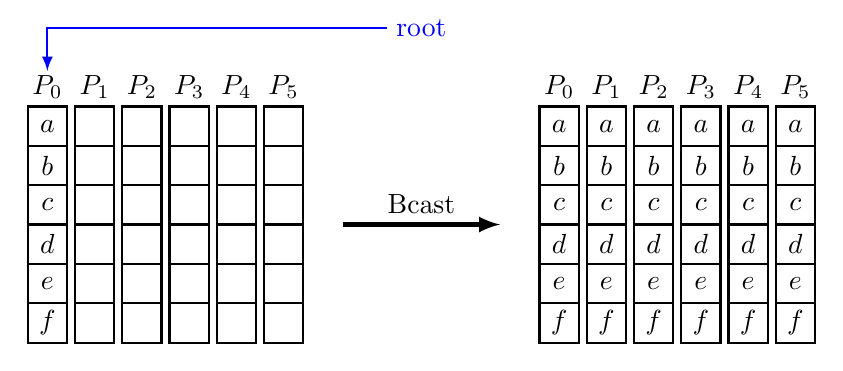
\begin{tikzpicture}[scale=0.5, >=latex]
      \path[use as bounding box] (0, 0) rectangle (20, 8);
  
      \node[blue] at (10, 8) (root) {root};
      \draw[thick, blue, ->] (root) -| (0.5, 6.9);
 
      \begin{scope}
        \foreach \i in {0,1,...,5} {
          \draw[thick] (1.2*\i, 0) rectangle +(1, 6);
          \foreach \j in {1,...,5} {
            \draw[thick] (1.2*\i, \j) -- +(1, 0);
          }
          \node at (1.2*\i + 0.5, 6.5) {$P_\i$};
        }
        \node at (0.5,  5.5) {$a$};
        \node at (0.5,  4.5) {$b$};
        \node at (0.5,  3.5) {$c$};
        \node at (0.5,  2.5) {$d$};
        \node at (0.5,  1.5) {$e$};
        \node at (0.5,  0.5) {$f$};
      \end{scope}
      
      \draw[ultra thick,->] (8, 3) -- node[above] {Bcast} (12, 3);
      
      \begin{scope}[xshift=13cm]
        \foreach \i in {0,1,...,5} {
          \draw[thick] (1.2*\i, 0) rectangle +(1, 6);
          \foreach \j in {1,...,5} {
            \draw[thick] (1.2*\i, \j) -- +(1, 0);
          }
          \node at (1.2*\i + 0.5, 6.5) {$P_\i$};
          \node at (1.2*\i + 0.5,  5.5) {$a$};
          \node at (1.2*\i + 0.5,  4.5) {$b$};
          \node at (1.2*\i + 0.5,  3.5) {$c$};
          \node at (1.2*\i + 0.5,  2.5) {$d$};
          \node at (1.2*\i + 0.5,  1.5) {$e$};
          \node at (1.2*\i + 0.5,  0.5) {$f$};
        }
      \end{scope}
    \end{tikzpicture}
  \end{center}

  %\vspace{-3ex}
  
  \begin{alertblock}{Lower bound}
    \begin{enumerate}
    \item $n$ elements exit from the {\color{blue} root}
      \begin{itemize}
      \item $T \geq n \beta$ \hfill (``bandwidth term'')
      \end{itemize}
    \item Reach everybody (``\emph{disease propagation}'')
      \begin{itemize}
      \item $\lceil \log_2 p \rceil$ successive messages \hfill (``latency term'')
      \end{itemize}
    \item[$\Longrightarrow$] $T \geq \lceil \log_2 p \rceil \alpha + n \beta$
    \end{enumerate}
  \end{alertblock}
\end{frame}

%%%%%%%%%%%%%%%%%%%%%%%%%%%%%%%%%%%%%%%%%%%%%%%%%%%%%%%%%%%%%%%%%%%%%%%%%%%%%%

\begin{frame}
  \frametitle{Naive Broadcast With Linear Network}
  
  \begin{center}
    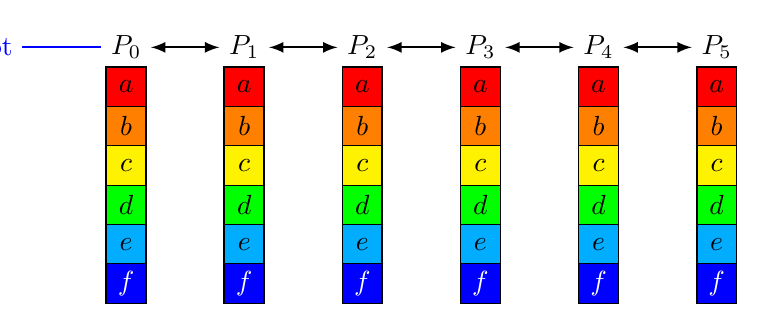
\begin{tikzpicture}[scale=0.5, >=latex]
      \path[use as bounding box] (-2, 0) rectangle (16, 7);
        
      %%%%%%%%%%%% Scatter / Gather
      \foreach \i in {0,1,...,5} {
        \draw[thick] (3*\i, 0) rectangle +(1, 6);
        \foreach \j in {1,...,5} {
          \draw[thick] (3*\i, \j) -- +(1, 0);
        }
        \node at (3*\i + 0.5, 6.5) (P\i) {$P_\i$};
      }

      \foreach \i in {1, 2, ..., 6} {
        \filldraw<\i->[fill=red]    (3*\i - 3, 5) rectangle node {$a$}  +(1,1);
        \filldraw<\i->[fill=orange] (3*\i - 3, 4) rectangle node {$b$} +(1,1);
        \filldraw<\i->[fill=yellow] (3*\i - 3, 3) rectangle node {$c$} +(1,1);
        \filldraw<\i->[fill=green]  (3*\i - 3, 2) rectangle node {$d$} +(1,1);
        \filldraw<\i->[fill=cyan]   (3*\i - 3, 1) rectangle node {$e$} +(1,1);
        \filldraw<\i->[fill=blue]   (3*\i - 3, 0) rectangle node[white] {$f$} +(1,1);
      }
      
      \draw[thick] (P0) edge[<->] (P1);
      \draw[thick] (P1) edge[<->] (P2);
      \draw[thick] (P2) edge[<->] (P3);
      \draw[thick] (P3) edge[<->] (P4);
      \draw[thick] (P4) edge[<->] (P5);

      \node[blue,left=of P0] (root) {root};
      \draw[thick, blue] (root) edge (P0);
    \end{tikzpicture}
  \end{center}

  \onslide<7->{
  \begin{block}{Summary}
    \begin{itemize}
    \item $p-1$ successive messages of size $n$
    \end{itemize}
  \end{block}

  \[
    T = \alert{(p-1)}\alpha + \alert{(p-1)} n \beta
  \]
  }
\end{frame}

%%%%%%%%%%%%%%%%%%%%%%%%%%%%%%%%%%%%%%%%%%%%%%%%%%%%%%%%%%%%%%%%%%%%%%%%%%%

\begin{frame}
  \frametitle{Pipelined Broadcast With Linear Network}
  
  \begin{center}
    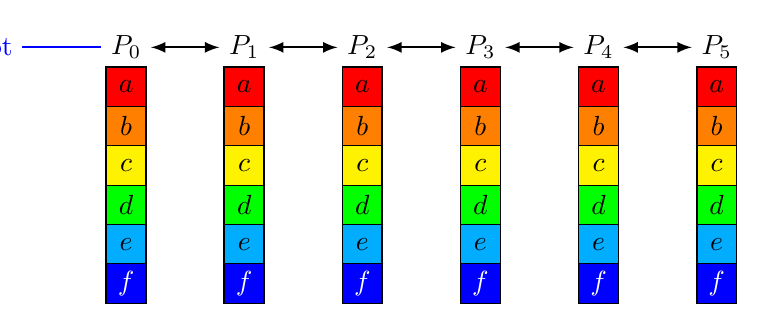
\begin{tikzpicture}[scale=0.5, >=latex]
      \path[use as bounding box] (-2, 0) rectangle (16, 7);
      %%%%%%%%%%%% Bcast pipeline
      \foreach \i in {0,1,...,5} {
        \draw[thick] (3*\i, 0) rectangle +(1, 6);
        \foreach \j in {1,...,5} {
          \draw[thick] (3*\i, \j) -- +(1, 0);
        }
        \node at (3*\i + 0.5, 6.5) (P\i) {$P_\i$};
      }
      \draw[thick] (P0) edge[<->] (P1);
      \draw[thick] (P1) edge[<->] (P2);
      \draw[thick] (P2) edge[<->] (P3);
      \draw[thick] (P3) edge[<->] (P4);
      \draw[thick] (P4) edge[<->] (P5);

      \node[blue,left=of P0] (root) {root};
      \draw[thick, blue] (root) edge (P0);

      \filldraw[fill=red]    (0, 5) rectangle node {$a$}  +(1,1);
      \filldraw[fill=orange] (0, 4) rectangle node {$b$} +(1,1);
      \filldraw[fill=yellow] (0, 3) rectangle node {$c$} +(1,1);
      \filldraw[fill=green]  (0, 2) rectangle node {$d$} +(1,1);
      \filldraw[fill=cyan]   (0, 1) rectangle node {$e$} +(1,1);
      \filldraw[fill=blue]   (0, 0) rectangle node[white] {$f$} +(1,1);

      
      \foreach \i in {2, ..., 6} {
        \filldraw<\i->[fill=red]    (3*\i - 3, 5) rectangle node {$a$}  +(1,1);
      }
      \foreach \i in {3, ..., 7} {
        \filldraw<\i->[fill=orange] (3*\i - 6, 4) rectangle node {$b$} +(1,1);
      }
      \foreach \i in {4, ..., 8} {
        \filldraw<\i->[fill=yellow] (3*\i - 9, 3) rectangle node {$c$} +(1,1);
      }
      \foreach \i in {5, ..., 9} {
        \filldraw<\i->[fill=green]  (3*\i - 12, 2) rectangle node {$d$} +(1,1);
      }
      \foreach \i in {6, ..., 10} {
        \filldraw<\i->[fill=cyan]   (3*\i - 15, 1) rectangle node {$e$} +(1,1);
      }
      \foreach \i in {7, ..., 11} {
        \filldraw<\i->[fill=blue]   (3*\i - 18, 0) rectangle node[white] {$f$} +(1,1);
      }
    \end{tikzpicture}
  \end{center}

  \onslide<11->{
  \begin{block}{\vspace*{-3ex}}
    \begin{itemize}
    \item Pipelining: $k$ ``phases''
      \begin{itemize}
      \item Naive broadcasts of size $n/k$
      \end{itemize}
    \item $k+p-2$ successive messages of size $n/k$
    \end{itemize}
  \end{block}
  \[
    T = \alert{(k + p-2)}\alpha + \alert{\left(1 + \frac{p-2}{k}\right)} n \beta
  \]
  $k = p-2$ makes sense; best choice: $k = \sqrt{(p - 2)\beta n/\alpha }$)
  }
\end{frame}


%%%%%%%%%%%%%%%%%%%%%%%%%%%%%%%%%%%%%%%%%%%%%%%%%%%%%%%%%%%%%%%%%%%%%%%%%%%%

\begin{frame}<1>[label=bcast_2D_torus]
  \frametitle{Naive Broadcast With 2D Torus Network}

  \begin{center}
    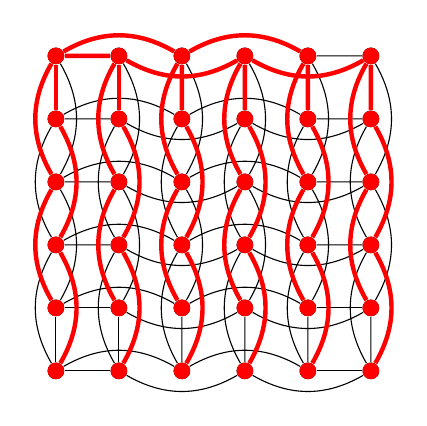
\begin{tikzpicture}[scale=0.8]
      
      \foreach \i in {0, 1, ..., 5} {
        \foreach \j in {0, 1, ..., 5}{
          \node[fill=black, shape=circle, inner sep=0.75mm] at (\i, \j) (n\i\j) {};
        }
      }
      \foreach \i in {0, 1, ..., 5}
      {
        \draw (n0\i) edge[bend left] (n2\i);
        \draw (n2\i) edge[bend left] (n4\i);
        \draw (n4\i) edge            (n5\i);
        \draw (n5\i) edge[bend left] (n3\i);
        \draw (n3\i) edge[bend left] (n1\i);
        \draw (n1\i) edge            (n0\i);
  
        \draw (n\i0) edge[bend left] (n\i2);
        \draw (n\i2) edge[bend left] (n\i4);
        \draw (n\i4) edge            (n\i5);
        \draw (n\i5) edge[bend left] (n\i3);
        \draw (n\i3) edge[bend left] (n\i1);
        \draw (n\i1) edge            (n\i0);
      }

      % top row
      \node<1->[fill=red, shape=circle, inner sep=0.75mm] at (0, 5) {};
      \node<2->[fill=red, shape=circle, inner sep=0.75mm] at (1, 5) {};
      \node<3->[fill=red, shape=circle, inner sep=0.75mm] at (2, 5) {};
      \node<3->[fill=red, shape=circle, inner sep=0.75mm] at (3, 5) {};
      \node<4->[fill=red, shape=circle, inner sep=0.75mm] at (4, 5) {};
      \node<4->[fill=red, shape=circle, inner sep=0.75mm] at (5, 5) {};

      \draw<2>[red,ultra thick] (n05) edge (n15);
      \draw<3>[red,ultra thick] (n05) edge[bend left] (n25);
      \draw<3>[red,ultra thick] (n15) edge[bend right] (n35);
      \draw<4>[red,ultra thick] (n25) edge[bend left] (n45);
      \draw<4>[red,ultra thick] (n35) edge[bend right] (n55);

      % x=0
      \node<4->[fill=red, shape=circle, inner sep=0.75mm] at (0, 4) {};
      \node<5->[fill=red, shape=circle, inner sep=0.75mm] at (0, 2) {};
      \node<5->[fill=red, shape=circle, inner sep=0.75mm] at (0, 3) {};
      \node<6->[fill=red, shape=circle, inner sep=0.75mm] at (0, 0) {};
      \node<6->[fill=red, shape=circle, inner sep=0.75mm] at (0, 1) {};

      \draw<4>[red,ultra thick] (n05) edge (n04);
      \draw<5>[red,ultra thick] (n05) edge[bend right] (n03);
      \draw<5>[red,ultra thick] (n04) edge[bend left] (n02);
      \draw<6>[red,ultra thick] (n03) edge[bend right] (n01);
      \draw<6>[red,ultra thick] (n02) edge[bend left] (n00);

      % x=1
      \node<4->[fill=red, shape=circle, inner sep=0.75mm] at (1, 4) {};
      \node<5->[fill=red, shape=circle, inner sep=0.75mm] at (1, 2) {};
      \node<5->[fill=red, shape=circle, inner sep=0.75mm] at (1, 3) {};
      \node<6->[fill=red, shape=circle, inner sep=0.75mm] at (1, 0) {};
      \node<6->[fill=red, shape=circle, inner sep=0.75mm] at (1, 1) {};

      \draw<4>[red,ultra thick] (n15) edge             (n14);
      \draw<5>[red,ultra thick] (n15) edge[bend right] (n13);
      \draw<5>[red,ultra thick] (n14) edge[bend left]  (n12);
      \draw<6>[red,ultra thick] (n13) edge[bend right] (n11);
      \draw<6>[red,ultra thick] (n12) edge[bend left]  (n10);
      
      % x=2
      \node<5->[fill=red, shape=circle, inner sep=0.75mm] at (2, 4) {};
      \node<6->[fill=red, shape=circle, inner sep=0.75mm] at (2, 2) {};
      \node<6->[fill=red, shape=circle, inner sep=0.75mm] at (2, 3) {};
      \node<7->[fill=red, shape=circle, inner sep=0.75mm] at (2, 0) {};
      \node<7->[fill=red, shape=circle, inner sep=0.75mm] at (2, 1) {};

      \draw<5>[red,ultra thick] (n25) edge             (n24);
      \draw<6>[red,ultra thick] (n25) edge[bend right] (n23);
      \draw<6>[red,ultra thick] (n24) edge[bend left]  (n22);
      \draw<7>[red,ultra thick] (n23) edge[bend right] (n21);
      \draw<7>[red,ultra thick] (n22) edge[bend left]  (n20);

      % x=3
      \node<6->[fill=red, shape=circle, inner sep=0.75mm] at (3, 4) {};
      \node<7->[fill=red, shape=circle, inner sep=0.75mm] at (3, 2) {};
      \node<7->[fill=red, shape=circle, inner sep=0.75mm] at (3, 3) {};
      \node<8->[fill=red, shape=circle, inner sep=0.75mm] at (3, 0) {};
      \node<8->[fill=red, shape=circle, inner sep=0.75mm] at (3, 1) {};

      \draw<6>[red,ultra thick] (n35) edge             (n34);
      \draw<7>[red,ultra thick] (n35) edge[bend right] (n33);
      \draw<7>[red,ultra thick] (n34) edge[bend left]  (n32);
      \draw<8>[red,ultra thick] (n33) edge[bend right] (n31);
      \draw<8>[red,ultra thick] (n32) edge[bend left]  (n30);

      % x=4
      \node<7->[fill=red, shape=circle, inner sep=0.75mm] at (4, 4) {};
      \node<8->[fill=red, shape=circle, inner sep=0.75mm] at (4, 2) {};
      \node<8->[fill=red, shape=circle, inner sep=0.75mm] at (4, 3) {};
      \node<9->[fill=red, shape=circle, inner sep=0.75mm] at (4, 0) {};
      \node<9->[fill=red, shape=circle, inner sep=0.75mm] at (4, 1) {};

      \draw<7>[red,ultra thick] (n45) edge             (n44);
      \draw<8>[red,ultra thick] (n45) edge[bend right] (n43);
      \draw<8>[red,ultra thick] (n44) edge[bend left]  (n42);
      \draw<9>[red,ultra thick] (n43) edge[bend right] (n41);
      \draw<9>[red,ultra thick] (n42) edge[bend left]  (n40);

      % x=5
      \node<8->[fill=red, shape=circle, inner sep=0.75mm] at  (5, 4) {};
      \node<9->[fill=red, shape=circle, inner sep=0.75mm] at  (5, 2) {};
      \node<9->[fill=red, shape=circle, inner sep=0.75mm] at  (5, 3) {};
      \node<10->[fill=red, shape=circle, inner sep=0.75mm] at (5, 0) {};
      \node<10->[fill=red, shape=circle, inner sep=0.75mm] at (5, 1) {};

      \draw<8>[red,ultra thick]  (n55) edge             (n54);
      \draw<9>[red,ultra thick]  (n55) edge[bend right] (n53);
      \draw<9>[red,ultra thick]  (n54) edge[bend left]  (n52);
      \draw<10>[red,ultra thick] (n53) edge[bend right] (n51);
      \draw<10>[red,ultra thick] (n52) edge[bend left]  (n50);

    \end{tikzpicture}        
  \end{center}
  \onslide<10->{
  \begin{itemize}
  \item $2\sqrt{p}$ successive messages of size $n$
  \end{itemize}
  \[
    T = \alert{2\sqrt{p}} \alpha + \alert{2 \sqrt{p}} n\beta 
  \]
  }
\end{frame}

\begin{frame}
  \frametitle{Naive Broadcast With 2D Torus Network}

  \begin{center}
    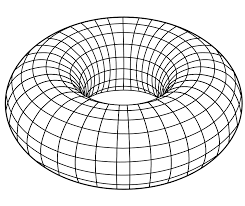
\includegraphics[width=6cm]{torus.png}
  \end{center}
\end{frame}

\againframe<2->{bcast_2D_torus}

%%%%%%%%%%%%%%%%%%%%%%%%%%%%%%%%%%%%%%%%%%%%%%%%%%%%%%%%%%%%%%%%%%%%%%%%%%%%

\subsection{Gather/scatter}

\begin{frame}
\frametitle{Scatter/Gather: Lower Bound}

\begin{center}
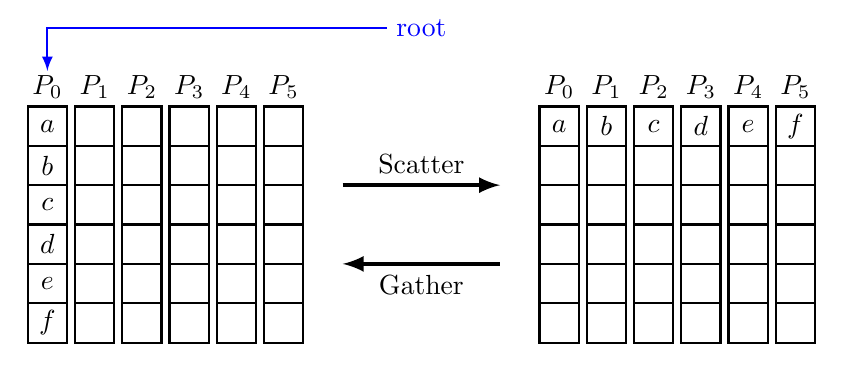
\begin{tikzpicture}[scale=0.5, >=latex]
  \path[use as bounding box] (0, 0) rectangle (20, 8);
  
  \node[blue] at (10, 8) (root) {root};
  \draw[thick, blue, ->] (root) -| (0.5, 6.9);
 
%%%%%%%%%%%% Scatter / Gather
  \begin{scope}
    \foreach \i in {0,1,...,5} {
      \draw[thick] (1.2*\i, 0) rectangle +(1, 6);
      \foreach \j in {1,...,5} {
        \draw[thick] (1.2*\i, \j) -- +(1, 0);
      }
      \node at (1.2*\i + 0.5, 6.5) {$P_\i$};
    }
  \node at (0.5,  5.5) {$a$};
  \node at (0.5,  4.5) {$b$};
  \node at (0.5,  3.5) {$c$};
  \node at (0.5,  2.5) {$d$};
  \node at (0.5,  1.5) {$e$};
  \node at (0.5,  0.5) {$f$};
  \end{scope}
  
\draw[ultra thick,->] (8, 4) -- node[above] {Scatter} (12, 4);
\draw[ultra thick,<-] (8, 2) -- node[below] {Gather} (12, 2);

\begin{scope}[xshift=13cm]
   \foreach \i in {0,1,...,5} {
      \draw[thick] (1.2*\i, 0) rectangle +(1, 6);
      \foreach \j in {1,...,5} {
        \draw[thick] (1.2*\i, \j) -- +(1, 0);
      }
      \node at (1.2*\i + 0.5, 6.5) {$P_\i$};
    }
    \node at (0.5,  5.5) {$a$};
    \node at (1.7,  5.5) {$b$};
    \node at (2.9,  5.5) {$c$};
    \node at (4.1,  5.5) {$d$};
    \node at (5.3,  5.5) {$e$};
    \node at (6.5,  5.5) {$f$};
      \end{scope}
    \end{tikzpicture}
  \end{center}

  \vspace{-3ex}
  
  \begin{alertblock}{\vspace*{-3ex}}
    \begin{enumerate}
    \item $(p-1) \frac{n}{p}$ elements exit from (resp. enter into) {\color{blue} root}
      \begin{itemize}
      \item $T \geq (p-1) \frac{n}{p} \beta$ \hfill (``bandwidth term'')
      \end{itemize}
    \item Reach everybody (``\emph{disease propagation}'')
      \begin{itemize}
      \item $\lceil \log_2 p \rceil$ successive messages \hfill (``latency term'')
      \end{itemize}
    \end{enumerate}
  \end{alertblock}
  
  \[
    \Longrightarrow T \geq \lceil \log_2 p \rceil \alpha + (p-1) \frac{n}{p} \beta
  \]
\end{frame}

%%%%%%%%%%%%%%%%%%%%%%%%%%%%%%%%%%%%%%%%%%%%%%%%%%%%%%%%%%%%%%%%%%%%%%%%%%%%%%

\begin{frame}
  \frametitle{Scatter With Linear Network}

  \begin{center}
    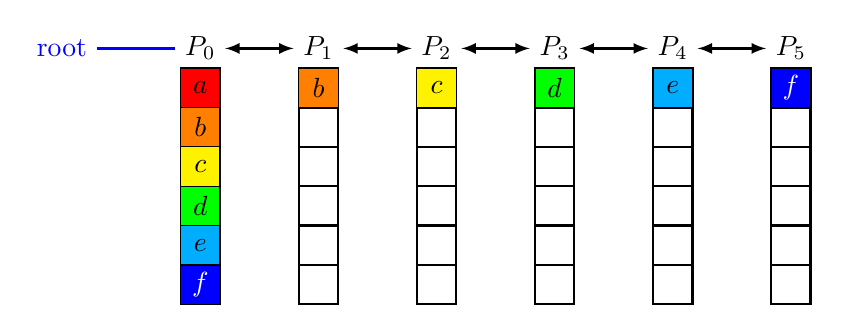
\begin{tikzpicture}[scale=0.5, >=latex]
        
      %%%%%%%%%%%% Scatter / Gather
      \foreach \i in {0,1,...,5} {
        \draw[thick] (3*\i, 0) rectangle +(1, 6);
        \foreach \j in {1,...,5} {
          \draw[thick] (3*\i, \j) -- +(1, 0);
        }
        \node at (3*\i + 0.5, 6.5) (P\i) {$P_\i$};
      }
      
      \filldraw[fill=red]    (0, 5) rectangle  +(1,1);
      \filldraw<1-5>[fill=orange] (0, 4) rectangle  +(1,1);
      \filldraw<1-4>[fill=yellow] (0, 3) rectangle  +(1,1);
      \filldraw<1-3>[fill=green]  (0, 2) rectangle  +(1,1);
      \filldraw<1-2>[fill=cyan]   (0, 1) rectangle  +(1,1);
      \filldraw<1>[fill=blue]   (0, 0) rectangle  +(1,1);
      
      \node at (0.5,  5.5) {$a$};
      \node<1-5> at (0.5,  4.5) {$b$};
      \node<1-4> at (0.5,  3.5) {$c$};
      \node<1-3> at (0.5,  2.5) {$d$};
      \node<1-2> at (0.5,  1.5) {$e$};
      \node<1>[text=white] at (0.5,  0.5) {$f$};

      \draw[thick] (P0) edge[<->] (P1);
      \draw[thick] (P1) edge[<->] (P2);
      \draw[thick] (P2) edge[<->] (P3);
      \draw[thick] (P3) edge[<->] (P4);
      \draw[thick] (P4) edge[<->] (P5);

      \node[blue,left=of P0] (root) {root};
      \draw[thick, blue] (root) edge (P0);

      % t=2
      \filldraw<2>[fill=blue]   (3, 5) rectangle  +(1,1);
      \node<2>[text=white] at (3.5,  5.5) {$f$};

      % t=3
      \filldraw<3>[fill=cyan]   (3, 5) rectangle  +(1,1);
      \node<3> at (3.5,  5.5) {$e$};
      \filldraw<3>[fill=blue]   (6, 5) rectangle  +(1,1);
      \node<3>[text=white] at (6.5,  5.5) {$f$};

      % t=4
      \filldraw<4>[fill=green]   (3, 5) rectangle  +(1,1);
      \node<4> at (3.5,  5.5) {$d$};
      \filldraw<4>[fill=cyan]   (6, 5) rectangle  +(1,1);
      \node<4> at (6.5,  5.5) {$e$};      
      \filldraw<4>[fill=blue]   (9, 5) rectangle  +(1,1);
      \node<4>[text=white] at (9.5,  5.5) {$f$};

      % t=5
      \filldraw<5>[fill=yellow]   (3, 5) rectangle  +(1,1);
      \node<5> at (3.5,  5.5) {$c$};
      \filldraw<5>[fill=green]   (6, 5) rectangle  +(1,1);
      \node<5> at (6.5,  5.5) {$d$};
      \filldraw<5>[fill=cyan]   (9, 5) rectangle  +(1,1);
      \node<5> at (9.5,  5.5) {$e$};      
      \filldraw<5>[fill=blue]   (12, 5) rectangle  +(1,1);
      \node<5>[text=white] at (12.5,  5.5) {$f$};

      % t=6
      \filldraw<6>[fill=orange]   (3, 5) rectangle  +(1,1);
      \node<6> at (3.5,  5.5) {$b$};
      \filldraw<6>[fill=yellow]   (6, 5) rectangle  +(1,1);
      \node<6> at (6.5,  5.5) {$c$};
      \filldraw<6>[fill=green]   (9, 5) rectangle  +(1,1);
      \node<6> at (9.5,  5.5) {$d$};
      \filldraw<6>[fill=cyan]   (12, 5) rectangle  +(1,1);
      \node<6> at (12.5,  5.5) {$e$};      
      \filldraw<6>[fill=blue]   (15, 5) rectangle  +(1,1);
      \node<6>[text=white] at (15.5,  5.5) {$f$};
    \end{tikzpicture}
  \end{center}

  \onslide<6->{
  \begin{block}{Summary}
    \begin{itemize}
    \item $p-1$ successive messages of size $n/p$
    \item Parallel communications (``pipeline'')
    \end{itemize}
  \end{block}

  \[
    T = \alert{(p-1)}\alpha + (p-1) \frac{n}{p} \beta
  \]
  }
\end{frame}

%%%%%%%%%%%%%%%%%%%%%%%%%%%%%%%%%%%%%%%%%%%%%%%%%%%%%%%%%%%%%%%%%
\subsection{Allgather}

\begin{frame}
\frametitle{Gather-to-All}

  \begin{center}
    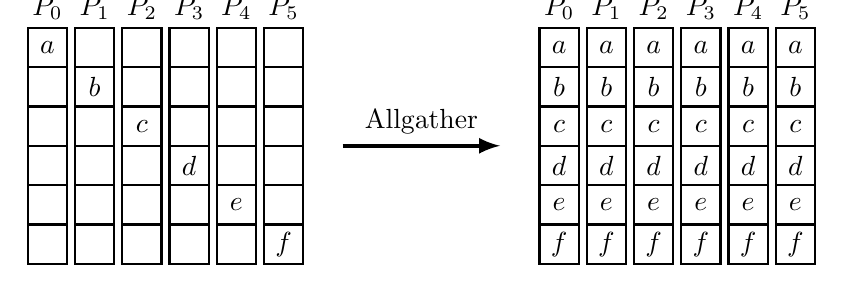
\begin{tikzpicture}[scale=0.5, >=latex]
      \path[use as bounding box] (0, 0) rectangle (20, 6);
      
      \begin{scope}
        \foreach \i in {0,1,...,5} {
          \draw[thick] (1.2*\i, 0) rectangle +(1, 6);
          \foreach \j in {1,...,5} {
            \draw[thick] (1.2*\i, \j) -- +(1, 0);
          }
          \node at (1.2*\i + 0.5, 6.5) {$P_\i$};
        }
        \node at (0.5,  5.5) {$a$};
        \node at (1.7,  4.5) {$b$};
        \node at (2.9,  3.5) {$c$};
        \node at (4.1,  2.5) {$d$};
        \node at (5.3,  1.5) {$e$};
        \node at (6.5,  0.5) {$f$};
      \end{scope}
      
      \draw[ultra thick,->] (8, 3) -- node[above] {Allgather} (12, 3);
      
      \begin{scope}[xshift=13cm]
        \foreach \i in {0,1,...,5} {
          \draw[thick] (1.2*\i, 0) rectangle +(1, 6);
          \foreach \j in {1,...,5} {
            \draw[thick] (1.2*\i, \j) -- +(1, 0);
          }
          \node at (1.2*\i + 0.5, 6.5) {$P_\i$};
          \node at (1.2*\i + 0.5,  5.5) {$a$};
          \node at (1.2*\i + 0.5,  4.5) {$b$};
          \node at (1.2*\i + 0.5,  3.5) {$c$};
          \node at (1.2*\i + 0.5,  2.5) {$d$};
          \node at (1.2*\i + 0.5,  1.5) {$e$};
          \node at (1.2*\i + 0.5,  0.5) {$f$};
        }
      \end{scope}
    \end{tikzpicture}
  \end{center}

    \vspace{-3ex}
  
  \begin{alertblock}{\vspace*{-3ex}}
    \begin{enumerate}
    \item $(p-1) \frac{n}{p}$ elements exit from each node
      \begin{itemize}
      \item $T \geq (p-1) \frac{n}{p} \beta$ \hfill (``bandwidth term'')
      \end{itemize}
    \item Reach everybody (``\emph{disease propagation}'')
      \begin{itemize}
      \item $\lceil \log_2 p \rceil$ successive messages \hfill (``latency term'')
      \end{itemize}
    \end{enumerate}
  \end{alertblock}
  \[
    \Longrightarrow T \geq \lceil \log_2 p \rceil \alpha + (p-1) \frac{n}{p} \beta
  \]
\end{frame}

%%%%%%%%%%%%%%%%%%%%%%%%%%%%%%%%%%%%%%%%%%%%%%%%%%%%%%%%%%%%%%%%%%%%%%%%%%%%%%%%

\begin{frame}[label=alg]
  \frametitle{Allgather on 1D Torus Network}
  \begin{center}
    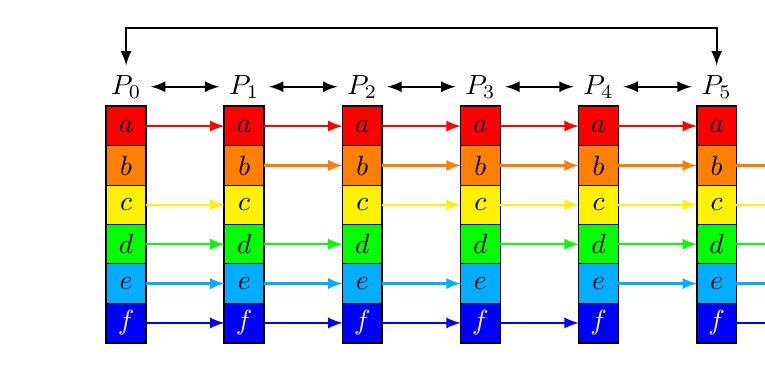
\begin{tikzpicture}[scale=0.5, >=latex]
      \path[use as bounding box] (-2, 0) rectangle (16, 8);

      \foreach \i in {0,1,...,5} {
        \draw[thick] (3*\i, 0) rectangle +(1, 6);
        \foreach \j in {1,...,5} {
          \draw[thick] (3*\i, \j) -- +(1, 0);
        }
        \node at (3*\i + 0.5, 6.5) (P\i) {$P_\i$};
      }
      \draw[thick] (P0) edge[<->] (P1);
      \draw[thick] (P1) edge[<->] (P2);
      \draw[thick] (P2) edge[<->] (P3);
      \draw[thick] (P3) edge[<->] (P4);
      \draw[thick] (P4) edge[<->] (P5);
      \draw[thick,<->] (P5) -- ++(0, 1.5) -| (P0);

      \foreach \t in {1, ..., 6} {
        \tikzmath{
          \i = mod(\t-1, 6);
          \j = mod(\t, 6);
          \k = mod(\t+1, 6);
          \l = mod(\t+2, 6);
          \m = mod(\t+3, 6);
          \n = mod(\t+4, 6);
        }
        \filldraw<\t->[fill=red]    (3*\i, 5) rectangle node {$a$}  +(1,1);
        \filldraw<\t->[fill=orange] (3*\j, 4) rectangle node {$b$} +(1,1);
        \filldraw<\t->[fill=yellow] (3*\k, 3) rectangle node {$c$} +(1,1);
        \filldraw<\t->[fill=green]  (3*\l, 2) rectangle node {$d$} +(1,1);
        \filldraw<\t->[fill=cyan]   (3*\m, 1) rectangle node {$e$} +(1,1);
        \filldraw<\t->[fill=blue]   (3*\n, 0) rectangle node[white] {$f$} +(1,1);

        \ifthenelse{\t < 6}{
          \draw<\t>[->, red, thick]    (3*\i + 1, 5.5) -- +(2, 0);
          \draw<\t>[->, orange, thick] (3*\j + 1, 4.5) -- +(2, 0);
          \draw<\t>[->, yellow, thick] (3*\k + 1, 3.5) -- +(2, 0);
          \draw<\t>[->, green, thick]  (3*\l + 1, 2.5) -- +(2, 0);
          \draw<\t>[->, cyan, thick]   (3*\m + 1, 1.5) -- +(2, 0);
          \draw<\t>[->, blue, thick]   (3*\n + 1, 0.5) -- +(2, 0);
        }{}
      }
    \end{tikzpicture}
  \end{center}

  
  \begin{block}<6->{\vspace*{-3ex}}
    \begin{itemize}
    \item Step 1: send you own data; step $i+1$: send what you just received
    \item $p-1$ successive messages of size $n/p$
    \end{itemize}
  \[
    T = \alert{(p-1)}\alpha + \left(\frac{p-1}{p}\right) n \beta
  \]
  \end{block}
 
\end{frame}


%%%%%%%%%%%%%%%%%%%%%%%%%%%%%%%%%%%%%%%%%%%%%%%%%%%%%%%%%%%%%%%%%%%%%%%%%%%%%%%%

\section{With generic Topologies}

%%%%%%%%%%%%%%%%%%%%%%%%%%%%%%%%%%%%%%%%%%%%%%%%%%%%%%%%%%%%%%%%%%%%%%%%%%%%%

\begin{frame}

  \vfill
  \large

  \begin{alertblock}{Performance of collective operations...}
    ... heavily affected by \textbf{network topology}
  \end{alertblock}

  \vfill

  \begin{block}{Topology}
    Bipartite graph with (NIC, Switch) nodes and link edges
  \end{block}

  \vfill
\end{frame}

%%%%%%%%%%%%%%%%%%%%%%%%%%%%%%%%%%%%%%%%%%%%%%%%%%%%%%%%%%%%%%%%%%%%%%%%%%%%%%

\begin{frame}
  \frametitle{How Long Does It Take to Communicate (redux)?}
  
  \begin{tikzpicture}
    \begin{scope}[xshift=0cm]
      \node[inner sep=0] at (0, -0.5)   (Pi)    {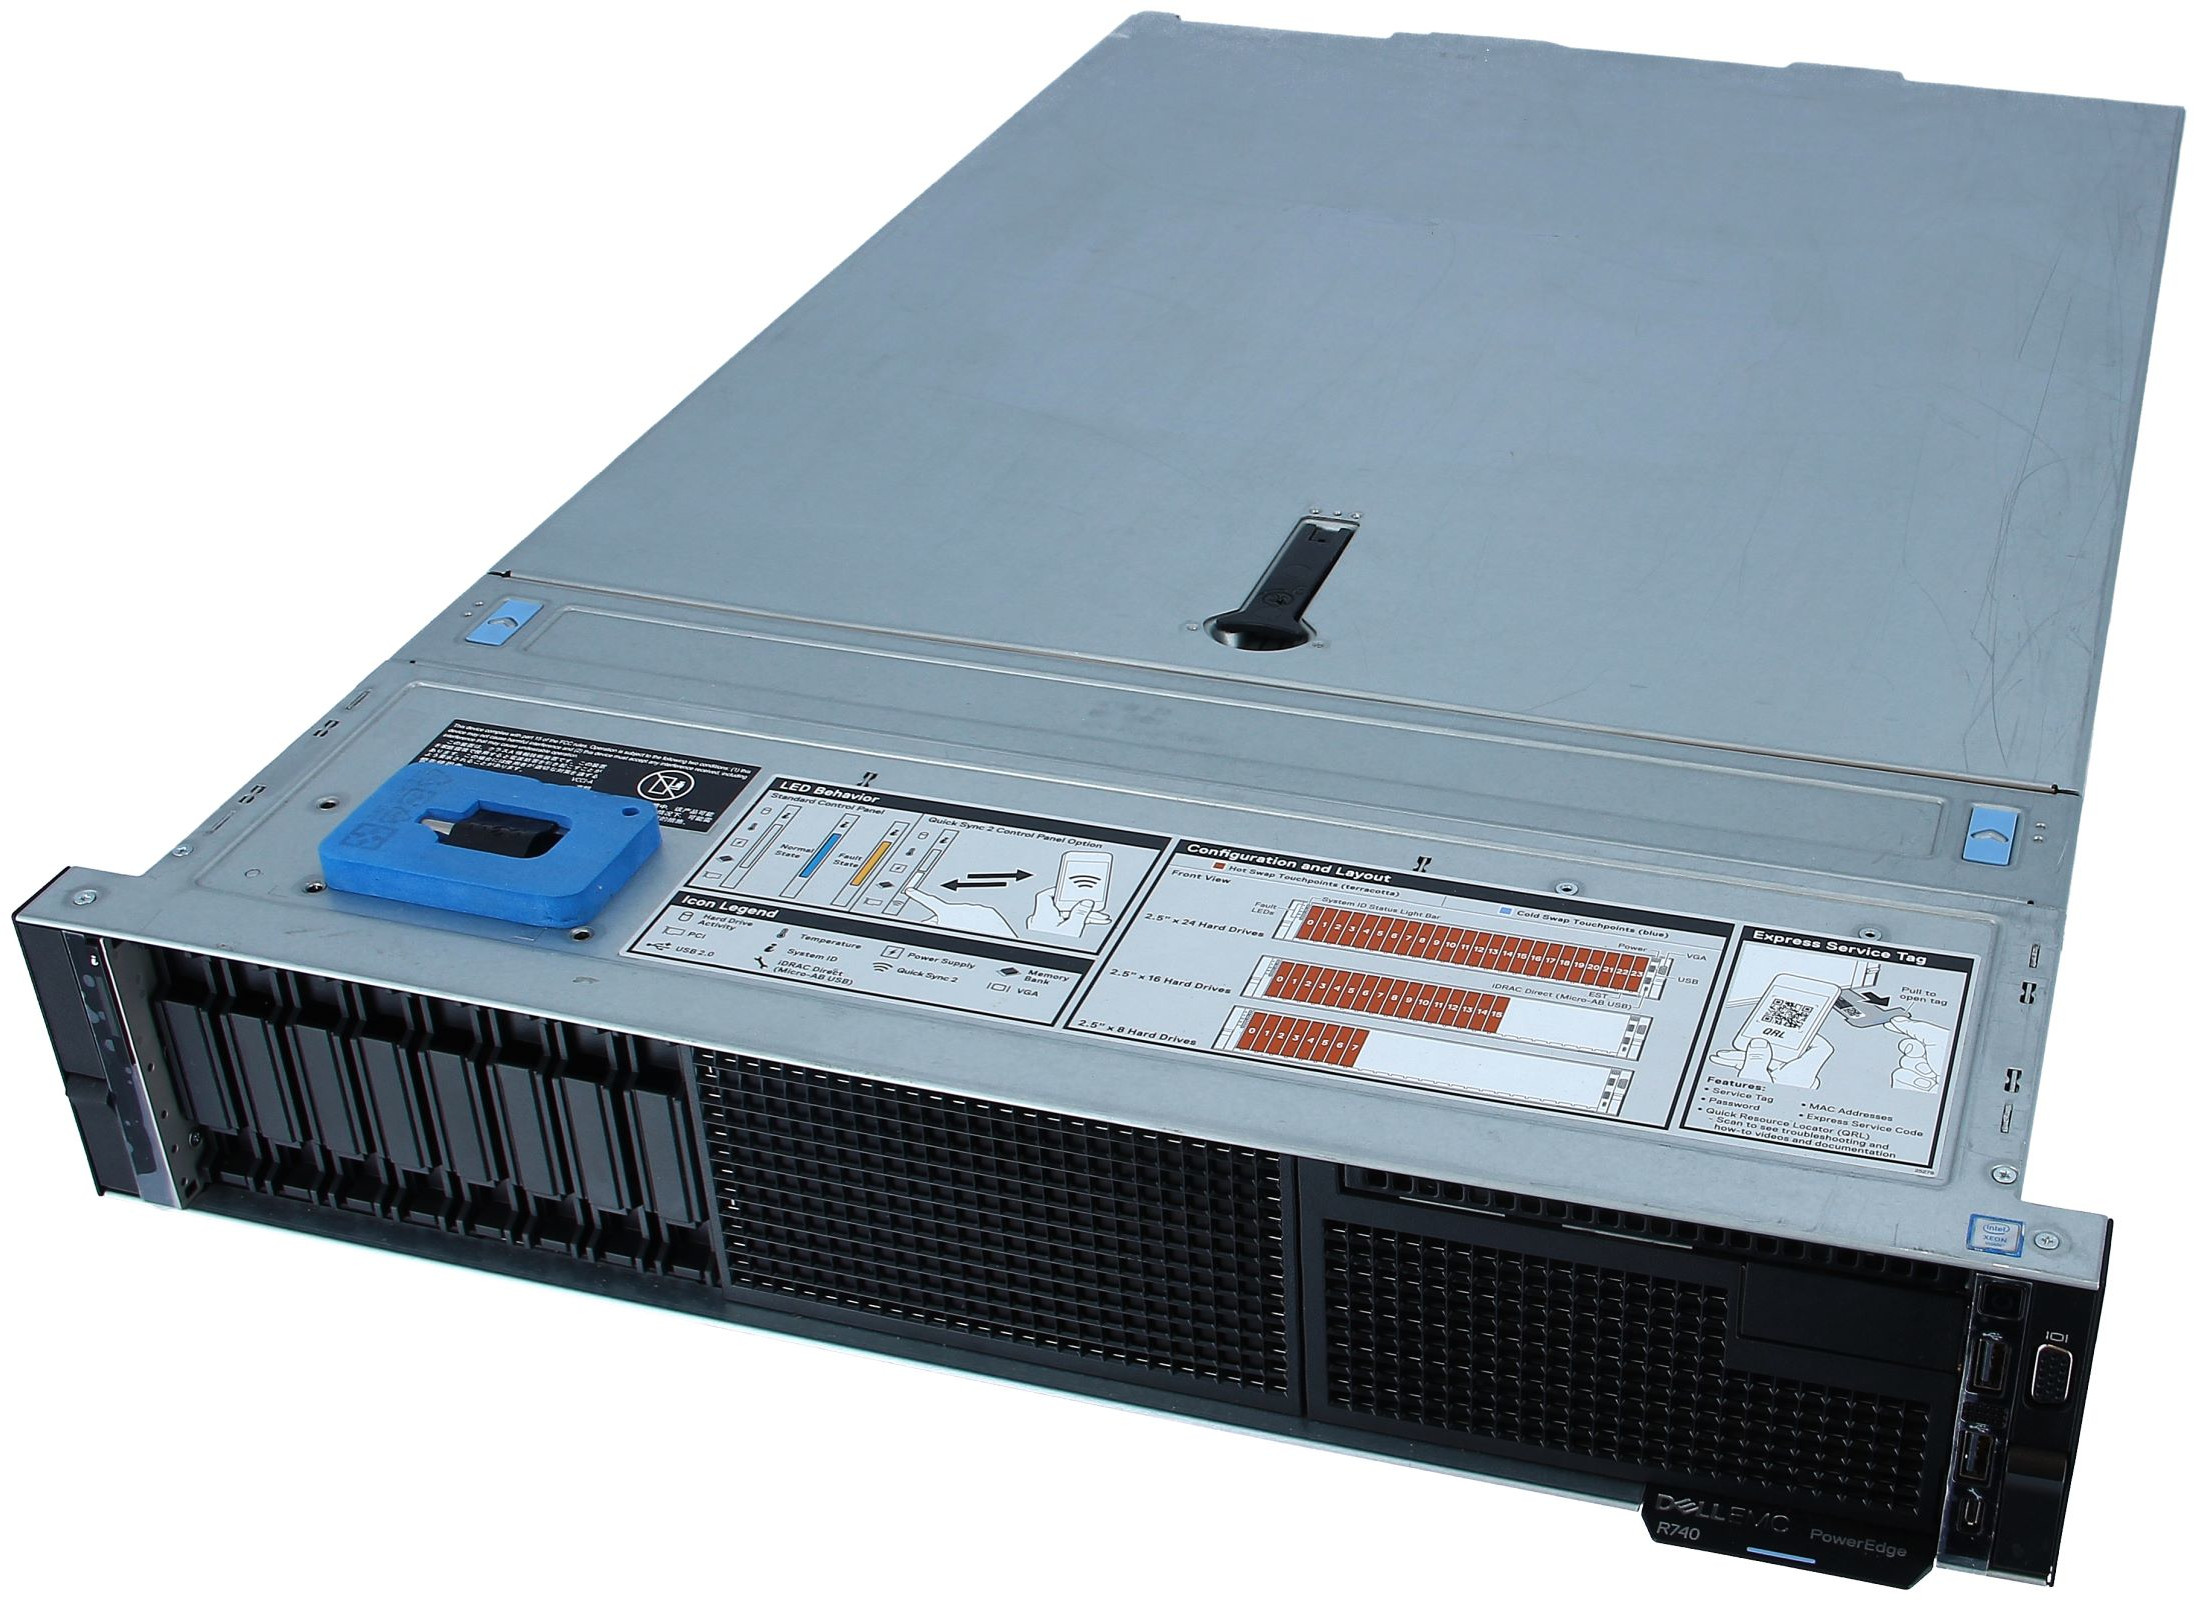
\includegraphics[width=3cm]{dell1}};
      \node at (3.5, -0.5) (cable) {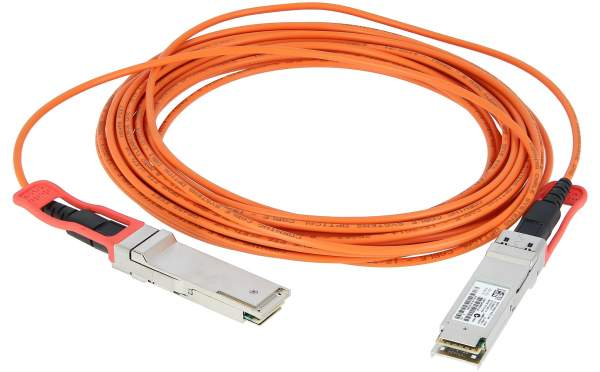
\includegraphics[width=2cm]{optical_fiber}};
      \node[inner sep=0] at (7, -0.5)   (Pj)    {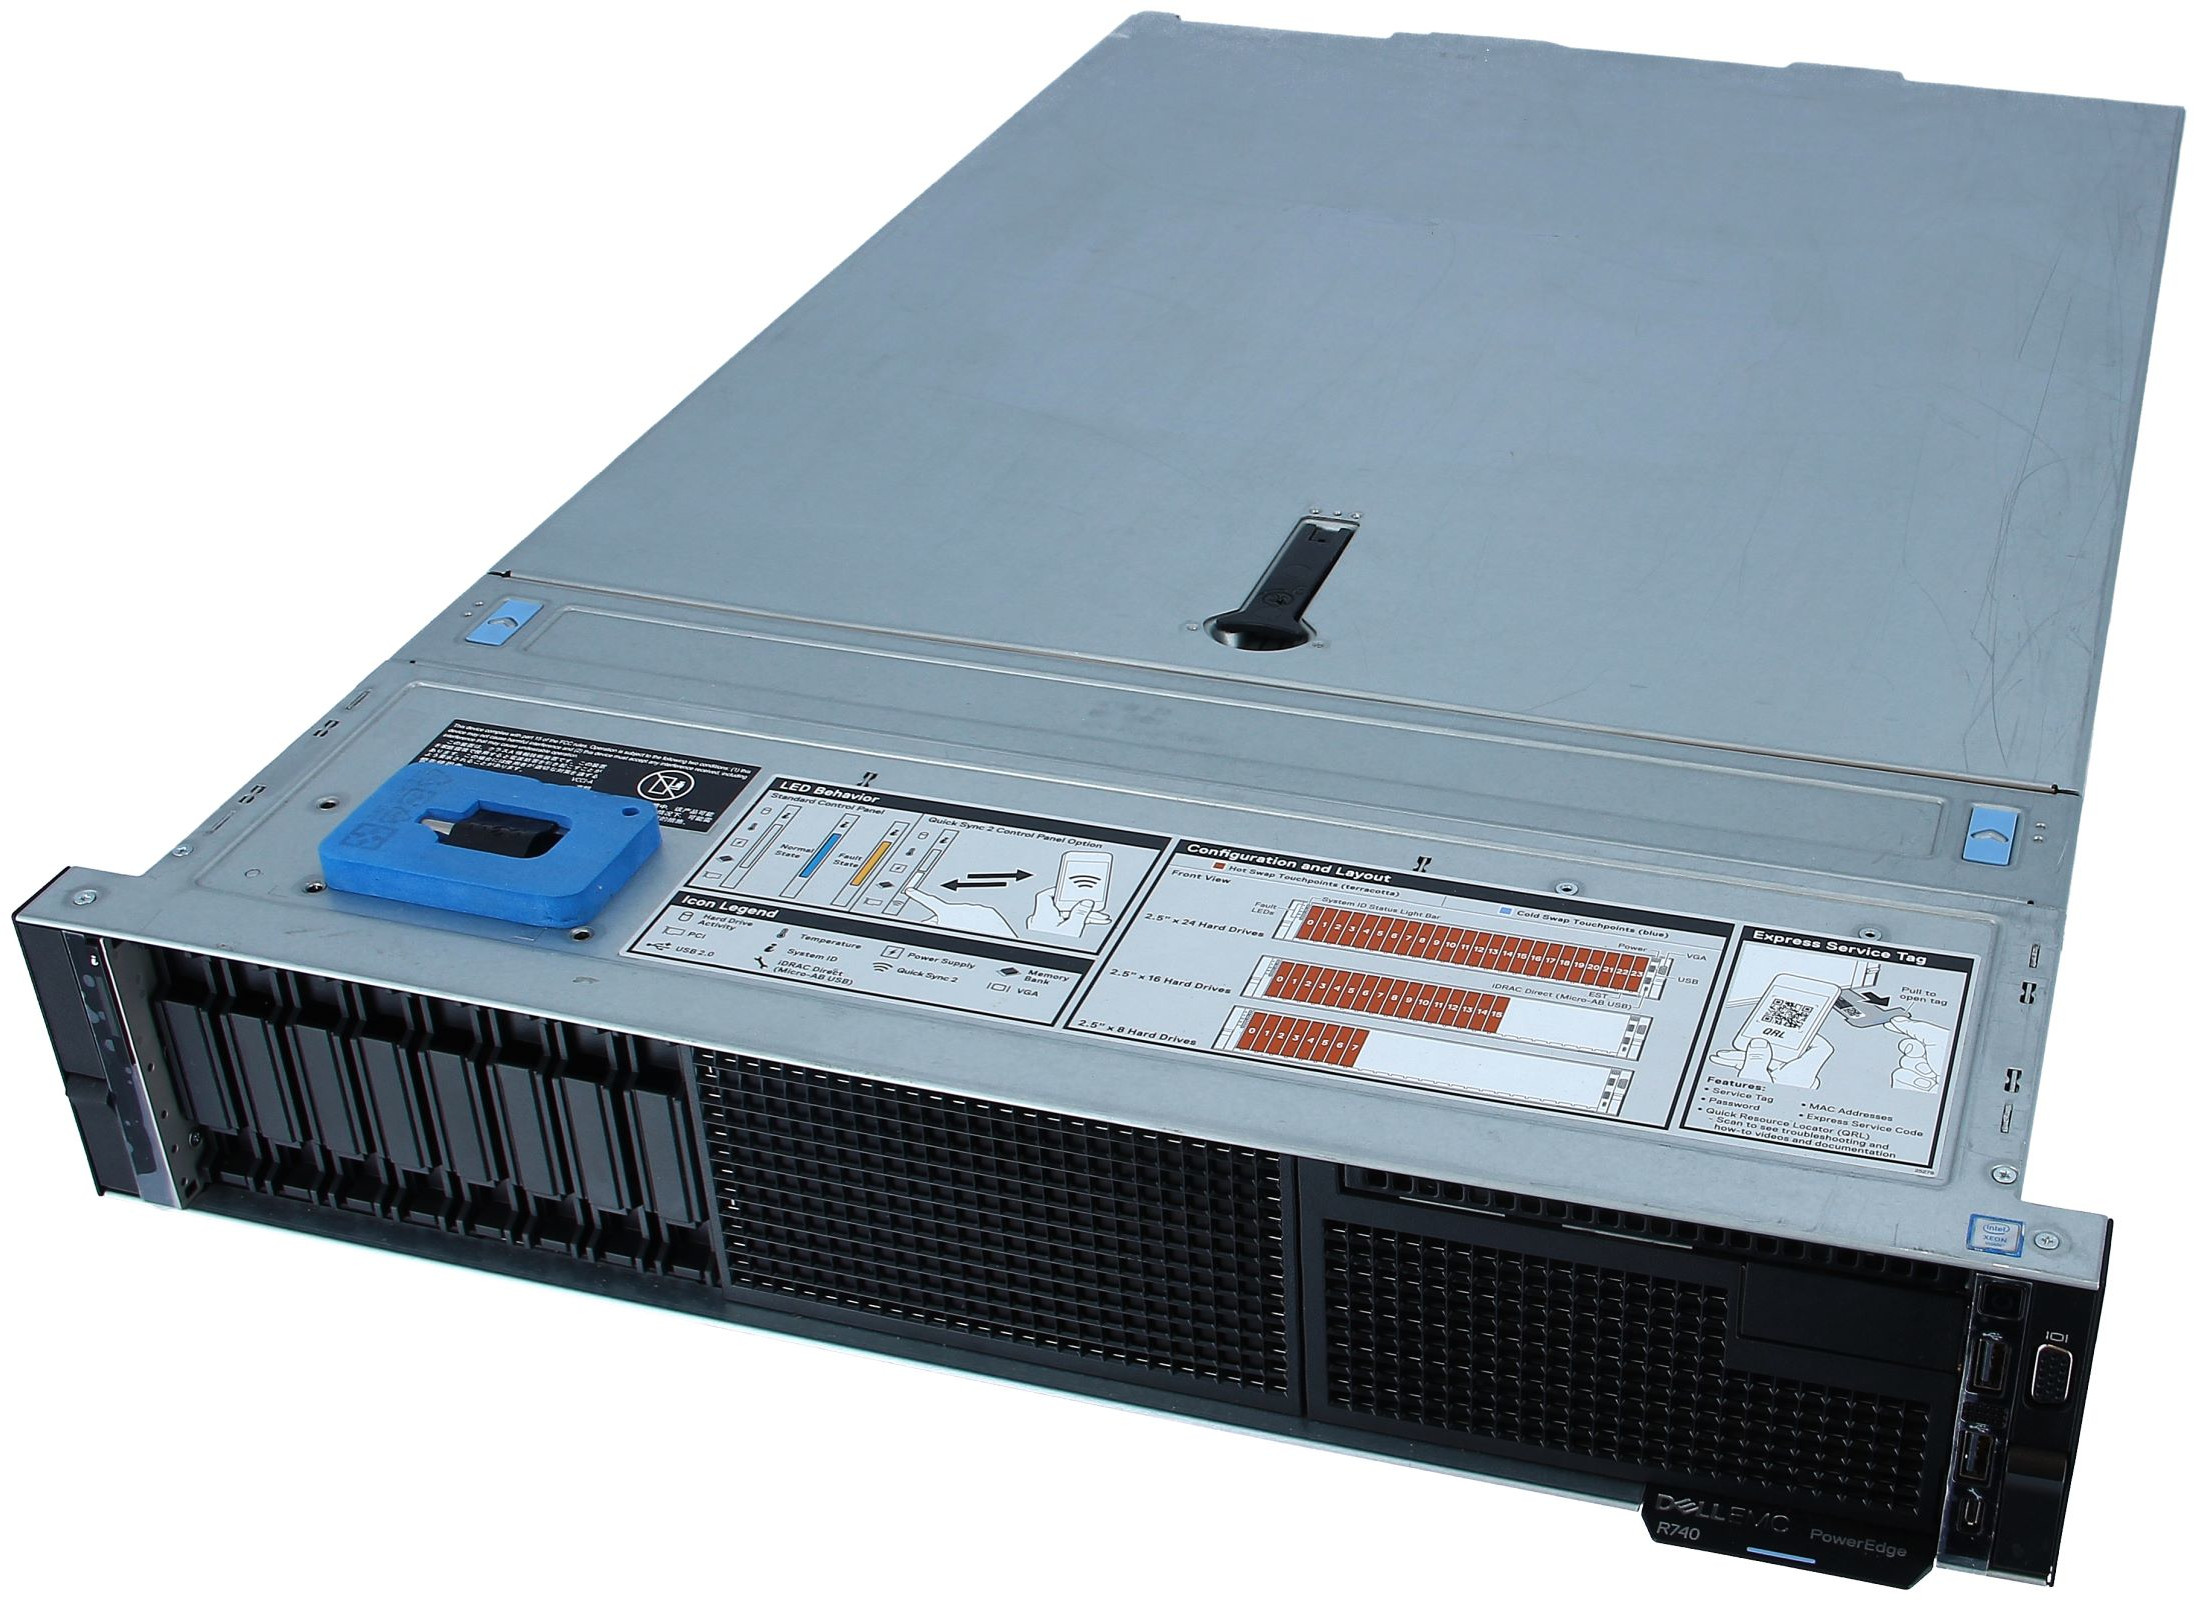
\includegraphics[width=3cm]{dell1}};
      \draw[<-, ultra thick] (Pi) -- (cable);
      \draw[->, ultra thick] (cable) -- (Pj);
    \end{scope}
  \end{tikzpicture}  
  
  \begin{block}{$P_i$ sends a message to \textbf{\alert{any other}} process $P_j$}
    \begin{itemize}
    \item Reasonable to assume \alert{$T = \alpha + n \times \beta$}, where
      \begin{itemize}
      \item $n =$ message size (bits)
      \item $\alpha =$ \alert{latency} (s)
      \item $\beta = 1 / $ \alert{bandwidth} (s / bit).
      \end{itemize}

      \medskip

    \item Assumption: \alert{full-duplex}
      \begin{itemize}
      \item Processes can send \& receive at the same time
      \end{itemize}

    \item $T$ \alert{independent} of $i, j$ (no weird topology)
    \item $T$ \alert{independent} from actions of other processes
      \begin{itemize}
      \item No congestion
      \end{itemize}
    \end{itemize}
  \end{block}
\end{frame}

\subsection{Network Topologies}

%%%%%%%%%%%%%%%%%%%%%%%%%%%%%%%%%%%%%%%%%%%%%%%%%%%%%%%%%%%%%%%%%

\begin{frame}
  \frametitle{Realistic?}
  \framesubtitle{Fat Tree (Infiniband / Omnipath)}

  \centering
  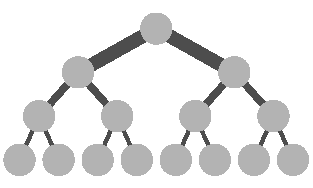
\includegraphics[width=10cm]{fat_tree.pdf}
\end{frame}

%%%%%%%%%%%%%%%%%%%%%%%%%%%%%%%%%%%%%%%%%%%%%%%%%%%%%%%%%%%%%%%

\begin{frame}
  \frametitle{Fat tree (2 levels)}
  
  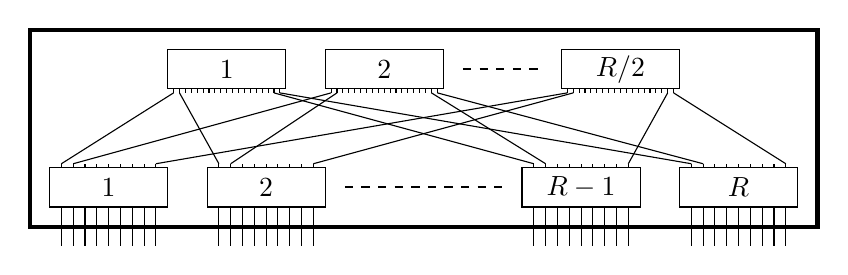
\begin{tikzpicture}[scale=0.5]
  \draw[ultra thick] (-0.5, -0.5) rectangle (19.5, 4.5);
  \draw[dashed, thick] (10.5, 3.5) -- (12.5, 3.5);
  \draw[dashed, thick] (7.5, 0.5) -- (11.5, 0.5);
  
  \foreach \j / \lab in {3/1, 7/2, 13/{$R/2$}} {
    \begin{scope}[xshift=\j*1cm]
      \draw (0, 3) rectangle node {\lab} +(3, 1);
      \foreach \i in {1, 2, ..., 19} {
        \draw (0.15*\i, 3) -- +(0, -0.1);
      }
    \end{scope}
  }

  \foreach \j / \lab in {0/1, 4/2, 12/{$R-1$}, 16/{$R$}} {
    \begin{scope}[xshift=\j*1cm]
      \draw (0, 0) rectangle node {\lab} +(3, 1);
      \foreach \i in {1, 2, ..., 9} {
        \draw (0.3*\i, 0) -- +(0, -1);
        \draw (0.3*\i, 1) -- +(0, 0.1);
      }
    \end{scope}
  }

  \draw (0 + 0.3*1, 1.1) -- (3 + 0.15*1, 2.9);
  \draw (0 + 0.3*2, 1.1) -- (7 + 0.15*1, 2.9);
  \draw (0 + 0.3*9, 1.1) -- (13 + 0.15*1, 2.9);

  \draw (4 + 0.3*1, 1.1) -- (3 + 0.15*2, 2.9);
  \draw (4 + 0.3*2, 1.1) -- (7 + 0.15*2, 2.9);
  \draw (4 + 0.3*9, 1.1) -- (13 + 0.15*2, 2.9);

  \draw (12 + 0.3*1, 1.1) -- (3 + 0.15*18, 2.9);
  \draw (12 + 0.3*2, 1.1) -- (7 + 0.15*18, 2.9);
  \draw (12 + 0.3*9, 1.1) -- (13 + 0.15*18, 2.9);

  \draw (16 + 0.3*1, 1.1) -- (3 + 0.15*19, 2.9);
  \draw (16 + 0.3*2, 1.1) -- (7 + 0.15*19, 2.9);
  \draw (16 + 0.3*9, 1.1) -- (13 + 0.15*19, 2.9);
\end{tikzpicture}

\bigskip

\begin{itemize}
\item \textbf{non-blocking} $R$-port ``basic'' switches
\item $(R^2 / 2)$-port switch using $1.5R$ basic switches
\item Infiniband : $R = 36 \leadsto $ 648 ports
\end{itemize}

\end{frame}

%%%%%%%%%%%%%%%%%%%%%%%%%%%%%%%%%%%%%%%%%%%%%%%%%%%%%%%%%%%%

\begin{frame}
  \frametitle{Infiniband 648-port ``Director'' switch }
  \begin{columns}
    \begin{column}{0.3\textwidth}
      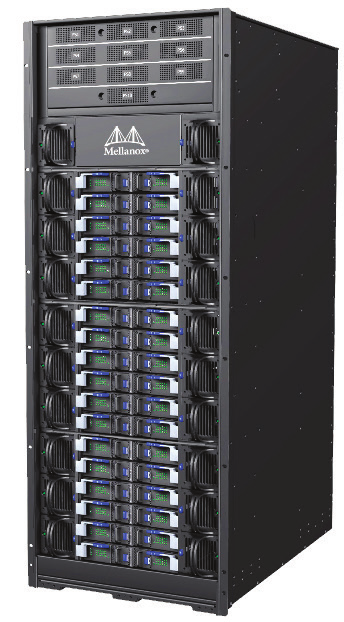
\includegraphics[height=0.75\textheight]{infiniband.png}

      \small image: (c) Mellanox
    \end{column}
    \begin{column}{0.6\textwidth}
      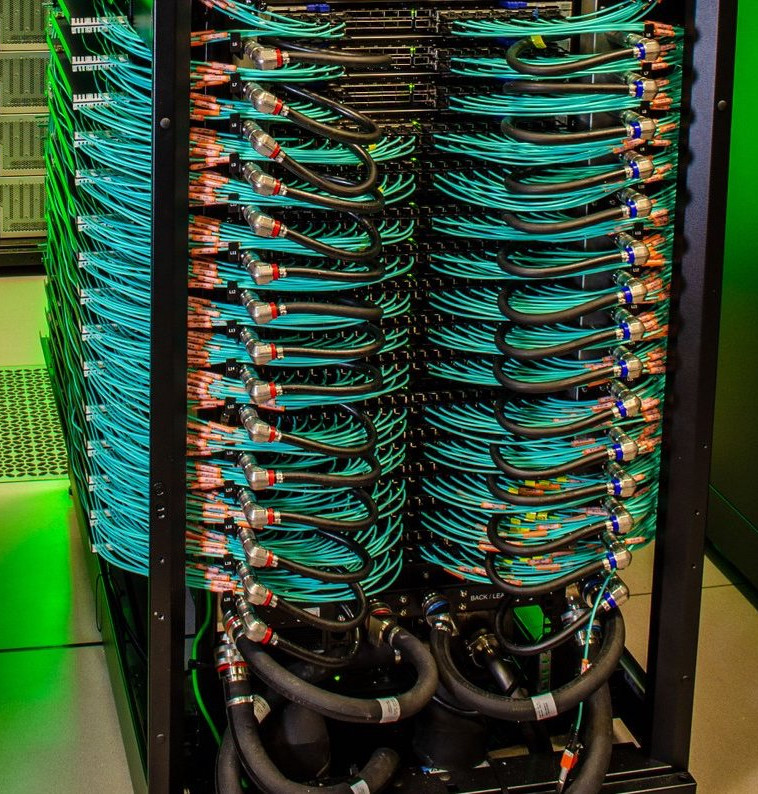
\includegraphics[height=0.75\textheight]{frontera_infiniband_director.jpg}

      \small image: (c) UTexas
    \end{column}
  \end{columns}
\end{frame}

%%%%%%%%%%%%%%%%%%%%%%%%%%%%%%%%%%%%%%%%%%%%%%%%%%%%%%%%%%%%%

\begin{frame}
  \frametitle{Fat tree (3 levels)}
  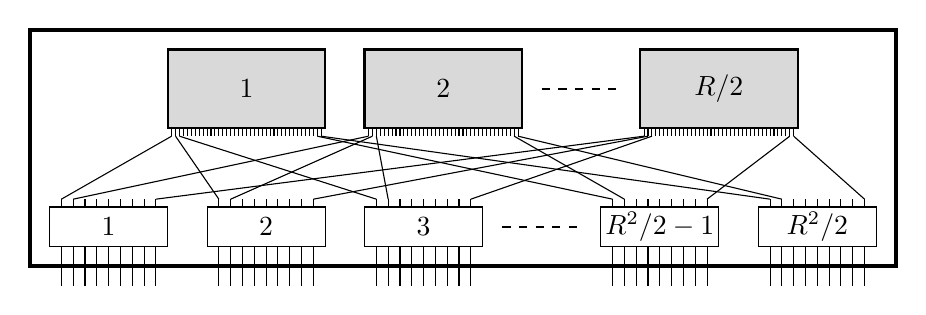
\begin{tikzpicture}[scale=0.5]
   \draw[ultra thick] (-0.5, -0.5) rectangle (21.5, 5.5);
   \draw[dashed, thick] (12.5, 4) -- (14.5, 4);
   \draw[dashed, thick] (11.5, 0.5) -- (13.5, 0.5);
  
  \foreach \j / \lab in {3/1, 8/2, 15/{$R/2$}} {
    \begin{scope}[xshift=\j*1cm]
      \draw[fill=gray!30, thick] (0, 3) rectangle node {\lab} +(4, 2);
      \foreach \i in {1, 2, ..., 39} {
        \draw (0.1*\i, 3) -- +(0, -0.2);
      }
    \end{scope}
  }

  \foreach \j / \lab in {0/1, 4/2, 8/3, 14/{$R^2/2-1$}, 18/{$R^2/2$}} {
    \begin{scope}[xshift=\j*1cm]
      \draw (0, 0) rectangle node {\lab} +(3, 1);
      \foreach \i in {1, 2, ..., 9} {
        \draw (0.3*\i, 0) -- +(0, -1);
        \draw (0.3*\i, 1) -- +(0, 0.2);
      }
    \end{scope}
  }

  \draw (0 + 0.3*1, 1.2) -- (3 + 0.1*1, 2.8);
  \draw (0 + 0.3*2, 1.2) -- (8 + 0.1*1, 2.8);
  \draw (0 + 0.3*9, 1.2) -- (15 + 0.1*1, 2.8);

  \draw (4 + 0.3*1, 1.2) -- (3 + 0.1*2, 2.8);
  \draw (4 + 0.3*2, 1.2) -- (8 + 0.1*2, 2.8);
  \draw (4 + 0.3*9, 1.2) -- (15 + 0.1*2, 2.8);

  \draw (8 + 0.3*1, 1.2) -- (3 + 0.1*3, 2.8);
  \draw (8 + 0.3*2, 1.2) -- (8 + 0.1*3, 2.8);
  \draw (8 + 0.3*9, 1.2) -- (15 + 0.1*3, 2.8);

  
  \draw (14 + 0.3*1, 1.2) -- (3 + 0.1*38, 2.8);
  \draw (14 + 0.3*2, 1.2) -- (8 + 0.1*38, 2.8);
  \draw (14 + 0.3*9, 1.2) -- (15 + 0.1*38, 2.8);

  \draw (18 + 0.3*1, 1.2) -- (3 + 0.1*39, 2.8);
  \draw (18 + 0.3*2, 1.2) -- (8 + 0.1*39, 2.8);
  \draw (18 + 0.3*9, 1.2) -- (15 + 0.1*39, 2.8);
\end{tikzpicture}

\bigskip


\begin{itemize}
\item Same technique, recursively
\item $(R^3 / 4)$-ports with $1.25 R^2$ basic $R$-port switches
\item Infiniband : $R = 36 \leadsto 11\ 644$ ports
\item Used in \texttt{Summit} with $9\ 216$ CPUs
  \begin{itemize}
  \item 1 rack = 18 nodes = 36 CPUs = 36 NICs
  \item Two 36-port switches per rack
  \item 256 racks
  \item 15 ``director'' (level-2) switches
  \end{itemize}
\end{itemize}
\end{frame}

%%%%%%%%%%%%%%%%%%%%%%%%%%%%%%%%%%%%%%%%%%%%%%%%%%%%%%%%%%%%%%

\begin{frame}
  \frametitle{Fat tree --- High Cabling Costs}
  \framesubtitle{It ends up looking like this}

  \centering
  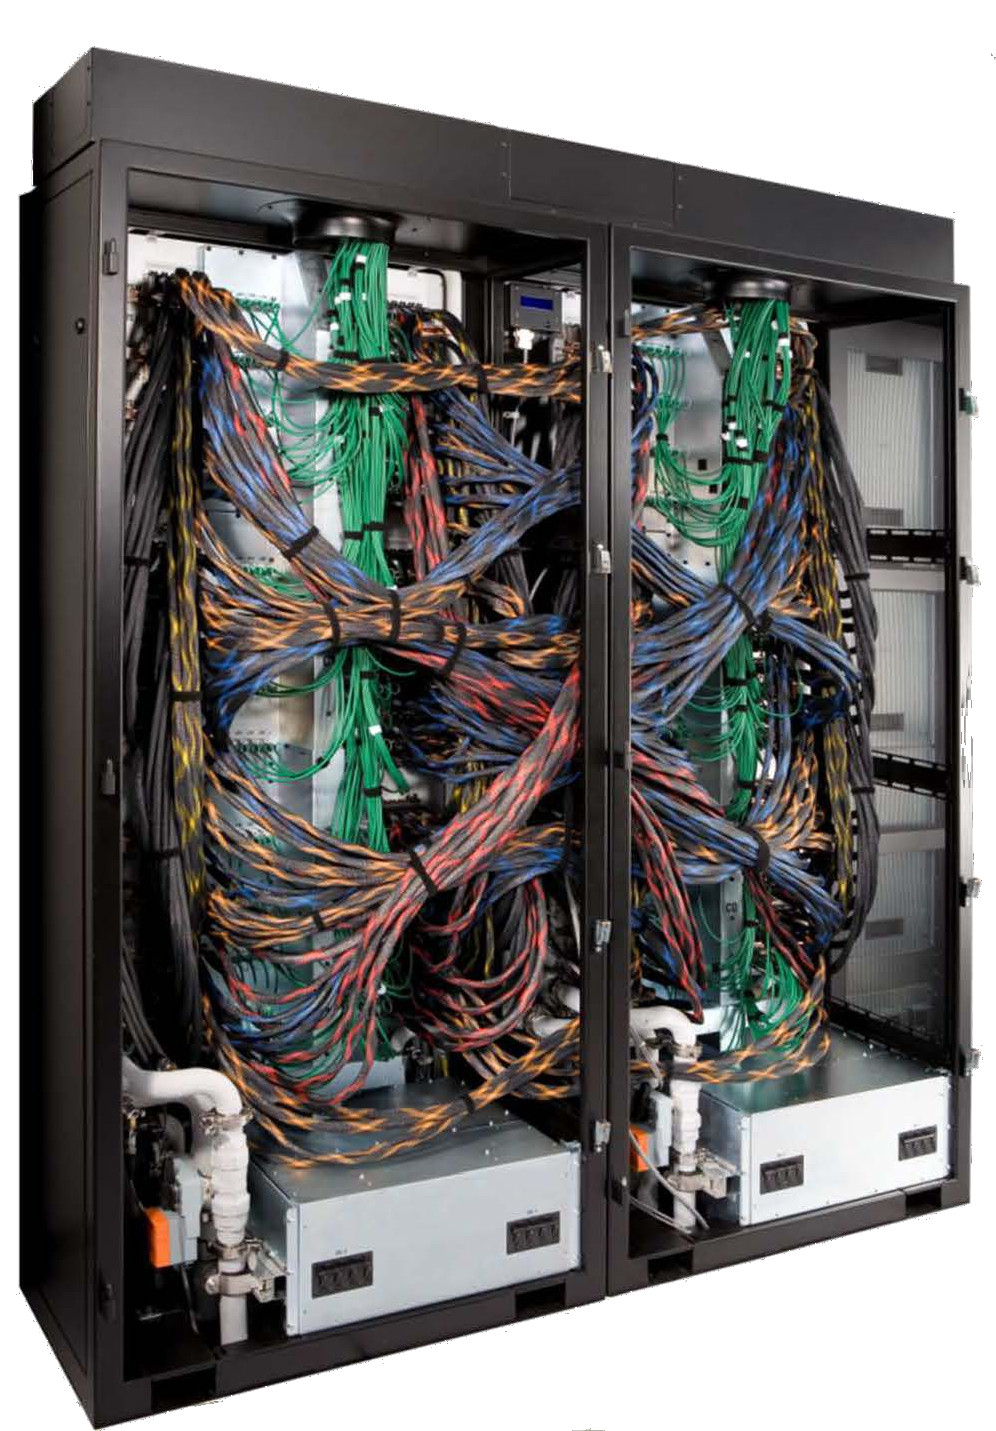
\includegraphics[height=8cm]{wiring}
\end{frame}

%%%%%%%%%%%%%%%%%%%%%%%%%%%%%%%%%%%%%%%%%%%%%%%%%%%%%%%%%%%%%%%

\begin{frame}[label=fat]
  \frametitle{Fat tree --- High Cabling Costs}

  \begin{center}
    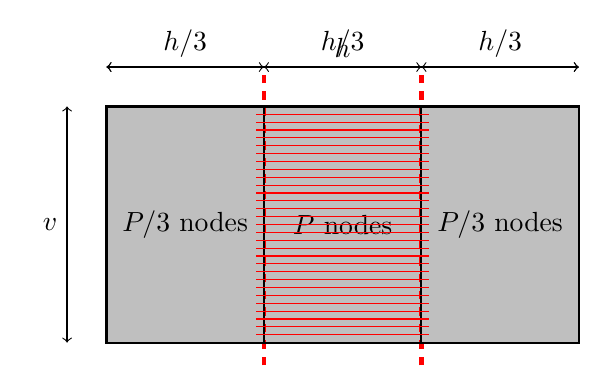
\begin{tikzpicture}
      \path[use as bounding box] (-1, 0) rectangle (6, 4);
      \draw[<->] (-0.5, 0) -- node[left] {$v$} +(0, 3);
      \draw<1-2>[<->] (0, 3.5) -- node[above] {$h$} +(6, 0);
      \draw<3->[<->] (0, 3.5) -- node[above] {$h/3$} +(2, 0);
      \draw<3->[<->] (2, 3.5) -- node[above] {$h/3$} +(2, 0);
      \draw<3->[<->] (4, 3.5) -- node[above] {$h/3$} +(2, 0);
      
      \draw<1-2>[thick, fill=lightgray] (0, 0) rectangle node {$P$ nodes} +(6, 3);

      \draw<2>[ultra thick, red, dashed] (2, -0.5) -- +(0, 4);
      \draw<2>[ultra thick, red, dashed] (4, -0.5) -- +(0, 4);   
      
      \draw<3->[thick, fill=lightgray] (0, 0) rectangle node {$P/3$ nodes} +(2, 3);
      \draw<3->[thick, fill=lightgray] (4, 0) rectangle node {$P/3$ nodes} +(2, 3);
      \draw<3->[thick] (2, 0) -- +(2, 0);
      \draw<3->[thick] (2, 3) -- +(2, 0);
      
      \foreach \i in {0.1, 0.2, ..., 2.9} {
        \draw<4->[red] (1.9, \i) -- (4.1, \i);
      } 
    \end{tikzpicture}
  \end{center}
  \begin{itemize}
  \item<2-> Split machine in 3
  \item<3-> All nodes on the left send messages to nodes on the right
  \item<4-> Assumption = no congestion
    \begin{itemize}
    \item[$\leadsto$] Need $P/3$ parallel network links across the middle
    \item[$\leadsto$] Length $\geq h/3$
    \end{itemize}
  \item<5->[$\Longrightarrow$] cable length $\geq hP/9 = \alert{\bigOmega{P^{1.5}}}$
  \item<5-> Fat tree a viable options with ``small'' \#nodes ($\leq$ 10k) 
  \end{itemize}
\end{frame}

%%%%%%%%%%%%%%%%%%%%%%%%%%%%%%%%%%%%%%%%%%%%%%%%%%%%%%%%%%%%%%%

\begin{frame}
  \frametitle{Cost-Saving Alternatives}
  \framesubtitle{3D Torus (IBM BlueGene/P, Cray XT3, ...)}

  \begin{center}
    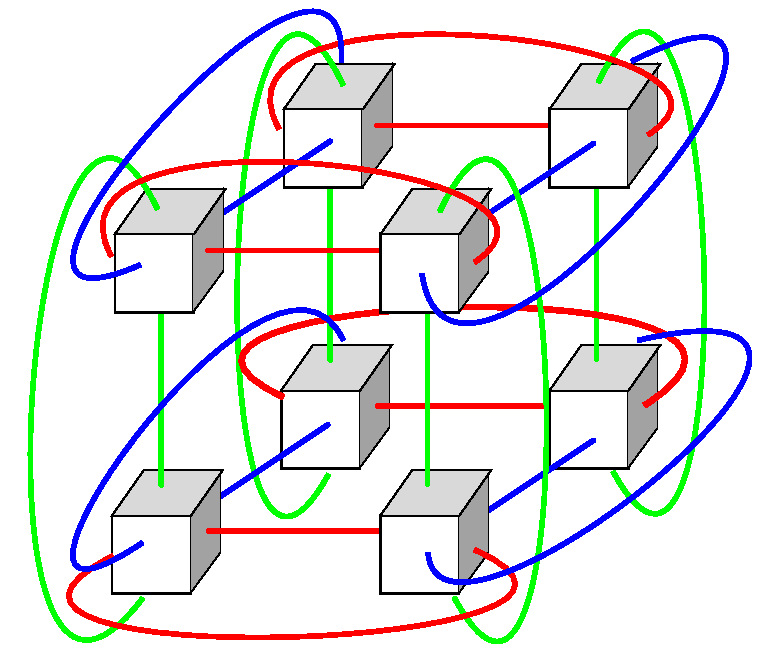
\includegraphics[height=6cm]{2x2x2torus.pdf}
  \end{center}

  \begin{itemize}
  \item Cable length \alert{proportional} to \#Nodes
  \item Used on very large machines
    \begin{itemize}
    \item E.g. $48 \times 72 \times 24 \approx 100$k Nodes
    \end{itemize}
  \end{itemize}
\end{frame}


\begin{frame}
  \frametitle{Cost-Saving Alternatives}
  \framesubtitle{5D Torus (IBM BlueGene/Q)}

  \centering
  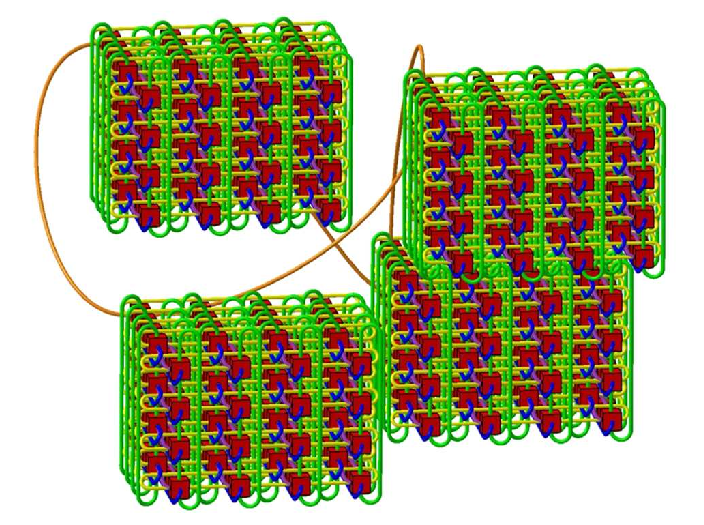
\includegraphics[height=8cm]{5D_torus.pdf}
\end{frame}

\begin{frame}
  \frametitle{Compromise}
  \framesubtitle{Dragonfly (Cray ``Aries'' Interconnect)}

  \centering
  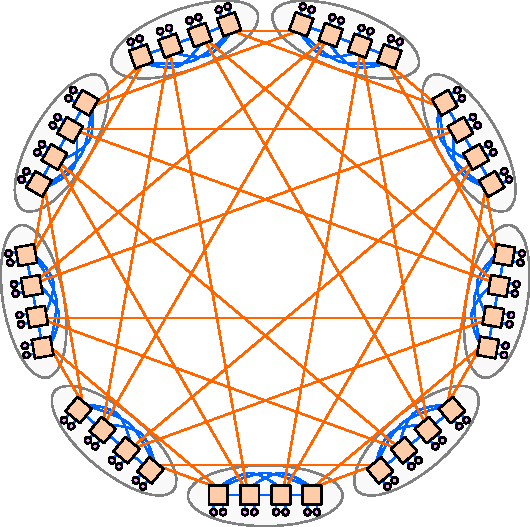
\includegraphics[height=8cm]{dragonfly.pdf}
\end{frame}

%%%%%%%%%%%%%%%%%%%%%%%%%%%%%%%%%%%%%%%%%%%%%%%%%%%%%%%%%%%%%%%%%%%%%%%%%%%%%%

\begin{frame}
  \frametitle{On Grid5000 ?}
  Except in special case, all nodes of a cluster connected to a switch

  MPI All-to-All:
  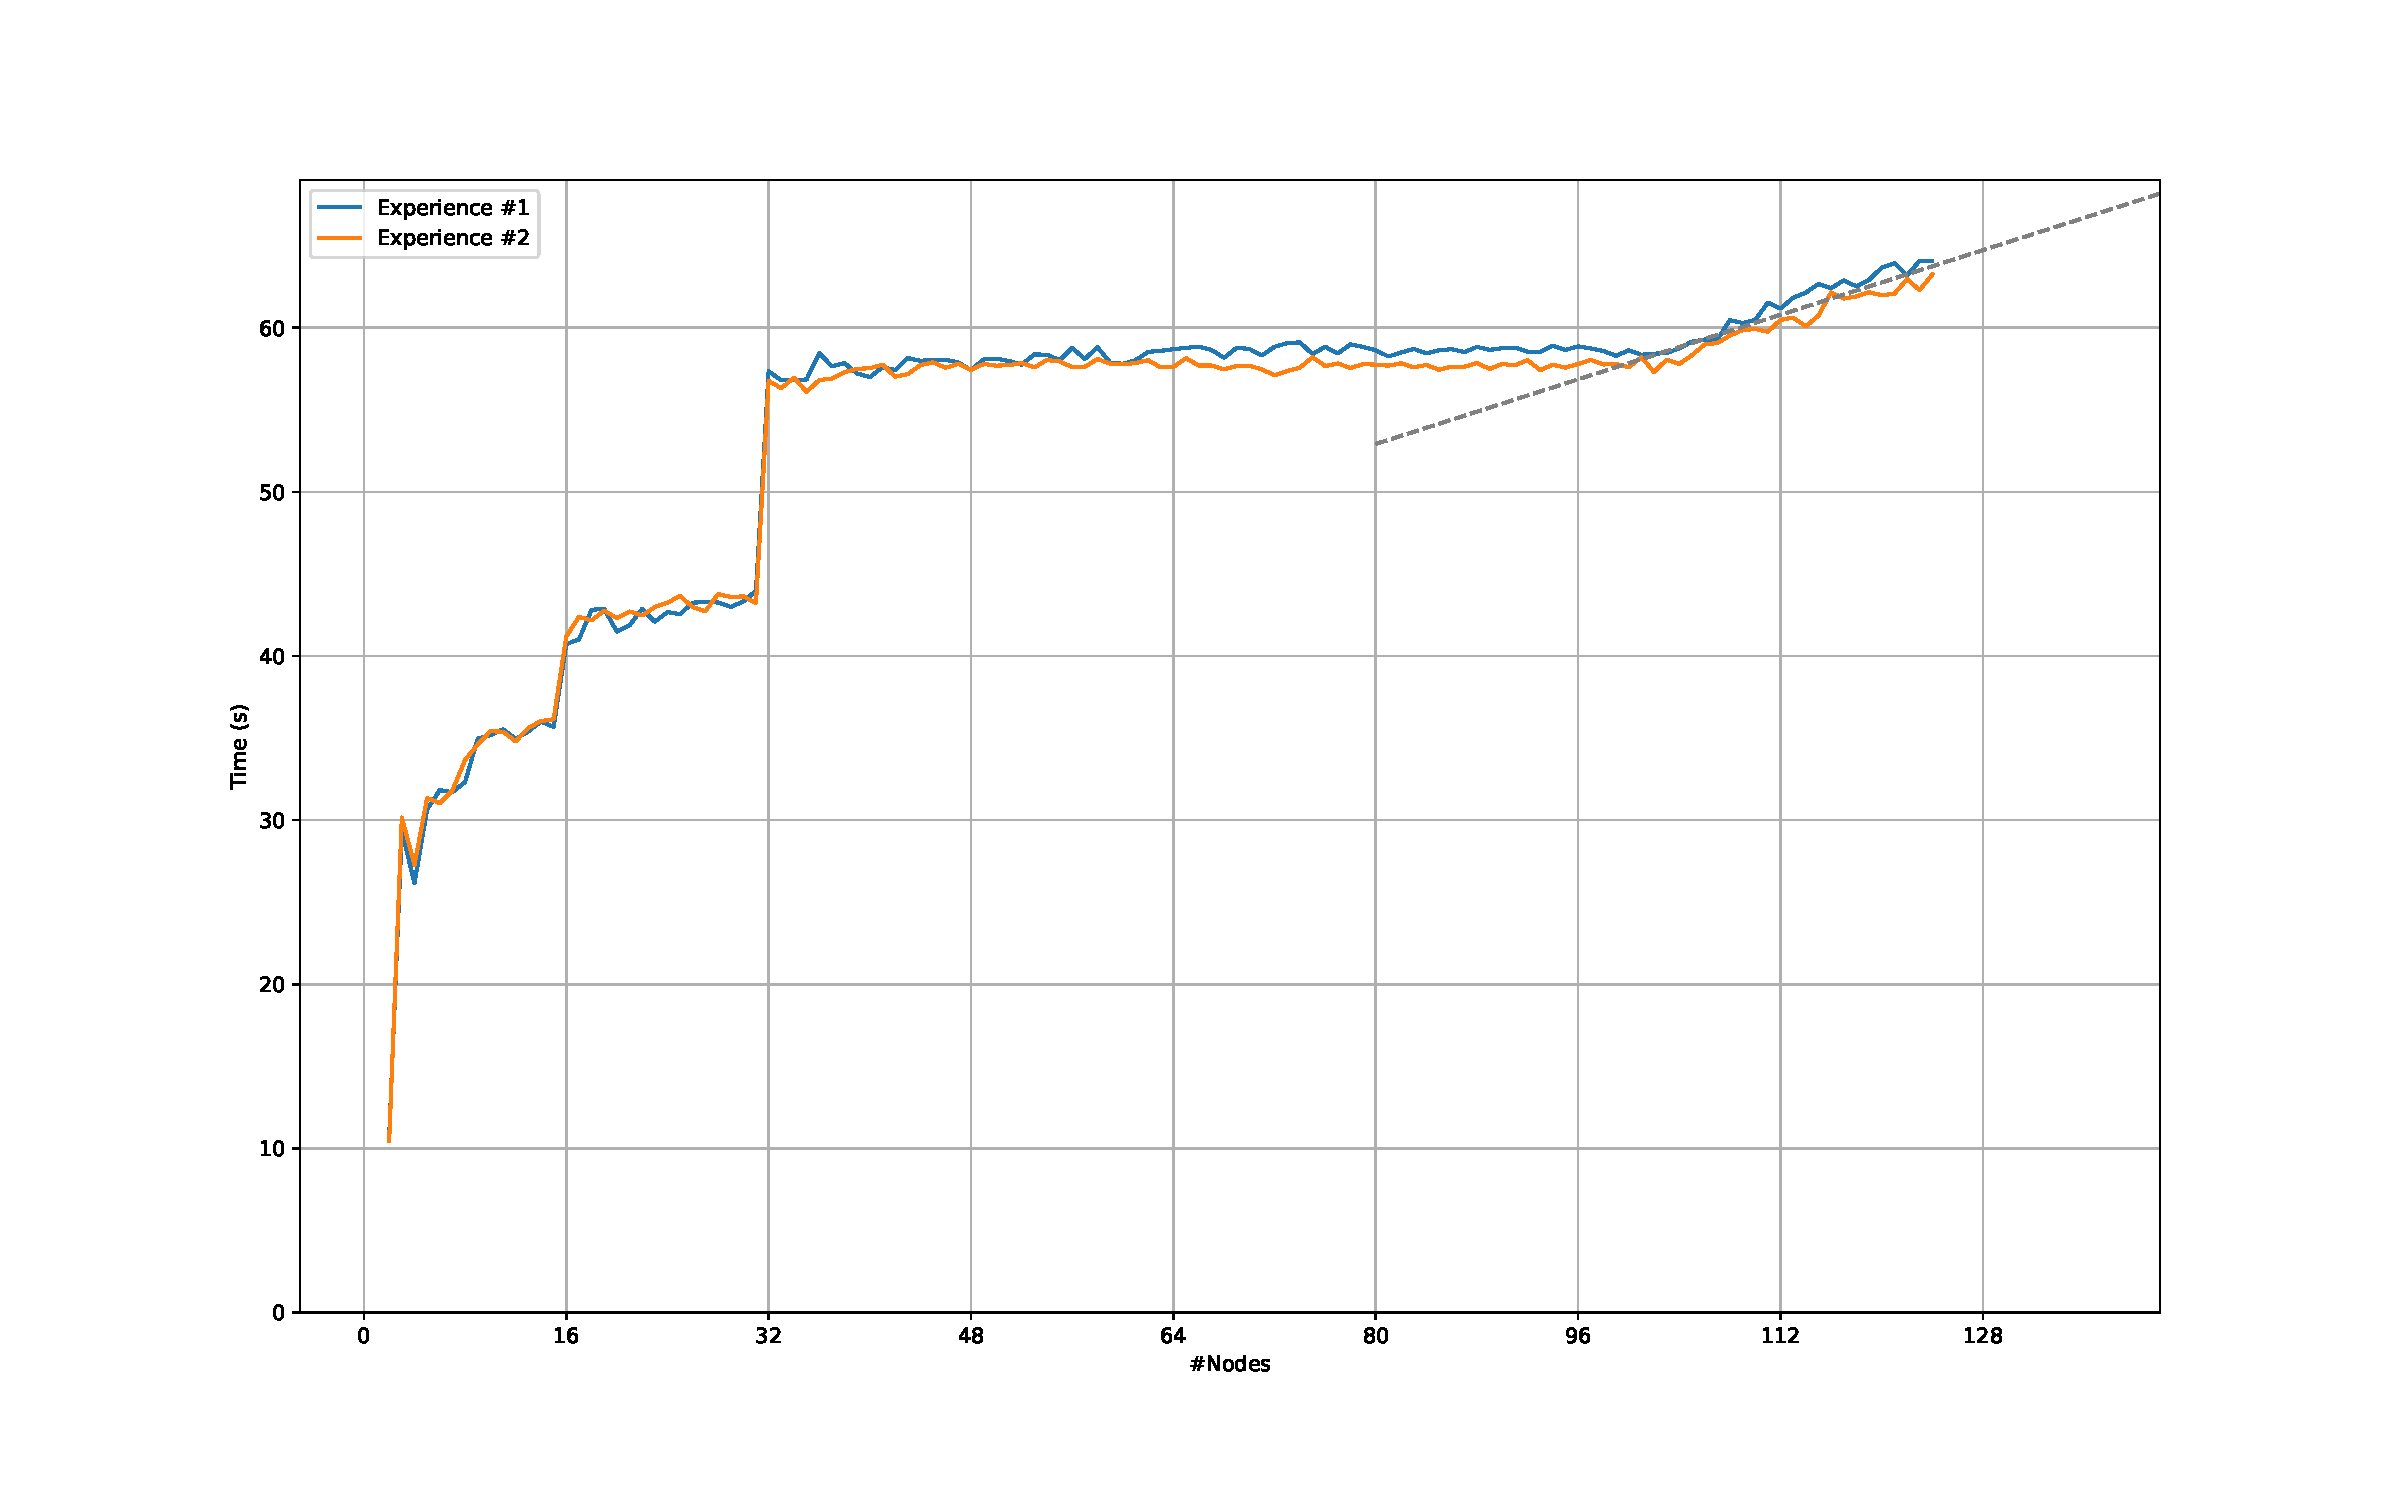
\includegraphics[width=\textwidth]{gros_sort.pdf}
\end{frame}

\begin{frame}
  \frametitle{On Grid5000 ?}

  Ring algorithm:
  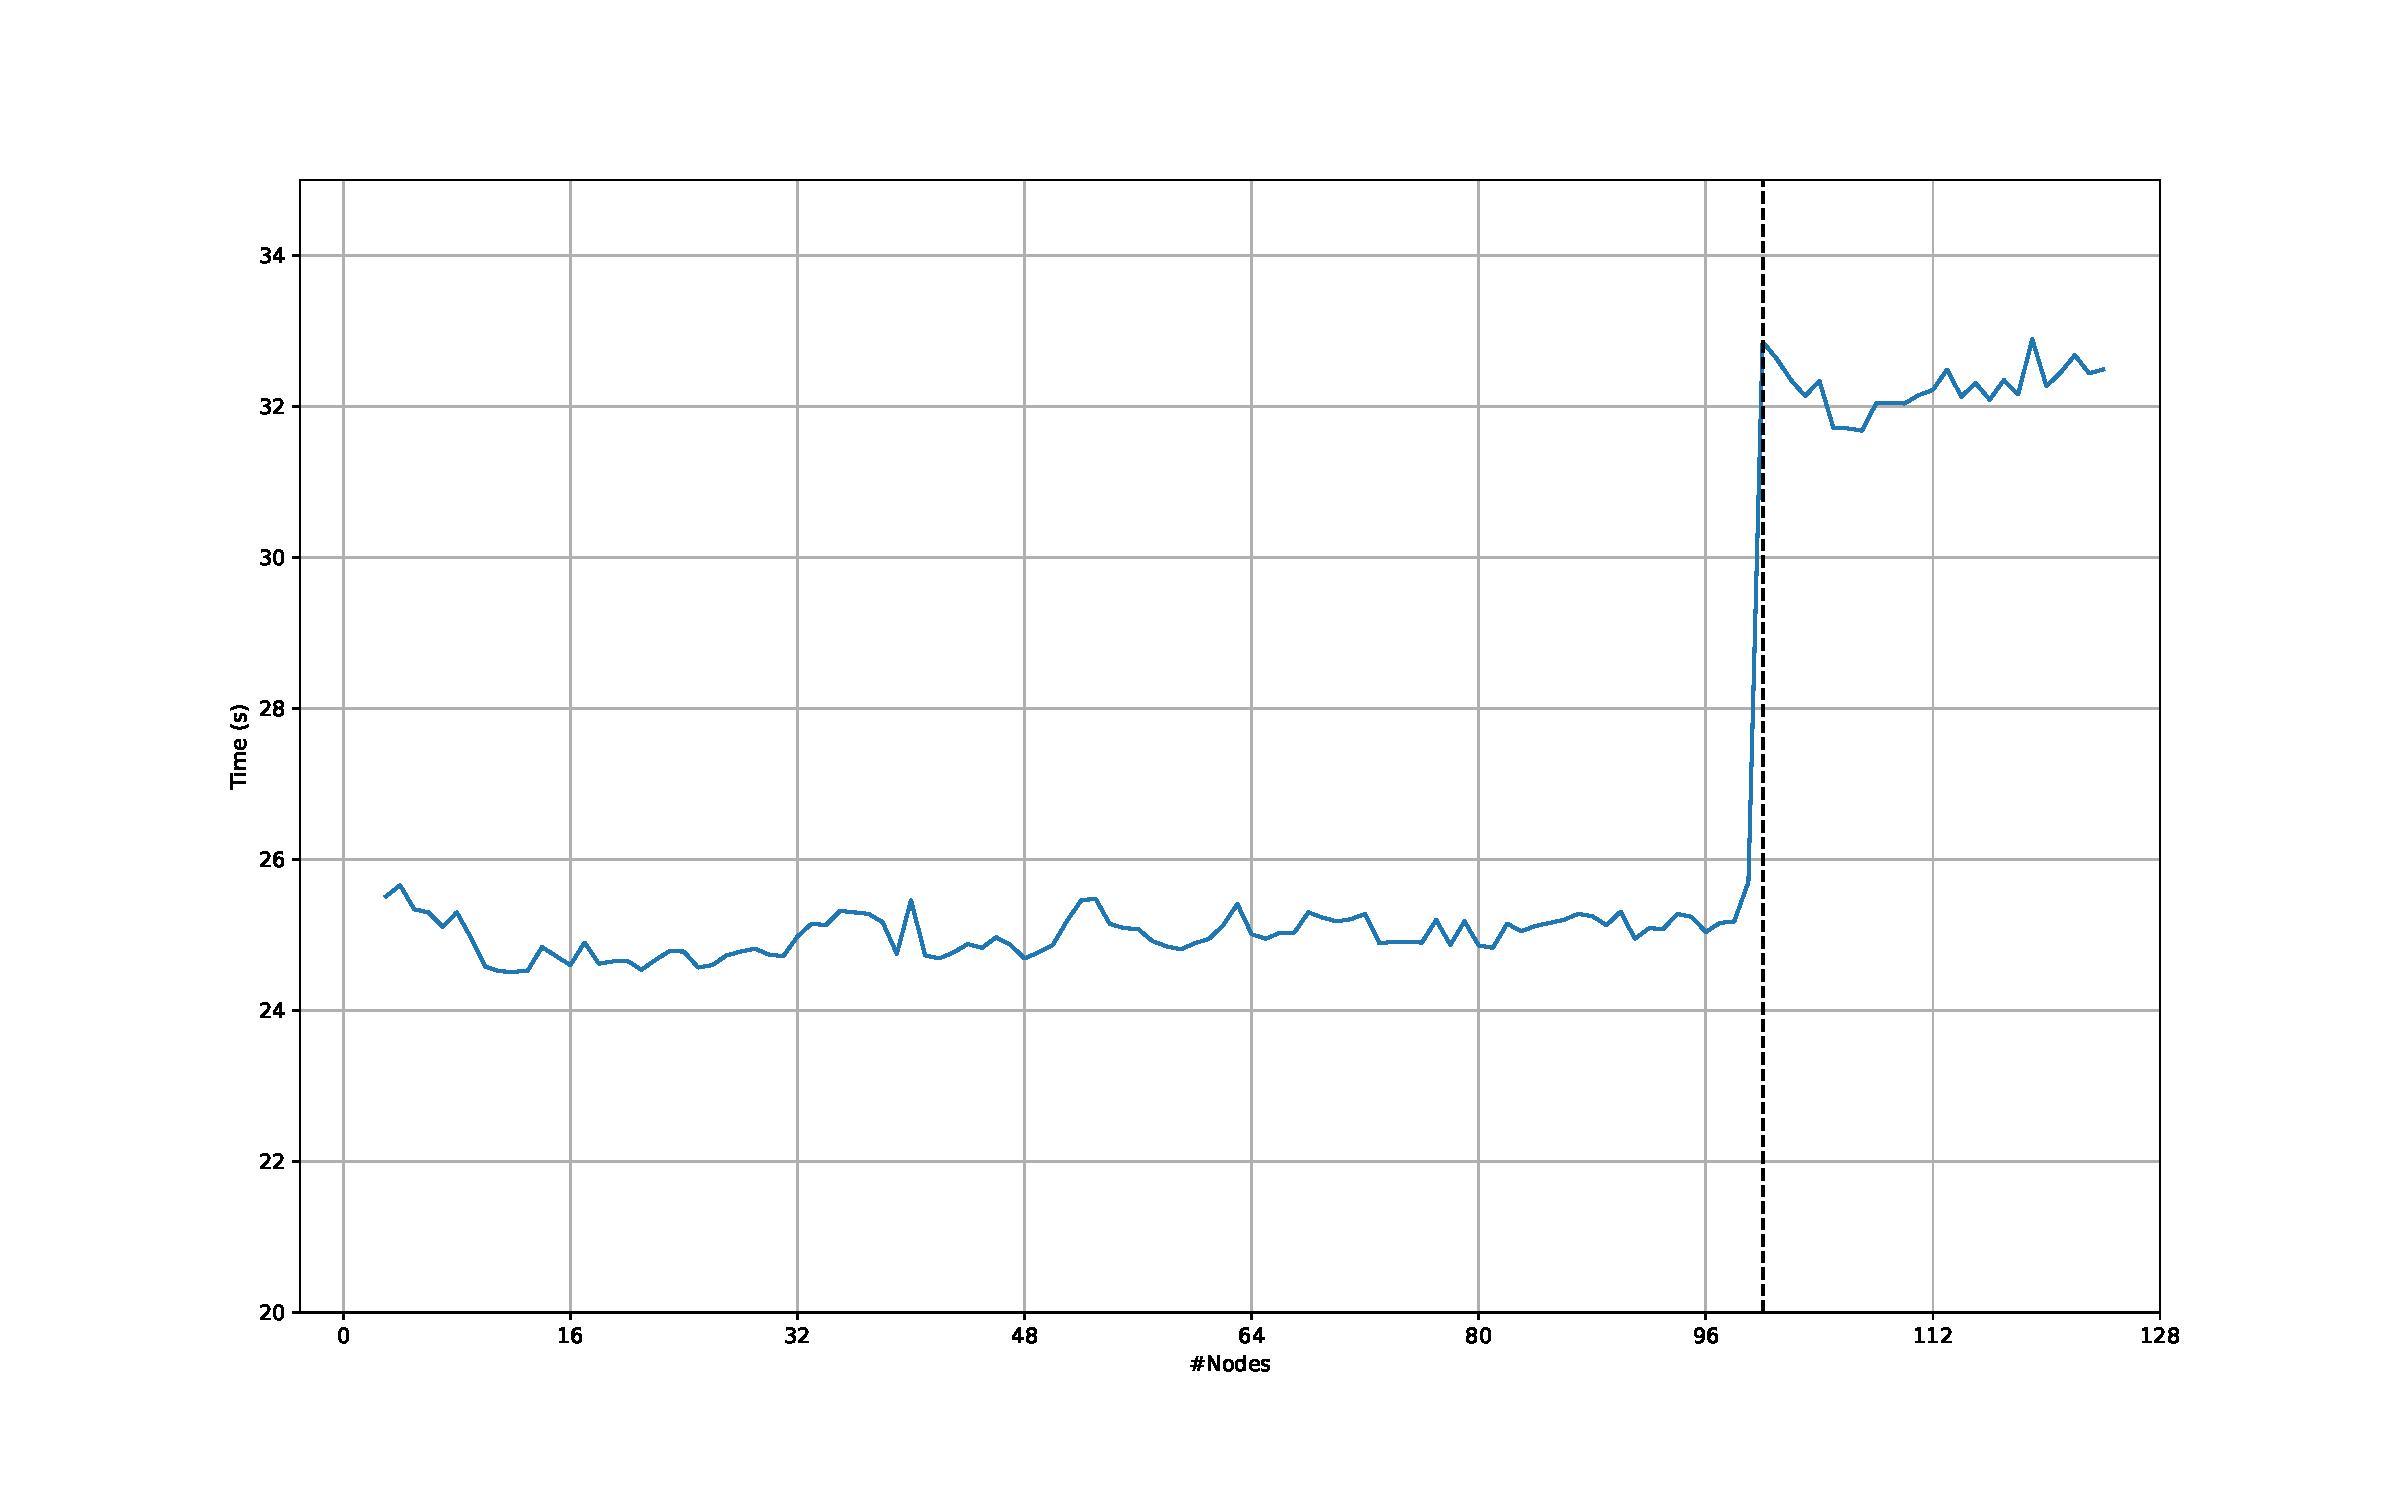
\includegraphics[width=\textwidth]{gros_cyclic.pdf}
\end{frame}

%%%%%%%%%%%%%%%%%%%%%%%%%%%%%%%%%%%%%%%%%%%%%%%%%%%%%%%%%%%%%%%%%%%%%%%%%%%%%%

\subsection{Scatter / Gather again}
\begin{frame}[label=red]
  \frametitle{Scatter/Gather Again: Binary Tree Algorithm}

  \begin{center}
    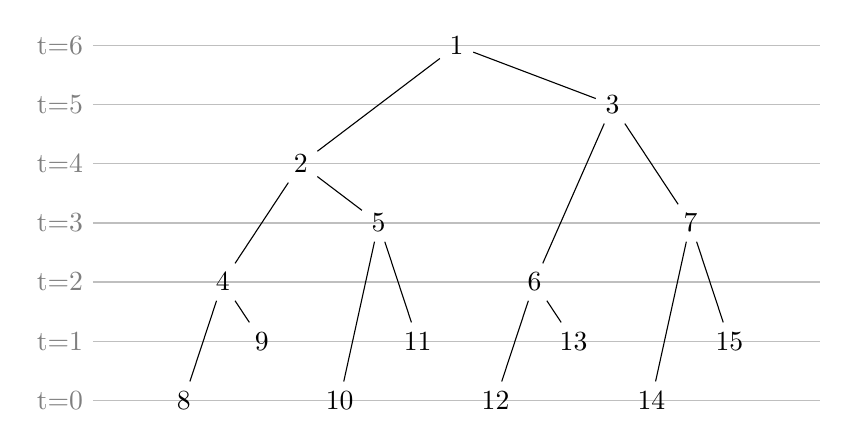
\begin{tikzpicture}[level distance=10mm, xscale=0.66, yscale=0.75]
  \foreach \i in {0,1,2,3,4,5,6} {
    \draw[semitransparent,gray] (-7, -6+\i) node[text=black,left] {t=\i} -- +(14, 0);
  }

  \node {1}
    child  { node at (0, -1) {2}
      child { node at (0,-1) {4}
        child {node at (0, -1) {8}}
        child {node  {9}}
      }
      child[missing]
      child {node  {5}
        child {node at (0, -2) {10}}
        child {node at (0, -1) {11}}
      }
    }
    child[missing]
    child[missing]
    child[missing]
     child { node {3}
      child {node at (0, -2) {6}
        child {node at (0, -1) {12} }
        child {node at (0, 0) {13} }
      }
      child[missing]
      child {node  at (0, -1) {7}
        child {node at (0, -2) {14}}
        child {node at (0, -1) {15} }
      }
    }
;
\end{tikzpicture}
\end{center}

\begin{itemize}
\item $2^{h+1} - 1$ nodes in total ; $2h$ successive messages
\item $2^{h-i}$ nodes of height $i$. Each transfers:
  \begin{itemize}
  \item Upwards $(2^{i+1}-1) n/p$ items
  \item Downwards $2\times (2^{i} - 1) n/p$ items 
  \end{itemize}

\item[$\Rightarrow$] $T \leq \alert{2} \lceil \log_2 P \rceil \alpha + \alert{2} (p-1)/p n\beta$
\end{itemize}
\end{frame}

%%%%%%%%%%%%%%

\begin{frame}
  \frametitle{Scatter/Gather Again: \textbf{Binomial} Tree Algorithm}
  
  \begin{center}
    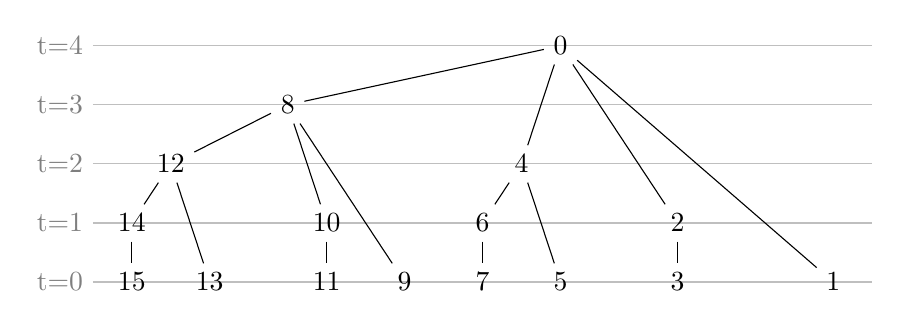
\begin{tikzpicture}[level distance=10mm, xscale=0.66, yscale=0.75]
  \foreach \i in {0,1,2,3,4} {
    \draw[semitransparent,gray] (-9, -4+\i) node[text=black,left] {t=\i} -- +(15, 0);
  }

  \node {0}
    child { node {8}
      child { node {12}
        child {node {14}
          child {node {15}}
        }
        child {node at (0, -1) {13}}
      }
      child[missing]
      child {node at (0,-1) {10}
        child {node {11}}
      }
      child {node at (0,-2) {9} }
    }
    child[missing]
    child[missing]
    child { node at (0, -1) {4}
      child {node {6}
        child {node {7} }
      }
      child {node at (0, -1) {5} }
    }
    child[missing]
    child { node at (0, -2) {2}
      child {node {3}}
    }
    child[missing]
    child { node at (0, -3) {1} }
;
\end{tikzpicture}
\end{center}

\begin{itemize}
\item $2^h$ nodes ; $h$ successive messages
\item Nodes of height $i$ transfer $2^i n/p$ items (synchronously) % send and receive the same quantity at the same time
\end{itemize}

\medskip
\begin{exampleblock}{\vspace*{-3ex}}
  \begin{align*}
    T &= \text{message of size 1 $+ \dots +$ message of size $n/2$} \\
      &= \alpha \lceil\log_2 p\rceil + \left(p - 1 \right)  \frac{n}{p} \beta \qquad \text{\alert{(optimal)}}
  \end{align*}
\end{exampleblock}
\end{frame}

%%%%%%%%%%%%%%%%%%%%%%%%%%%%%%%%%%%%%%%%%%%%%%%%%%%%

\begin{frame}
  \frametitle{Interlude: Binomial Tree}
  
  \begin{center}
    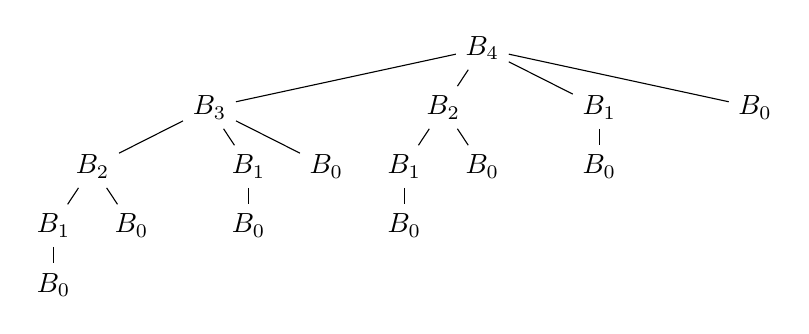
\begin{tikzpicture}[level distance=10mm, xscale=0.66, yscale=0.75]

  \node {$B_4$}
    child { node {$B_3$}
      child { node {$B_2$}
        child {node {$B_1$}
          child {node {$B_0$}}
        }
        child {node  {$B_0$}}
      }
      child[missing]
      child {node  {$B_1$}
        child {node {$B_0$}}
      }
      child {node  {$B_0$} }
    }
    child[missing]
    child[missing]
    child { node  {$B_2$}
      child {node {$B_1$}
        child {node {$B_0$} }
      }
      child {node  {$B_0$} }
    }
    child[missing]
    child { node  {$B_1$}
      child {node {$B_0$}}
    }
    child[missing]
    child { node {$B_0$} }
;
\end{tikzpicture}
\end{center}

\begin{itemize}
\item $B_i$ = root + $B_0 + B_1 + \dots B_{i-1}$
\item $B_i$ = $B_{i-1}$ + $B_{i-1}$
\item $\binom{h}{i}$ nodes at height $i$
\end{itemize}
\end{frame}


%%%%%%%%%%%%%%%%%%%%%%%%%%%%%%%%%%%%%%%%%%%%%%%%%%%

\subsection{Allgather}

\begin{frame}[label=alg]
\frametitle{AllGather again: Recursive Doubling Algorithm}

  \begin{center}
    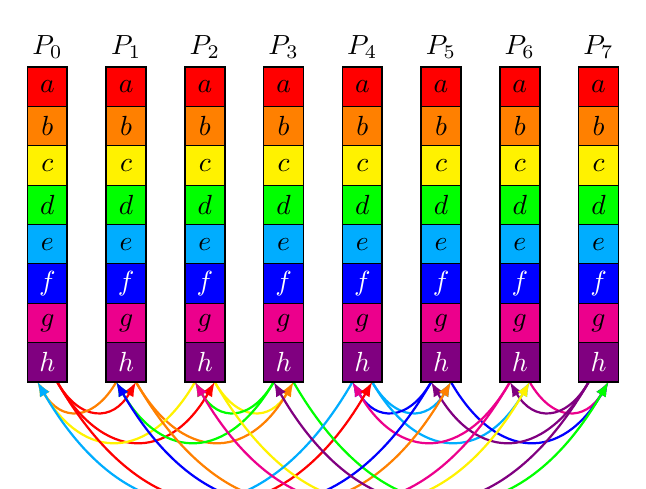
\begin{tikzpicture}[scale=0.5, >=latex]
      \useasboundingbox (0, -2) rectangle (15, 9);

      \foreach \i in {0,1,...,7} {
        \draw[thick] (2*\i, 0) rectangle +(1, 8);
        \foreach \j in {1,...,7} {
          \draw[thick] (2*\i, \j) -- +(1, 0);
        }
        \node at (2*\i + 0.5, 8.5) (P\i) {$P_\i$};
        \node[coordinate] at (2*\i + 0.25, 0) (l\i) {};
        \node[coordinate] at (2*\i + 0.75, 0) (r\i) {};
      }

      \filldraw[fill=red]     ( 0, 7) rectangle node {$a$}  +(1,1);
      \filldraw[fill=orange]  ( 2, 6) rectangle node {$b$} +(1,1);
      \filldraw[fill=yellow]  ( 4, 5) rectangle node {$c$} +(1,1);
      \filldraw[fill=green]   ( 6, 4) rectangle node {$d$} +(1,1);
      \filldraw[fill=cyan]    ( 8, 3) rectangle node {$e$} +(1,1);
      \filldraw[fill=blue]    (10, 2) rectangle node[white] {$f$} +(1,1);
      \filldraw[fill=magenta] (12, 1) rectangle node {$g$} +(1,1);
      \filldraw[fill=violet]  (14, 0) rectangle node[white] {$h$} +(1,1);

      \draw<2>[thick, red]    (r0) edge[->, bend right=60, looseness=1.5] (r1);
      \draw<2>[thick, orange] (l1) edge[->, bend left=60, looseness=1.5] (l0);
      \draw<2>[thick, yellow] (r2) edge[->, bend right=60, looseness=1.5] (r3);
      \draw<2>[thick, green]  (l3) edge[->, bend left=60, looseness=1.5] (l2);
      \draw<2>[thick, cyan]   (r4) edge[->, bend right=60, looseness=1.5] (r5);
      \draw<2>[thick, blue]   (l5) edge[->, bend left=60, looseness=1.5] (l4);
      \draw<2>[thick, magenta](r6) edge[->, bend right=60, looseness=1.5] (r7);
      \draw<2>[thick, violet] (l7) edge[->, bend left=60, looseness=1.5] (l6);

      \filldraw<3->[fill=red]     ( 2, 7) rectangle node {$a$}  +(1,1);
      \filldraw<3->[fill=orange]  ( 0, 6) rectangle node {$b$} +(1,1);
      \filldraw<3->[fill=yellow]  ( 6, 5) rectangle node {$c$} +(1,1);
      \filldraw<3->[fill=green]   ( 4, 4) rectangle node {$d$} +(1,1);
      \filldraw<3->[fill=cyan]    (10, 3) rectangle node {$e$} +(1,1);
      \filldraw<3->[fill=blue]    ( 8, 2) rectangle node[white] {$f$} +(1,1);
      \filldraw<3->[fill=magenta] (14, 1) rectangle node {$g$} +(1,1);
      \filldraw<3->[fill=violet]  (12, 0) rectangle node[white] {$h$} +(1,1);

      \draw<4>[thick, red]    (r0) edge[->, bend right=60, looseness=1.5] (r2);
      \draw<4>[thick, orange] (r1) edge[->, bend right=60, looseness=1.5] (r3);
      \draw<4>[thick, yellow] (l2) edge[->, bend left=60, looseness=1.5] (l0);
      \draw<4>[thick, green]  (l3) edge[->, bend left=60, looseness=1.5] (l1);
      \draw<4>[thick, cyan]   (r4) edge[->, bend right=60, looseness=1.5] (r6);
      \draw<4>[thick, blue]   (r5) edge[->, bend right=60, looseness=1.5]  (r7);
      \draw<4>[thick, magenta](l6) edge[->, bend left=60, looseness=1.5] (l4);
      \draw<4>[thick, violet] (l7) edge[->, bend left=60, looseness=1.5]  (l5);

      \filldraw<5->[fill=red]     ( 4, 7) rectangle node {$a$}  +(1,1);
      \filldraw<5->[fill=red]     ( 6, 7) rectangle node {$a$}  +(1,1);
      \filldraw<5->[fill=orange]  ( 4, 6) rectangle node {$b$} +(1,1);
      \filldraw<5->[fill=orange]  ( 6, 6) rectangle node {$b$} +(1,1);
      \filldraw<5->[fill=yellow]  ( 0, 5) rectangle node {$c$} +(1,1);
      \filldraw<5->[fill=yellow]  ( 2, 5) rectangle node {$c$} +(1,1);
      \filldraw<5->[fill=green]   ( 0, 4) rectangle node {$d$} +(1,1);
      \filldraw<5->[fill=green]   ( 2, 4) rectangle node {$d$} +(1,1);
      \filldraw<5->[fill=cyan]    (12, 3) rectangle node {$e$} +(1,1);
      \filldraw<5->[fill=cyan]    (14, 3) rectangle node {$e$} +(1,1);
      \filldraw<5->[fill=blue]    (12, 2) rectangle node[white] {$f$} +(1,1);
      \filldraw<5->[fill=blue]    (14, 2) rectangle node[white] {$f$} +(1,1);
      \filldraw<5->[fill=magenta] ( 8, 1) rectangle node {$g$} +(1,1);
      \filldraw<5->[fill=magenta] (10, 1) rectangle node {$g$} +(1,1);
      \filldraw<5->[fill=violet]  ( 8, 0) rectangle node[white] {$h$} +(1,1);
      \filldraw<5->[fill=violet]  (10, 0) rectangle node[white] {$h$} +(1,1);

      \draw<6>[thick, red]    (r0) edge[->, bend right=60, looseness=1.5] (r4);
      \draw<6>[thick, orange] (r1) edge[->, bend right=60, looseness=1.5] (r5);
      \draw<6>[thick, yellow] (r2) edge[->, bend right=60, looseness=1.5] (r6);
      \draw<6>[thick, green]  (r3) edge[->, bend right=60, looseness=1.5] (r7);
      \draw<6>[thick, cyan]   (l4) edge[->, bend left=60, looseness=1.5] (l0);
      \draw<6>[thick, blue]   (l5) edge[->, bend left=60, looseness=1.5] (l1);
      \draw<6>[thick, magenta](l6) edge[->, bend left=60, looseness=1.5]  (l2);
      \draw<6>[thick, violet] (l7) edge[->, bend left=60, looseness=1.5]  (l3);

      \foreach \i in {0, 2, ..., 14} {
        \filldraw<7->[fill=red]     (\i, 7) rectangle node {$a$}  +(1,1);
        \filldraw<7->[fill=orange]  (\i, 6) rectangle node {$b$} +(1,1);
        \filldraw<7->[fill=yellow]  (\i, 5) rectangle node {$c$} +(1,1);
        \filldraw<7->[fill=green]   (\i, 4) rectangle node {$d$} +(1,1);
        \filldraw<7->[fill=cyan]    (\i, 3) rectangle node {$e$} +(1,1);
        \filldraw<7->[fill=blue]    (\i, 2) rectangle node[white] {$f$} +(1,1);
        \filldraw<7->[fill=magenta] (\i, 1) rectangle node {$g$} +(1,1);
        \filldraw<7->[fill=violet]  (\i, 0) rectangle node[white] {$h$} +(1,1);
      }
      
    \end{tikzpicture}
  \end{center}
  
\bigskip

\begin{align*}
  T &= \text{msg of size $n/p$}  + \dots + \text{msg of size $n/4$} + \text{msg of size $n/2$} \\
    &= \alpha \log_2 p + (p-1) \frac{n}{p} \beta \qquad \text{\alert{(optimal)}}
\end{align*}
\end{frame}

%%%%%%%%%%%%%%%%%%%%%%%%%%%%%%%%%%%%%%%%%%%%%%%%%%%%

\subsection{Broacvast}

\begin{frame}
\frametitle{Algorithms for Broadcast / Reduce}

\begin{block}{Binomial Tree}
  \begin{itemize}
  \item $T = \lceil \log_2 p \rceil (\alpha + n \beta)$
  \item ``Bandwidth'' term sub-optimal
  \item (bad for large messages)
  \end{itemize}
\end{block}

\bigskip

\begin{block}{Van de Geijn}
  \begin{itemize}
  \item Broadcast = AllGather $\circ$ Scatter
    \begin{itemize}
    \item Recursive doubling / Binomial tree
    \end{itemize}
  \item $T = \alert{2}  (\log_2 p) \alpha +  \alert{2} \left(1 - \frac{1}{p}\right) n \beta$
  \item[$\rightarrow$] $2\times$ lower bound
  \end{itemize}
\end{block}
\end{frame}

\end{document}

%%%%%%%%%%%%%%%%%%%%%%%%%%%%%%%%%%%%%

\begin{frame}[fragile=singleslide]
  \frametitle{What About the MPI ``All-to-All'' Operation?!?}

  \begin{alertblock}{Exercise for next week}
    Design and analyse algorithms for \mintinline{C}{MPI_Alltoall} on
    \begin{itemize}
    \item 1D Torus
    \item 2D Torus
    \item Fat tree
    \end{itemize}
  \end{alertblock}
\end{frame}

%%%%%%%%%%%%%%%%%%%%%%%%%%%%%%%%%%%%%%%%%%%%%%%%%%%%%%%%%%%%%

\section{Prefix-Sum}

\begin{frame}[fragile]
\frametitle{Parallélisme de données}


\begin{block}{Exemple classique : \emph{prefix-sum} (``scan'') (en place)}
\begin{minted}{C}
for (int i = 1; i < n; i++)
    A[i] = A[i] + A[i - 1];
\end{minted}
\end{block}

\bigskip

\begin{itemize}
\item \textbf{Dépendance de données}
\item Chaque itération a besoin du résultat de la précédente...
\item Changer l'algorithme   
\end{itemize}
\end{frame}

%%%%%%%%%%%%%%%%%%%%%%%%%%%%%%%%%%%%%%%%%%%%%%%%%%%%%%%%%%%%%%%%

\begin{frame}[fragile]
\frametitle{\texttt{prefix-sum} : Cas de la mémoire partagée}


\begin{block}{Exemple classique : \emph{prefix-sum} (en place)}
\begin{minted}[fontsize=\small]{C}
double *B;

void prefix_sum(double * A, int n)
{
    if (n < 2)
        return;
    for (int i = 0; i < n / 2; i++)
        B[i] = A[2 * i] + A[2 * i + 1];
    prefix_sum(B, k);
    for (int i = 1; i < n; i += 2) {
          A[i] = B[i / 2];
          A[i + 1] = B[i / 2] + A[i + 1];
    }
}
\end{minted}
\end{block}


\end{frame}


%%%%%%%%%%%%%%%%%%%%%%%%%%%%%%%%%%%%%%%%%%%%%%%%%%%%%%%%%%%%%%%%%

\begin{frame}
\frametitle{Algorithme MIMD-DM pour \texttt{prefix-sum}}

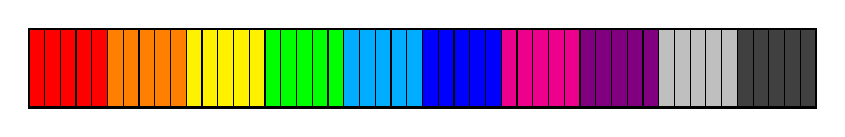
\begin{tikzpicture}
  \filldraw[fill=red]    (0, 0) rectangle  +(1,1);
  \filldraw[fill=orange] (1, 0) rectangle  +(1,1);
  \filldraw[fill=yellow] (2, 0) rectangle  +(1,1);
  \filldraw[fill=green]  (3, 0) rectangle  +(1,1);
  \filldraw[fill=cyan]   (4, 0) rectangle  +(1,1);
  \filldraw[fill=blue]   (5, 0) rectangle  +(1,1);
  \filldraw[fill=magenta] (6, 0) rectangle  +(1,1);
  \filldraw[fill=violet] (7, 0) rectangle +(1,1);
  \filldraw[fill=lightgray] (8, 0) rectangle +(1,1);
  \filldraw[fill=darkgray] (9, 0) rectangle +(1,1);
  
  \draw[thick] (0, 0) rectangle (10, 1);
  \foreach \i in {0.2, 0.4, ..., 9.8}
  \draw (\i, 0) -- +(0, 1);
\end{tikzpicture}

\bigskip

\begin{enumerate}
\item $P_i$ calcule la somme $S_i$ de \emph{ses} données. \hfill \alert{[local]}
\item Ils font (collectivement) $T \gets \texttt{prefix-sum}(S)$.
  \begin{itemize}
  \item \texttt{MPI\_Scan}
  \end{itemize}
\item[$\rightarrow$] $P_i$ obtient $T_i = $ somme des données des $P_j$ (pour $j<i$).
\item $P_i$ \texttt{prefix-sum} ses données en ajoutant $T_i$. \hfill \alert{[local]}
\end{enumerate}
\end{frame}

%%%%%%%%%%%%%%%%%%%%%%%%%%%%%%%%%%%%%%%%% 

\begin{frame}
  \frametitle{Rappel : \texttt{reduce} par la méthode de l'arbre binomial}
  
  \begin{center}
    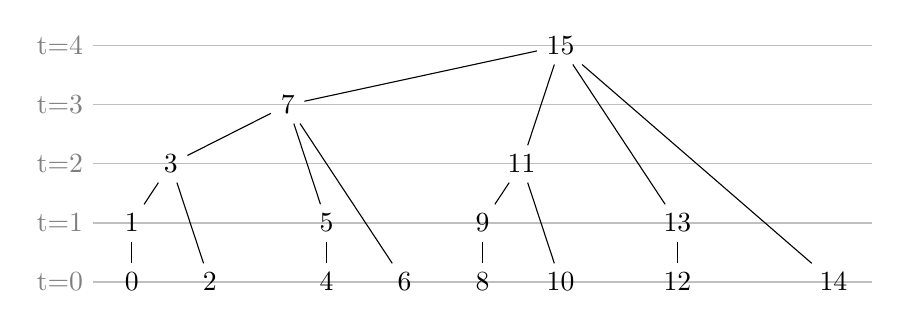
\begin{tikzpicture}[level distance=10mm, xscale=0.66, yscale=0.75]
  \foreach \i in {0,1,2,3,4} {
    \draw[semitransparent,gray] (-9, -4+\i) node[text=black,left] {t=\i} -- +(15, 0);
  }

  \node {15}
    child { node {7}
      child { node {3}
        child {node {1}
          child {node {0}}
        }
        child {node at (0, -1) {2}}
      }
      child[missing]
      child {node at (0,-1) {5}
        child {node {4}}
      }
      child {node at (0,-2) {6} }
    }
    child[missing]
    child[missing]
    child { node at (0, -1) {11}
      child {node {9}
        child {node {8} }
      }
      child {node at (0, -1) {10} }
    }
    child[missing]
    child { node at (0, -2) {13}
      child {node {12}}
    }
    child[missing]
    child { node at (0, -3) {14} }
;
\end{tikzpicture}
\end{center}


  \begin{center}
    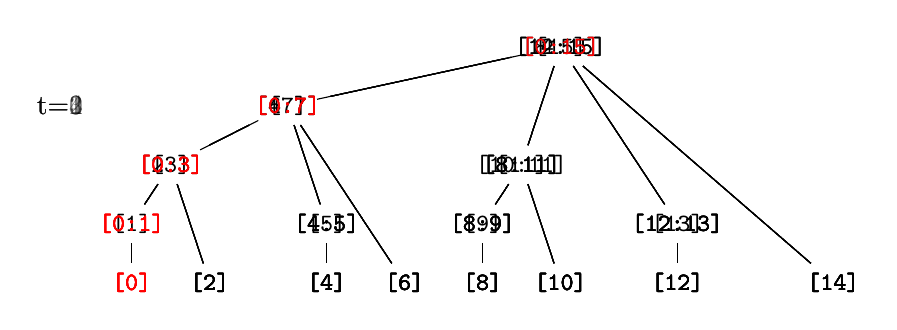
\begin{tikzpicture}[level distance=10mm, xscale=0.66, yscale=0.75]

      %%%
      \path<1> [semitransparent,gray] (-9, -1) node[text=black,left] {t=0};
      \path<2> [semitransparent,gray] (-9, -1) node[text=black,left] {t=1};
      \path<3> [semitransparent,gray] (-9, -1) node[text=black,left] {t=2};
      \path<4> [semitransparent,gray] (-9, -1) node[text=black,left] {t=3};
      \path<5> [semitransparent,gray] (-9, -1) node[text=black,left] {t=4};
      
      \begin{scope}[every node/.style={font=\small\ttfamily}]
          \node<1> {[15]}
    child { node {[7]}
      child { node {[3]}
        child {node {[1]}
          child {node[text=red] {[0]}}
        }
        child {node at (0, -1) {[2]}}
      }
      child[missing]
      child {node at (0,-1) {[5]}
        child {node {[4]}}
      }
      child {node at (0,-2) {[6]} }
    }
    child[missing]
    child[missing]
    child { node at (0, -1) {[11]}
      child {node {[9]}
        child {node {[8]} }
      }
      child {node at (0, -1) {[10]} }
    }
    child[missing]
    child { node at (0, -2) {[13]}
      child {node {[12]}}
    }
    child[missing]
    child { node at (0, -3) {[14]} }
    ;
    
    %%%%%%

    \node<2> {[14:15]}
    child { node {[6:7]}
      child { node {[2:3]}
        child {node[text=red] {[0:1]}
          child {node[text=red] {[0]}}
        }
        child {node at (0, -1) {[2]}}
      }
      child[missing]
      child {node at (0,-1) {[4:5]}
        child {node {[4]}}
      }
      child {node at (0,-2) {[6]} }
    }
    child[missing]
    child[missing]
    child { node at (0, -1) {[10:11]}
      child {node {[8:9]}
        child {node {[8]} }
      }
      child {node at (0, -1) {[10]} }
    }
    child[missing]
    child { node at (0, -2) {[12:13]}
      child {node {[12]}}
    }
    child[missing]
    child { node at (0, -3) {[14]} }
    ;

    %%%%%% 

    \node<3> {[12:15]}
    child { node {[4:7]}
      child { node [text=red] {[0:3]}
        child {node[text=red] {[0:1]}
          child {node[text=red] {[0]}}
        }
        child {node at (0, -1) {[2]}}
      }
      child[missing]
      child {node at (0,-1) {[4:5]}
        child {node {[4]}}
      }
      child {node at (0,-2) {[6]} }
    }
    child[missing]
    child[missing]
    child { node at (0, -1) {[8:11]}
      child {node {[8:9]}
        child {node {[8]} }
      }
      child {node at (0, -1) {[10]} }
    }
    child[missing]
    child { node at (0, -2) {[12:13]}
      child {node {[12]}}
    }
    child[missing]
    child { node at (0, -3) {[14]} }
    ;

    %%%%%% 

    \node<4> {[8:15]}
    child { node[text=red] {[0:7]}
      child { node [text=red] {[0:3]}
        child {node[text=red] {[0:1]}
          child {node[text=red] {[0]}}
        }
        child {node at (0, -1) {[2]}}
      }
      child[missing]
      child {node at (0,-1) {[4:5]}
        child {node {[4]}}
      }
      child {node at (0,-2) {[6]} }
    }
    child[missing]
    child[missing]
    child { node at (0, -1) {[8:11]}
      child {node {[8:9]}
        child {node {[8]} }
      }
      child {node at (0, -1) {[10]} }
    }
    child[missing]
    child { node at (0, -2) {[12:13]}
      child {node {[12]}}
    }
    child[missing]
    child { node at (0, -3) {[14]} }
    ;

    %%%%%% 

    \node<5>[text=red] {[0:15]}
    child { node[text=red] {[0:7]}
      child { node [text=red] {[0:3]}
        child {node[text=red] {[0:1]}
          child {node[text=red] {[0]}}
        }
        child {node at (0, -1) {[2]}}
      }
      child[missing]
      child {node at (0,-1) {[4:5]}
        child {node {[4]}}
      }
      child {node at (0,-2) {[6]} }
    }
    child[missing]
    child[missing]
    child { node at (0, -1) {[8:11]}
      child {node {[8:9]}
        child {node {[8]} }
      }
      child {node at (0, -1) {[10]} }
    }
    child[missing]
    child { node at (0, -2) {[12:13]}
      child {node {[12]}}
    }
    child[missing]
    child { node at (0, -3) {[14]} }
    ;

  \end{scope}
\end{tikzpicture}
\end{center}
\end{frame}

%%%%%%%%%%%%%%%%%%%%%%%%%%%%%%%%%%%%%%%%%%%

\begin{frame}
  \frametitle{\texttt{prefix-sum} en mémoire distribuée (arbre binomial)}

  \begin{exampleblock}{Phase 1 : \texttt{reduce}}
    Chaque noeud :
    \begin{enumerate}
    \item Récupère (et stocke) les valeurs de ses enfants.
    \item Calcule la somme, ajoute sa propre valeur, envoie à son père.
    \end{enumerate}
  \end{exampleblock}

  $\rightarrow \log_2$ messages successifs.
  
  \medskip

  \begin{alertblock}{Phase 2 : \texttt{prefix-sum}}
    Chaque noeud :
    \begin{enumerate}
    \item Reçoit une valeur de son père
      \begin{itemize}
      \item Somme des valeurs de ses frères \emph{gauches}.
        
      \end{itemize}
      
    \item Envoie à chacun de ses fils la somme des valeurs remontées par ses
      frères \emph{gauches}, plus la valeur reçue du père.
    \end{enumerate}
  \end{alertblock}

    $\rightarrow \log_2$ messages successifs.
\end{frame}

%%%%%%%%%%%%%%%%%%%%%%%%%%%%%%%%%%%

\begin{frame}<5->
  \frametitle{\texttt{prefix-sum} par la méthode de l'arbre binomial}
  

  \begin{center}
    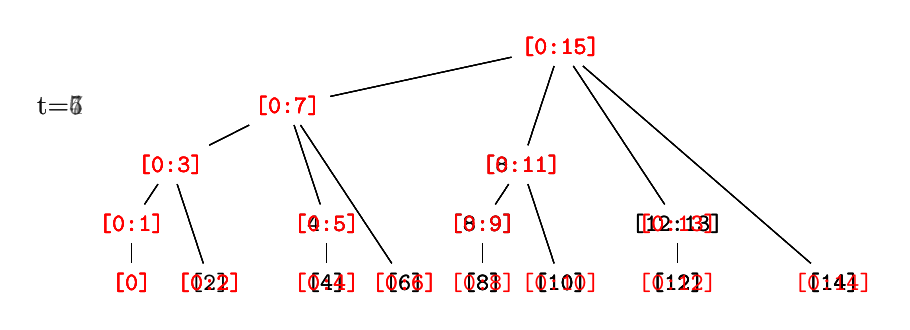
\begin{tikzpicture}[level distance=10mm, xscale=0.66, yscale=0.75]

      %%%
    \path<5> [semitransparent,gray] (-9, -1) node[text=black,left] {t=4};
    \path<6> [semitransparent,gray] (-9, -1) node[text=black,left] {t=5};
    \path<7> [semitransparent,gray] (-9, -1) node[text=black,left] {t=6};
    \path<8> [semitransparent,gray] (-9, -1) node[text=black,left] {t=7};
    
      \begin{scope}[every node/.style={font=\small\ttfamily}]

    \node<5>[text=red] {[0:15]}
    child { node[text=red] {[0:7]}
      child { node [text=red] {[0:3]}
        child {node[text=red] {[0:1]}
          child {node[text=red] {[0]}}
        }
        child {node at (0, -1) {[2]}}
      }
      child[missing]
      child {node at (0,-1) {[4:5]}
        child {node {[4]}}
      }
      child {node at (0,-2) {[6]} }
    }
    child[missing]
    child[missing]
    child { node at (0, -1) {[8:11]}
      child {node {[8:9]}
        child {node {[8]} }
      }
      child {node at (0, -1) {[10]} }
    }
    child[missing]
    child { node at (0, -2) {[12:13]}
      child {node {[12]}}
    }
    child[missing]
    child { node at (0, -3) {[14]} }
    ;


        \node<6>[text=red] {[0:15]}
    child { node[text=red] {[0:7]}
      child { node [text=red] {[0:3]}
        child {node[text=red] {[0:1]}
          child {node[text=red] {[0]}}
        }
        child {node[text=red] at (0, -1) {[0:2]}}
      }
      child[missing]
      child {node[text=red] at (0,-1) {[0:5]}
        child {node {[4]}}
      }
      child {node at (0,-2) {[6]} }
    }
    child[missing]
    child[missing]
    child { node[text=red] at (0, -1) {[0:11]}
      child {node {[8:9]}
        child {node {[8]} }
      }
      child {node at (0, -1) {[10]} }
    }
    child[missing]
    child { node at (0, -2) {[12:13]}
      child {node {[12]}}
    }
    child[missing]
    child { node at (0, -3) {[14]} }
    ;

    \node<7>[text=red] {[0:15]}
    child { node[text=red] {[0:7]}
      child { node [text=red] {[0:3]}
        child {node[text=red] {[0:1]}
          child {node[text=red] {[0]}}
        }
        child {node[text=red] at (0, -1) {[0:2]}}
      }
      child[missing]
      child {node[text=red] at (0,-1) {[0:5]}
        child {node[text=red] {[0:4]}}
      }
      child {node[text=red] at (0,-2) {[0:6]} }
    }
    child[missing]
    child[missing]
    child { node[text=red] at (0, -1) {[0:11]}
      child {node[text=red] {[0:9]}
        child {node {[8]} }
      }
      child {node at (0, -1) {[10]} }
    }
    child[missing]
    child { node[text=red] at (0, -2) {[0:13]}
      child {node {[12]}}
    }
    child[missing]
    child { node at (0, -3) {[14]} }
    ;

    \node<8>[text=red] {[0:15]}
    child { node[text=red] {[0:7]}
      child { node [text=red] {[0:3]}
        child {node[text=red] {[0:1]}
          child {node[text=red] {[0]}}
        }
        child {node[text=red] at (0, -1) {[0:2]}}
      }
      child[missing]
      child {node[text=red] at (0,-1) {[0:5]}
        child {node[text=red] {[0:4]}}
      }
      child {node[text=red] at (0,-2) {[0:6]} }
    }
    child[missing]
    child[missing]
    child { node[text=red] at (0, -1) {[0:11]}
      child {node[text=red] {[0:9]}
        child {node[text=red] {[0:8]} }
      }
      child {node[text=red] at (0, -1) {[0:10]} }
    }
    child[missing]
    child { node[text=red] at (0, -2) {[0:13]}
      child {node[text=red] {[0:12]}}
    }
    child[missing]
    child { node[text=red] at (0, -3) {[0:14]} }
    ;

  \end{scope}
\end{tikzpicture}
\end{center}
\end{frame}


\section{EDPs}

%%%%%%%%%%%%%%%%%%%%%%%%%%%%%%%%%%%%%%%%%%%%%%%%%%%%%%%%%%%%%%%%%%%%%

\begin{frame}
\frametitle{Résolution approchée d'EDP}

\begin{block}{Exemple : équation de la chaleur}
  \[
    \frac{\partial T}{\partial t} = \alpha \nabla^2 T = \alpha \left( \frac{\partial^2 T}{\partial x^2} + \frac{\partial^2 T}{\partial y^2} + \frac{\partial^2 T}{\partial z^2}\right)
  \]
  
  \begin{itemize}
  \item Diffusion de la chaleur dans un matériaux homogène.
  \item $T(x,y,z,t) = $ température au point $(x,y,z)$ au temps $t$
  \end{itemize}
\end{block}

\medskip
\begin{alertblock}{Objectif :}
\begin{itemize}
\item Calculer $T(x, y, z, t)$
\item Sur un domaine fini
\item $T(x, y, z, 0)$ connu (conditions initiales)
\item Conditions aux limites éventuelles ($T(0, y, z, t) = cst$)
\end{itemize}
\end{alertblock}
\end{frame}

%%%%%%%%%%%%%%%%%%%%%%%%%%%%%%%%%%%%%%%%%%%%%%%%%%%%%%%%%%%%%%%%%%%%%

\begin{frame}
\frametitle{Résolution approchée d'EDP}
\framesubtitle{Méthode d'Euler}

  \[
    \frac{\partial T}{\partial t} = \alpha \nabla^2 T = \alpha \left( \frac{\partial^2 T}{\partial x^2} + \frac{\partial^2 T}{\partial y^2} + \frac{\partial^2 T}{\partial z^2}\right)
  \]

  \begin{exampleblock}{Approximation}
    \begin{itemize}
    \item Petit pas de temps
      \[
        \frac{\partial T}{\partial t} \approx \frac{T(x,y, t + \Delta t) - T(x,y, t)}{\Delta t}
      \]
    \item Petites cellules dans l'espace
    \end{itemize}
    \[
      \frac{\partial^2 T}{\partial x^2} \approx \frac{T(x - \Delta x,y,t) + 2 T(x,y,t) + T(x + \Delta x,y,t)}{ \Delta x^2 }
    \]
  \end{exampleblock}
\end{frame}

%%%%%%%%%%%%%%%%%%%%%%%%%%%%%%%%%%%%%%%%%%%%%%%%%%%%%%%%%%%%%%%%%%%%%

\begin{frame}
\frametitle{Résolution approchée d'EDP}
\framesubtitle{Méthode d'Euler}

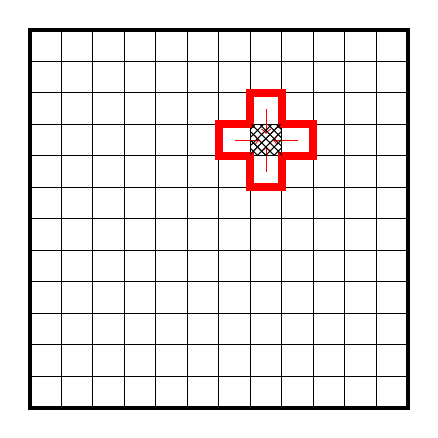
\begin{tikzpicture}[scale=0.4]
  \draw[ultra thick] (0, 0) rectangle (12, 12);
  \foreach \i in {1, 2, ..., 11} {
    \draw (\i, 0) -- +(0, 12);
    \draw (0, \i) -- +(12, 0);
  }

  \only<2>{
  \begin{scope}[xshift=2cm, yshift=2cm]
    % "croix" qui dépasse
    \draw[red, line width=1mm] (5, 5) -- ++(0, 1) -- ++ (-1, 0) -- ++(0, 1) --
    ++(1, 0) -- ++(0, 1) -- ++(1, 0) -- ++(0, -1) -- ++(1, 0) -- ++(0, -1) --
    ++(-1, 0) -- ++(0, -1) -- cycle;
    % petites flèches
    \draw[red,->] (5.5, 5.5) -- +(0, 0.8);
    \draw[red,->] (5.5, 7.5) -- +(0, -0.8);
    \draw[red,->] (4.5, 6.5) -- +(0.8, 0);
    \draw[red,->] (6.5, 6.5) -- +(-0.8, 0);
    \end{scope}
  }
    \fill<3>[pattern=crosshatch] (7, 8) rectangle +(1, 1);
\end{tikzpicture}


\end{frame}

%%%%%%%%%%%%%%%%%%%%%%%%%%%%%%%%%%%%%%%%%%%%%%%%%%%%%%%%%%%%%%%%%%%%%%

\begin{frame}
\frametitle{Décomposition de domaine}


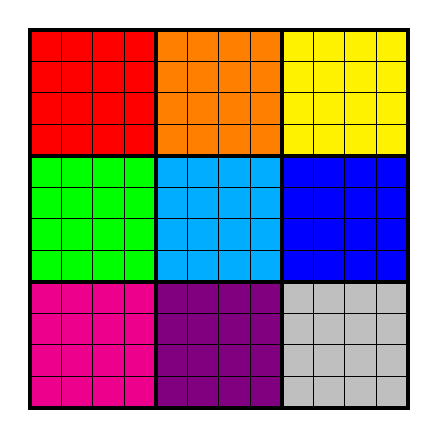
\begin{tikzpicture}[scale=0.4]
  \filldraw[very thick, fill=red]       (0, 8) rectangle  +(4, 4);
  \filldraw[very thick, fill=orange]    (4, 8) rectangle  +(4,4);
  \filldraw[very thick, fill=yellow]    (8, 8) rectangle  +(4,4);
  \filldraw[very thick, fill=green]     (0, 4) rectangle  +(4,4);
  \filldraw[very thick, fill=cyan]      (4, 4) rectangle  +(4,4);
  \filldraw[very thick, fill=blue]      (8, 4) rectangle  +(4,4);
  \filldraw[very thick, fill=magenta]   (0, 0) rectangle  +(4,4);
  \filldraw[very thick, fill=violet]    (4, 0) rectangle  +(4,4);
  \filldraw[very thick, fill=lightgray] (8, 0) rectangle  +(4,4);

  
  \draw[ultra thick] (0, 0) rectangle (12, 12);
  \foreach \i in {1, 2, ..., 11} {
    \draw (\i, 0) -- +(0, 12);
    \draw (0, \i) -- +(12, 0);
  }

  
  \end{tikzpicture}
\end{frame}

%%%%%%%%%%%%%%%%%%%%%%%%%%%%%%%%%%%%%%%%%%%%%%%%%%%%%%%%%%%%%%%%%%%%%%%%%%


\begin{frame}
\frametitle{Décomposition de domaine}


\begin{tikzpicture}[scale=0.4]
  \path[use as bounding box] (1, 0) rectangle (18, 18);
  
  % gros carrés
  \filldraw[very thick, fill=red]       (0,  14) rectangle  +(4, 4);
  \filldraw[very thick, fill=orange]    (7,  14) rectangle  +(4,4);
  \filldraw[very thick, fill=yellow]    (14, 14) rectangle  +(4,4);
  \filldraw[very thick, fill=green]     (0,  7) rectangle  +(4,4);
  \filldraw[very thick, fill=cyan]      (7,  7) rectangle  +(4,4);
  \filldraw[very thick, fill=blue]      (14, 7) rectangle  +(4,4);
  \filldraw[very thick, fill=magenta]   (0,  0) rectangle  +(4,4);
  \filldraw[very thick, fill=violet]    (7,  0) rectangle  +(4,4);
  \filldraw[very thick, fill=lightgray] (14, 0) rectangle  +(4,4);
  
  % petites cases
  \foreach \i in {0, 1, 2} {
    \foreach \j in {0, 1, 2} {
      \foreach \k in {1, 2, 3} {
        \draw (7*\i + \k, 7*\j) -- +(0, 4);
        \draw (7*\i, 7*\j + \k) -- +(4, 0);
      }
    }
  }

  \fill<4->[pattern=crosshatch] (9, 8) rectangle +(1, 1);
  \fill<3->[pattern=crosshatch] (8, 8) rectangle +(1, 1);
  
  \begin{onlyenv}<4>
      \begin{scope}[xshift=5cm, yshift=2cm]
      % "croix" qui dépasse
      \draw[red, line width=1mm] (5, 5) -- ++(0, 1) -- ++ (-1, 0) -- ++(0, 1) --
      ++(1, 0) -- ++(0, 1) -- ++(1, 0) -- ++(0, -1) -- ++(1, 0) -- ++(0, -1) --
      ++(-1, 0) -- ++(0, -1) -- cycle;
      % petites flèches
      \draw[red,->] (5.5, 5.5) -- +(0, 0.8);
      \draw[red,->] (5.5, 7.5) -- +(0, -0.8);
      \draw[red,->] (4.5, 6.5) -- +(0.8, 0);
      \draw[red,->] (6.5, 6.5) -- +(-0.8, 0);
    \end{scope}
  \end{onlyenv}
  
  \begin{onlyenv}<3>
    \begin{scope}[xshift=4cm, yshift=2cm]
      % "croix"
      \draw[red, line width=1mm] (5, 5) -- ++(0, 1) -- ++ (-1, 0) -- ++(0, 1) --
      ++(1, 0) -- ++(0, 1) -- ++(1, 0) -- ++(0, -1) -- ++(1, 0) -- ++(0, -1) --
      ++(-1, 0) -- ++(0, -1) -- cycle;
      % petites flèches
      \draw[red,->] (5.5, 5.5) -- +(0, 0.8);
      \draw[red,->] (5.5, 7.5) -- +(0, -0.8);
      \draw[red,->] (4.5, 6.5) -- +(0.8, 0);
      \draw[red,->] (6.5, 6.5) -- +(-0.8, 0);
    \end{scope}
  \end{onlyenv}
  
  \begin{onlyenv}<2>
    \begin{scope}[xshift=3cm, yshift=2cm]
      % "croix"
      \draw[red, line width=1mm] (5, 5) -- ++(0, 1) -- ++ (-1, 0) -- ++(0, 1) --
      ++(1, 0) -- ++(0, 1) -- ++(1, 0) -- ++(0, -1) -- ++(1, 0) -- ++(0, -1) --
      ++(-1, 0) -- ++(0, -1) -- cycle;
      % petites flèches
      \draw[red,->] (5.5, 5.5) -- +(0, 0.8);
      \draw[red,->] (5.5, 7.5) -- +(0, -0.8);
      \draw[red,->] (4.5, 6.5) -- +(0.8, 0);
      \draw[red,->] (6.5, 6.5) -- +(-0.8, 0);
    \end{scope}
  \end{onlyenv}
  
  \filldraw<5>[fill=blue] (11, 7) rectangle  +(1,4);
  \draw<5> (11, 8) --  +(1,0);
  \draw<5> (11, 9) --  +(1,0);
  \draw<5> (11, 10) --  +(1,0);
  \draw<5> (11, 8) --  +(1,0);
  \draw<5>[very thick]      (7,  7) rectangle  +(5,4);  
\end{tikzpicture}
\end{frame}




%%%%%%%%%%%%%%%%%%%%%%%%%%%%%%%%%%%%%%%%%%%%%%%%%%%%%%%%%%%%%%%%%%%%%%%%%%



\begin{frame}
\frametitle{Décomposition de domaine}

\begin{minipage}[T]{7.2cm}
\begin{tikzpicture}[scale=0.4]
  \path[use as bounding box] (1, 0) rectangle (18, 18);
  
  % halos
  \begin{onlyenv}<3->
  \filldraw[fill=violet]    (4, 0) rectangle  +(1,4);
  \filldraw[fill=magenta]   (6, 0) rectangle  +(1,4);
  \filldraw[fill=lightgray] (11, 0) rectangle  +(1,4);
  \filldraw[fill=violet]    (13, 0) rectangle  +(1,4);
  \filldraw[fill=cyan]    (4, 7) rectangle  +(1,4);
  \filldraw[fill=green]   (6, 7) rectangle  +(1,4);
  \filldraw[fill=blue] (11, 7) rectangle  +(1,4);
  \filldraw[fill=cyan]    (13, 7) rectangle  +(1,4);
  \filldraw[fill=orange]    (4, 14) rectangle  +(1,4);
  \filldraw[fill=red]   (6, 14) rectangle  +(1,4);
  \filldraw[fill=yellow]    (11,14) rectangle  +(1,4);
  \filldraw[fill=orange]    (13,14) rectangle  +(1,4);
  
  \filldraw[fill=blue]      (14, 4) rectangle  +(4,1);
  \filldraw[fill=cyan]      (7, 4) rectangle  +(4,1);
  \filldraw[fill=green]      (0, 4) rectangle  +(4,1);
  \filldraw[fill=lightgray]   (14, 6) rectangle  +(4,1);
  \filldraw[fill=violet]      (7, 6) rectangle  +(4,1);
  \filldraw[fill=magenta]     (0, 6) rectangle  +(4,1);  
  \filldraw[fill=blue]      (14, 13) rectangle  +(4,1);
  \filldraw[fill=cyan]      (7, 13) rectangle  +(4,1);
  \filldraw[fill=green]      (0, 13) rectangle  +(4,1);
  \filldraw[fill=yellow]      (14, 11) rectangle  +(4,1);
  \filldraw[fill=orange]      (7, 11) rectangle  +(4,1);
  \filldraw[fill=red]      (0, 11) rectangle  +(4,1);
\end{onlyenv}

  % gros carrés
    \filldraw[very thick, fill=red]       (0,  14) rectangle  +(4, 4);
    \filldraw[very thick, fill=orange]    (7,  14) rectangle  +(4,4);
    \filldraw[very thick, fill=yellow]    (14, 14) rectangle  +(4,4);
    \filldraw[very thick, fill=green]     (0,  7) rectangle  +(4,4);
    \filldraw[very thick, fill=cyan]      (7,  7) rectangle  +(4,4);
    \filldraw[very thick, fill=blue]      (14, 7) rectangle  +(4,4);
    \filldraw[very thick, fill=magenta]   (0,  0) rectangle  +(4,4);
    \filldraw[very thick, fill=violet]    (7,  0) rectangle  +(4,4);
    \filldraw[very thick, fill=lightgray] (14, 0) rectangle  +(4,4);
  
  \begin{onlyenv}<4->
    \draw[pattern=crosshatch, pattern color=black, very thick]       (0,  14) rectangle  +(4, 4);
    \draw[pattern=crosshatch, pattern color=black, very thick]    (7,  14) rectangle  +(4,4);
    \draw[pattern=crosshatch, pattern color=black, very thick]    (14, 14) rectangle  +(4,4);
    \draw[pattern=crosshatch, pattern color=black, very thick]     (0,  7) rectangle  +(4,4);
    \draw[pattern=crosshatch, pattern color=black, very thick]      (7,  7) rectangle  +(4,4);
    \draw[pattern=crosshatch, pattern color=black, very thick]      (14, 7) rectangle  +(4,4);
    \draw[pattern=crosshatch, pattern color=black, very thick]   (0,  0) rectangle  +(4,4);
    \draw[pattern=crosshatch, pattern color=black, very thick]    (7,  0) rectangle  +(4,4);
    \draw[pattern=crosshatch, pattern color=black, very thick] (14, 0) rectangle  +(4,4);
  \end{onlyenv}
  
  % hachures

  % petites cases, sans halo
  \begin{onlyenv}<1-2>
    \foreach \i in {0, 1, 2} {
      \foreach \j in {0, 1, 2} {
        \foreach \k in {1, 2, 3} {
          \draw (7*\i + \k, 7*\j) -- +(0, 4);
          \draw (7*\i, 7*\j + \k) -- +(4, 0);
        }
      }
    }
  \end{onlyenv}

  \begin{onlyenv}<3->
  % petites cases, halos compris
  \foreach \k in {1, 2, 3} {
    \draw (\k, 0) -- +(0, 5);
    \draw (0, \k) -- +(5, 0);
  }
  \foreach \k in {1, 2, 3} {
    \draw (\k, 6) -- +(0, 6);
    \draw (0, 7 + \k) -- +(5, 0);
  }
  \foreach \k in {1, 2, 3, 4} {
    \draw (\k, 13) -- +(0, 5);
    \draw (0, 13 + \k) -- +(5, 0);
  }
  \foreach \k in {1, 2, 3} {
    \draw (7 + \k, 0) -- +(0, 5);
    \draw (6, \k) -- +(6, 0);
  }
  \foreach \k in {1, 2, 3} {
    \draw (7 + \k, 6) -- +(0, 6);
    \draw (6, 7 + \k) -- +(6, 0);
  }
  \foreach \k in {1, 2, 3} {
    \draw (7 + \k, 13) -- +(0, 5);
    \draw (6, 14 + \k) -- +(6, 0);
  }
  \foreach \k in {1, 2, 3} {
    \draw (14 + \k, 0) -- +(0, 5);
    \draw (13, \k) -- +(5, 0);
  }
  \foreach \k in {1, 2, 3} {
    \draw (14 + \k, 6) -- +(0, 6);
    \draw (13, 7 + \k) -- +(5, 0);
  }
  \foreach \k in {1, 2, 3} {
    \draw (14 + \k, 13) -- +(0, 5);
    \draw (13, 14 + \k) -- +(5, 0);
  }
\end{onlyenv}

% flèches des halos
  \begin{onlyenv}<2,5>
 \begin{scope}[xshift=0cm, yshift=14cm]
   \draw[red, ultra thick, ->] (3.5, 0) to[bend right=20mm] +(2.5, 0);
   \draw[red, ultra thick, ->] (0, 0.5) to[bend right=20mm] +(0, -2.5);
 \end{scope}
 \begin{scope}[xshift=7cm, yshift=14cm]
   \draw[orange, ultra thick, ->] (3.5, 0) to[bend right=20mm] +(2.5, 0);
   \draw[orange, ultra thick, ->] (0.5, 4) to[bend right=20mm] +(-2.5, 0);
   \draw[orange, ultra thick, ->] (0, 0.5) to[bend right=20mm] +(0, -2.5);
 \end{scope}
 \begin{scope}[xshift=14cm, yshift=14cm]
   \draw[yellow, ultra thick, ->] (0.5, 4) to[bend right=20mm] +(-2.5, 0);
   \draw[yellow, ultra thick, ->] (0, 0.5) to[bend right=20mm] +(0, -2.5);
 \end{scope}

 \begin{scope}[xshift=0cm, yshift=7cm]
 \draw[green, ultra thick, ->] (3.5, 0) to[bend right=20mm] +(2.5, 0);
 \draw[green, ultra thick, ->] (0, 0.5) to[bend right=20mm] +(0, -2.5);
 \draw[green, ultra thick, ->] (4, 3.5) to[bend right=20mm] +(0, 2.5);
\end{scope}
 \begin{scope}[xshift=7cm, yshift=7cm]
 \draw[cyan, ultra thick, ->] (3.5, 0) to[bend right=20mm] +(2.5, 0);
 \draw[cyan, ultra thick, ->] (0.5, 4) to[bend right=20mm] +(-2.5, 0);
 \draw[cyan, ultra thick, ->] (0, 0.5) to[bend right=20mm] +(0, -2.5);
 \draw[cyan, ultra thick, ->] (4, 3.5) to[bend right=20mm] +(0, 2.5);
\end{scope}
  \begin{scope}[xshift=14cm, yshift=7cm]
 \draw[blue, ultra thick, ->] (0.5, 4) to[bend right=20mm] +(-2.5, 0);
 \draw[blue, ultra thick, ->] (0, 0.5) to[bend right=20mm] +(0, -2.5);
 \draw[blue, ultra thick, ->] (4, 3.5) to[bend right=20mm] +(0, 2.5);
\end{scope}
 \begin{scope}[xshift=0cm, yshift=0cm]
 \draw[magenta, ultra thick, ->] (3.5, 0) to[bend right=20mm] +(2.5, 0);
 \draw[magenta, ultra thick, ->] (4, 3.5) to[bend right=20mm] +(0, 2.5);
\end{scope}
 \begin{scope}[xshift=7cm, yshift=0cm]
 \draw[violet, ultra thick, ->] (3.5, 0) to[bend right=20mm] +(2.5, 0);
 \draw[violet, ultra thick, ->] (0.5, 4) to[bend right=20mm] +(-2.5, 0);
 \draw[violet, ultra thick, ->] (4, 3.5) to[bend right=20mm] +(0, 2.5);
\end{scope}
  \begin{scope}[xshift=14cm, yshift=0cm]
 \draw[lightgray, ultra thick, ->] (0.5, 4) to[bend right=20mm] +(-2.5, 0);
 \draw[lightgray, ultra thick, ->] (4, 3.5) to[bend right=20mm] +(0, 2.5);
\end{scope}
\end{onlyenv}

\end{tikzpicture}%
\end{minipage}\begin{minipage}[T]{4.5cm}
  Chaque processeur :
  \medskip
  \begin{itemize}
  \item<1-> connaît $T$ à l'instant~$t$.
  \item<2-> envoie/reçoit le \alert{halo} de ses voisins.
  \item<4-> calcule $T$ à l'instant $t + \Delta t$.
  \item<5-> recommencer...
  \end{itemize}

  \medskip

  \begin{alertblock}<6>{Problème}
    Calculs bloqués par les communications
  \end{alertblock}
\end{minipage}
\end{frame}


%%%%%%%%%%%%%%%%%%%%%%%%%%%%%%%%%%%%%%%%

\begin{frame}
\frametitle{Décomposition de domaine}

\begin{minipage}[T]{7.2cm}
\begin{tikzpicture}[scale=0.4]
  \path[use as bounding box] (1, 0) rectangle (18, 18);
  
  % halos
  \begin{onlyenv}<4->
  \filldraw[fill=violet]    (4, 0) rectangle  +(1,4);
  \filldraw[fill=magenta]   (6, 0) rectangle  +(1,4);
  \filldraw[fill=lightgray] (11, 0) rectangle  +(1,4);
  \filldraw[fill=violet]    (13, 0) rectangle  +(1,4);
  \filldraw[fill=cyan]    (4, 7) rectangle  +(1,4);
  \filldraw[fill=green]   (6, 7) rectangle  +(1,4);
  \filldraw[fill=blue] (11, 7) rectangle  +(1,4);
  \filldraw[fill=cyan]    (13, 7) rectangle  +(1,4);
  \filldraw[fill=orange]    (4, 14) rectangle  +(1,4);
  \filldraw[fill=red]   (6, 14) rectangle  +(1,4);
  \filldraw[fill=yellow]    (11,14) rectangle  +(1,4);
  \filldraw[fill=orange]    (13,14) rectangle  +(1,4);
  
  \filldraw[fill=blue]      (14, 4) rectangle  +(4,1);
  \filldraw[fill=cyan]      (7, 4) rectangle  +(4,1);
  \filldraw[fill=green]      (0, 4) rectangle  +(4,1);
  \filldraw[fill=lightgray]   (14, 6) rectangle  +(4,1);
  \filldraw[fill=violet]      (7, 6) rectangle  +(4,1);
  \filldraw[fill=magenta]     (0, 6) rectangle  +(4,1);  
  \filldraw[fill=blue]      (14, 13) rectangle  +(4,1);
  \filldraw[fill=cyan]      (7, 13) rectangle  +(4,1);
  \filldraw[fill=green]      (0, 13) rectangle  +(4,1);
  \filldraw[fill=yellow]      (14, 11) rectangle  +(4,1);
  \filldraw[fill=orange]      (7, 11) rectangle  +(4,1);
  \filldraw[fill=red]      (0, 11) rectangle  +(4,1);
\end{onlyenv}

  % gros carrés
    \filldraw[very thick, fill=red]       (0,  14) rectangle  +(4, 4);
    \filldraw[very thick, fill=orange]    (7,  14) rectangle  +(4,4);
    \filldraw[very thick, fill=yellow]    (14, 14) rectangle  +(4,4);
    \filldraw[very thick, fill=green]     (0,  7) rectangle  +(4,4);
    \filldraw[very thick, fill=cyan]      (7,  7) rectangle  +(4,4);
    \filldraw[very thick, fill=blue]      (14, 7) rectangle  +(4,4);
    \filldraw[very thick, fill=magenta]   (0,  0) rectangle  +(4,4);
    \filldraw[very thick, fill=violet]    (7,  0) rectangle  +(4,4);
    \filldraw[very thick, fill=lightgray] (14, 0) rectangle  +(4,4);
  
  \begin{onlyenv}<3-4>
    \draw[pattern=crosshatch, pattern color=black, very thick]    (1,  15) rectangle  +(2, 2);
    \draw[pattern=crosshatch, pattern color=black, very thick]    (8,  15) rectangle +(2, 2);
    \draw[pattern=crosshatch, pattern color=black, very thick]    (15, 15) rectangle +(2, 2);
    \draw[pattern=crosshatch, pattern color=black, very thick]    (1,  8) rectangle  +(2, 2);
    \draw[pattern=crosshatch, pattern color=black, very thick]    (8,  8) rectangle  +(2, 2);
    \draw[pattern=crosshatch, pattern color=black, very thick]    (15, 8) rectangle  +(2, 2);
    \draw[pattern=crosshatch, pattern color=black, very thick]    (1,  1) rectangle  +(2, 2);
    \draw[pattern=crosshatch, pattern color=black, very thick]    (8,  1) rectangle  +(2, 2);
    \draw[pattern=crosshatch, pattern color=black, very thick]    (15, 1) rectangle  +(2, 2);
  \end{onlyenv}

    \begin{onlyenv}<5->
    \draw[pattern=crosshatch, pattern color=black, very thick]       (0,  14) rectangle  +(4, 4);
    \draw[pattern=crosshatch, pattern color=black, very thick]    (7,  14) rectangle  +(4,4);
    \draw[pattern=crosshatch, pattern color=black, very thick]    (14, 14) rectangle  +(4,4);
    \draw[pattern=crosshatch, pattern color=black, very thick]     (0,  7) rectangle  +(4,4);
    \draw[pattern=crosshatch, pattern color=black, very thick]      (7,  7) rectangle  +(4,4);
    \draw[pattern=crosshatch, pattern color=black, very thick]      (14, 7) rectangle  +(4,4);
    \draw[pattern=crosshatch, pattern color=black, very thick]   (0,  0) rectangle  +(4,4);
    \draw[pattern=crosshatch, pattern color=black, very thick]    (7,  0) rectangle  +(4,4);
    \draw[pattern=crosshatch, pattern color=black, very thick] (14, 0) rectangle  +(4,4);
  \end{onlyenv}
  
  % hachures

  % petites cases, sans halo
  \begin{onlyenv}<1-3>
    \foreach \i in {0, 1, 2} {
      \foreach \j in {0, 1, 2} {
        \foreach \k in {1, 2, 3} {
          \draw (7*\i + \k, 7*\j) -- +(0, 4);
          \draw (7*\i, 7*\j + \k) -- +(4, 0);
        }
      }
    }
  \end{onlyenv}

  \begin{onlyenv}<4->
  % petites cases, halos compris
  \foreach \k in {1, 2, 3} {
    \draw (\k, 0) -- +(0, 5);
    \draw (0, \k) -- +(5, 0);
  }
  \foreach \k in {1, 2, 3} {
    \draw (\k, 6) -- +(0, 6);
    \draw (0, 7 + \k) -- +(5, 0);
  }
  \foreach \k in {1, 2, 3, 4} {
    \draw (\k, 13) -- +(0, 5);
    \draw (0, 13 + \k) -- +(5, 0);
  }
  \foreach \k in {1, 2, 3} {
    \draw (7 + \k, 0) -- +(0, 5);
    \draw (6, \k) -- +(6, 0);
  }
  \foreach \k in {1, 2, 3} {
    \draw (7 + \k, 6) -- +(0, 6);
    \draw (6, 7 + \k) -- +(6, 0);
  }
  \foreach \k in {1, 2, 3} {
    \draw (7 + \k, 13) -- +(0, 5);
    \draw (6, 14 + \k) -- +(6, 0);
  }
  \foreach \k in {1, 2, 3} {
    \draw (14 + \k, 0) -- +(0, 5);
    \draw (13, \k) -- +(5, 0);
  }
  \foreach \k in {1, 2, 3} {
    \draw (14 + \k, 6) -- +(0, 6);
    \draw (13, 7 + \k) -- +(5, 0);
  }
  \foreach \k in {1, 2, 3} {
    \draw (14 + \k, 13) -- +(0, 5);
    \draw (13, 14 + \k) -- +(5, 0);
  }
\end{onlyenv}

% flèches des halos
  \begin{onlyenv}<2-3,6>
 \begin{scope}[xshift=0cm, yshift=14cm]
   \draw[red, ultra thick, ->] (3.5, 0) to[bend right=20mm] +(2.5, 0);
   \draw[red, ultra thick, ->] (0, 0.5) to[bend right=20mm] +(0, -2.5);
 \end{scope}
 \begin{scope}[xshift=7cm, yshift=14cm]
   \draw[orange, ultra thick, ->] (3.5, 0) to[bend right=20mm] +(2.5, 0);
   \draw[orange, ultra thick, ->] (0.5, 4) to[bend right=20mm] +(-2.5, 0);
   \draw[orange, ultra thick, ->] (0, 0.5) to[bend right=20mm] +(0, -2.5);
 \end{scope}
 \begin{scope}[xshift=14cm, yshift=14cm]
   \draw[yellow, ultra thick, ->] (0.5, 4) to[bend right=20mm] +(-2.5, 0);
   \draw[yellow, ultra thick, ->] (0, 0.5) to[bend right=20mm] +(0, -2.5);
 \end{scope}

 \begin{scope}[xshift=0cm, yshift=7cm]
 \draw[green, ultra thick, ->] (3.5, 0) to[bend right=20mm] +(2.5, 0);
 \draw[green, ultra thick, ->] (0, 0.5) to[bend right=20mm] +(0, -2.5);
 \draw[green, ultra thick, ->] (4, 3.5) to[bend right=20mm] +(0, 2.5);
\end{scope}
 \begin{scope}[xshift=7cm, yshift=7cm]
 \draw[cyan, ultra thick, ->] (3.5, 0) to[bend right=20mm] +(2.5, 0);
 \draw[cyan, ultra thick, ->] (0.5, 4) to[bend right=20mm] +(-2.5, 0);
 \draw[cyan, ultra thick, ->] (0, 0.5) to[bend right=20mm] +(0, -2.5);
 \draw[cyan, ultra thick, ->] (4, 3.5) to[bend right=20mm] +(0, 2.5);
\end{scope}
  \begin{scope}[xshift=14cm, yshift=7cm]
 \draw[blue, ultra thick, ->] (0.5, 4) to[bend right=20mm] +(-2.5, 0);
 \draw[blue, ultra thick, ->] (0, 0.5) to[bend right=20mm] +(0, -2.5);
 \draw[blue, ultra thick, ->] (4, 3.5) to[bend right=20mm] +(0, 2.5);
\end{scope}
 \begin{scope}[xshift=0cm, yshift=0cm]
 \draw[magenta, ultra thick, ->] (3.5, 0) to[bend right=20mm] +(2.5, 0);
 \draw[magenta, ultra thick, ->] (4, 3.5) to[bend right=20mm] +(0, 2.5);
\end{scope}
 \begin{scope}[xshift=7cm, yshift=0cm]
 \draw[violet, ultra thick, ->] (3.5, 0) to[bend right=20mm] +(2.5, 0);
 \draw[violet, ultra thick, ->] (0.5, 4) to[bend right=20mm] +(-2.5, 0);
 \draw[violet, ultra thick, ->] (4, 3.5) to[bend right=20mm] +(0, 2.5);
\end{scope}
  \begin{scope}[xshift=14cm, yshift=0cm]
 \draw[lightgray, ultra thick, ->] (0.5, 4) to[bend right=20mm] +(-2.5, 0);
 \draw[lightgray, ultra thick, ->] (4, 3.5) to[bend right=20mm] +(0, 2.5);
\end{scope}
\end{onlyenv}

\end{tikzpicture}%
\end{minipage}\begin{minipage}[T]{4.5cm}
  Chaque processeur :
  \medskip
  \begin{itemize}
  \item<1-> connaît $T$ à l'instant~$t$.
  \item<2-> envoie le \alert{halo} à ses voisins (\alert{Isend}) .
  \item<3-> calcule $T$ à l'instant $t + \Delta t$ \alert{à l'intérieur}.
  \item<4-> attend fin des comms
  \item<5-> calcule $T$ à l'instant $t + \Delta t$ \alert{sur les bords}.
  \item<6-> recommencer...
  \end{itemize}
\end{minipage}
\end{frame}

%%%%%%%%%%%%%%%%%%%%%%%

\begin{frame}[fragile]
%\frametitle{Concrètement}

Bloquant :
\begin{minted}[fontsize=\footnotesize]{C}
int MPI_Sendrecv(void *sendbuf, int sendcount, MPI_Datatype sendtype, 
                 int dest, int sendtag, 
                 void *recvbuf, int recvcount, MPI_Datatype recvtype, 
                 int source, int recvtag, 
                 MPI_Comm comm, MPI_Status *status);
\end{minted}

Non-bloquant :
\begin{minted}[fontsize=\footnotesize]{C}
int MPI_Isend(void *buf, int count, MPI_Datatype datatype, 
              int dest, int tag, 
              MPI_Comm comm, MPI_Request *request);
int MPI_Irecv(void *buf, int count, MPI_Datatype datatype,
              int source, int tag, 
              MPI_Comm comm, MPI_Request *request);
int MPI_Waitall(int count, 
                MPI_Request requests[], MPI_Status statuses[]);
\end{minted}

\begin{alertblock}{Attention !}
  \begin{itemize}    
  \item Bord est / ouest : données \alert{non-contigües} en mémoire !
    \item[$\Rightarrow$] création de \alert{types MPI dérivés} (\mintinline{C}{MPI_Type_vector(...)})
  \end{itemize}
\end{alertblock}
\end{frame}

%%%%%%%%%%%%%%%%%%%%%%%

\end{document}

\section{Généralités}

%%%%%%%%%%%%%%%%%%%%%%%%%%%%%%%%%%%%%%%%%%%%%%%%%%%%%%%%%%%%%%%%%%%%%%
\begin{frame}
\frametitle{How to write an effective parallel program?}

\begin{block}{First Principles}

\begin{itemize}
\item {\bf location of data} : {\it Carefully organize the data so that each processor
    maximizes the amount of data in their reach.}

\medskip

\item {\bf load balancing} : {\it minimize periods of inactivity by taking into account
    the unique characteristics of each processor and assigning work accordingly.}

\medskip

\item {\bf recouvrement des communications par le calcul} : {\it Avoid having processors
    sit idle during communicating transfers.}
\end{itemize}
\end{block}

\end{frame}


%%%%%%%%%%%%%%%%%%%%%%%%%%%%%%%%%%%%%%%%%%%%%%%%%%%%%%%%%%%%%%%%%%%%%%
\begin{frame}
\frametitle{Load balancing}


\begin{exampleblock}{Predictable workload}

  \begin{itemize}
  \item[$\Rightarrow$] \textbf{static} workload.

  \item All data requiring the same amount of calculation time.

    $\rightarrow$ Distributed by block, cyclic, \dots

  \item Regular data with different calculation time

    $\rightarrow$ use of a cost function $+$ block distribution,
    cyclic, \dots

\end{itemize}
\end{exampleblock}

\medskip

\begin{alertblock}{Unpredictable workload}
  \begin{itemize}
   \item[$\Rightarrow$]  \textbf{dynamic} load balancing
   \item \sout{master-slave} boss-worker model
   \item self-regulating model (\og work stealing\fg)
   \end{itemize}
 \end{alertblock}


\end{frame}


%%%%%%%%%%%%%%%%%%%%%%%%%%%%%%%%%%%%%%%%%%%%%%%%%%%%%%%%%%%%%%%%%%%%%%
\begin{frame}
\frametitle{Boss-Worker \sout{master-slave} Model}


\begin{itemize}
\item The boss knows the data and the work to be done
\item Available workers ask for work
\item The boss either provides a task to do or orders the workers to stop
\begin{alertblock}{Limitations}
\begin{itemize}
\item The boss needs a lot of RAM if he's in charge of all the data
\item 2 message exchanges per task (A/R) $\longrightarrow$ high granularity
\item Too many workers $\rightarrow$ the boss becomes a bottleneck
\end{itemize}
\end{alertblock}

\begin{exampleblock}{Advantages~:}
\begin{itemize}
\item load balancing, even with heterogenous resources (or availability/speed that varies with time)
\item very easy \emph{checkpointing} (only the boss)
\end{itemize}
\end{exampleblock}

\end{itemize}

\end{frame}


%%%%%%%%%%%%%%%%%%%%%%%%%%%%%%%%%%%%%%%%%%%%%%%%%%%%%%%%%%%%%%%%%%%%%%
\begin{frame}
\frametitle{Self-Regulating Model}

\begin{exampleblock}{Work stealing principle}

\begin{itemize}
\item Each processor manages their own list of work to do

  \begin{itemize}
  \item Initial distribution assumed to be equal
  \end{itemize}

\item If the task list is empty :
  \begin{itemize}
  \item Choose a \emph{victim} (randomly?)
  \item \og Steal \fg a fraction (50\% ?) of the victim's remaining work
  \end{itemize}
\end{itemize}
\end{exampleblock}

\bigskip

\begin{itemize}
\item [+] Completely symmetrical
  \begin{itemize}
  \item No god nor master \CircledA
  \end{itemize}

\item [+] Every process participates in the calculation
  \begin{itemize}
  \item No \sout{parasitic} bosses twiddling their thumbs

  \end{itemize}
\item [--] not easy to detect when there's no more work to do
\item [--] difficult to program
\item [--] difficult to establish \emph{checkpointing}
\end{itemize}

\end{frame}



%%%%%%%%%%%%%%%%%%%%%%%%%%%%%%%%%%%%%%%%%%%%%%%%%%%%%%%%%%%%%%%%%%%%%

\begin{frame}[fragile]
\frametitle{Parallélisme de données}


\begin{block}{Exemple classique : \emph{map}}
\begin{minted}{C}
for (int i = 0; i < n; i++)
    B[i] = f(A[i], i)
\end{minted}
\end{block}

\bigskip

\begin{itemize}
\item Pas besoin de communication / synchronisation !
\item Répartition des données ?
\item Équilibrage de charge
\end{itemize}
\end{frame}

%%%%%%%%%%%%%%%%%%%%%%%%%%%%%%%%%%%%%%%%%%%%%%%%%%%%%%%%%%%%%%%%%

\section{Distribution de données}

\begin{frame}
\frametitle{Répartition 1D}

Par blocs :

\medskip

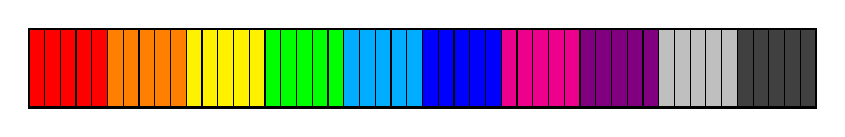
\begin{tikzpicture}
  \filldraw[fill=red]    (0, 0) rectangle  +(1,1);
  \filldraw[fill=orange] (1, 0) rectangle  +(1,1);
  \filldraw[fill=yellow] (2, 0) rectangle  +(1,1);
  \filldraw[fill=green]  (3, 0) rectangle  +(1,1);
  \filldraw[fill=cyan]   (4, 0) rectangle  +(1,1);
  \filldraw[fill=blue]   (5, 0) rectangle  +(1,1);
  \filldraw[fill=magenta] (6, 0) rectangle  +(1,1);
  \filldraw[fill=violet] (7, 0) rectangle +(1,1);
  \filldraw[fill=lightgray] (8, 0) rectangle +(1,1);
  \filldraw[fill=darkgray] (9, 0) rectangle +(1,1);
  
  \draw[thick] (0, 0) rectangle (10, 1);
  \foreach \i in {0.2, 0.4, ..., 9.8}
  \draw (\i, 0) -- +(0, 1);
\end{tikzpicture}

\begin{itemize}
\item Le plus simple !
\item Favorisé par MPI
\end{itemize}

\vspace{1cm}

Cyclique :

\medskip

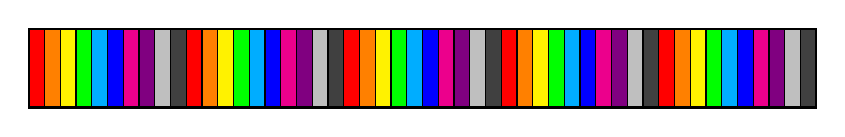
\begin{tikzpicture}
  \foreach \i in {0, 2, 4, 6, 8} {
    \filldraw[fill=red]    (\i, 0) rectangle  +(0.2,1);
    \filldraw[fill=orange]    (\i + 0.2, 0) rectangle  +(0.2,1);
    \filldraw[fill=yellow]    (\i + 0.4, 0) rectangle  +(0.2,1);
    \filldraw[fill=green]    (\i + 0.6, 0) rectangle  +(0.2,1);
    \filldraw[fill=cyan]    (\i + 0.8, 0) rectangle  +(0.2,1);
    \filldraw[fill=blue]    (\i + 1, 0) rectangle  +(0.2,1);
    \filldraw[fill=magenta]    (\i + 1.2, 0) rectangle  +(0.2,1);
    \filldraw[fill=violet]    (\i + 1.4, 0) rectangle  +(0.2,1);
    \filldraw[fill=lightgray]    (\i + 1.6, 0) rectangle  +(0.2,1);
    \filldraw[fill=darkgray]    (\i + 1.8, 0) rectangle  +(0.2,1);
  }
  % \filldraw[fill=red]    (0, 0) rectangle  +(1,1);
  % \filldraw[fill=orange] (1, 0) rectangle  +(1,1);
  % \filldraw[fill=yellow] (2, 0) rectangle  +(1,1);
  % \filldraw[fill=green]  (3, 0) rectangle  +(1,1);
  % \filldraw[fill=cyan]   (4, 0) rectangle  +(1,1);
  % \filldraw[fill=blue]   (5, 0) rectangle  +(1,1);
  % \filldraw[fill=magenta] (6, 0) rectangle  +(1,1);
  % \filldraw[fill=violet] (7, 0) rectangle +(1,1);
  % \filldraw[fill=lightgray] (8, 0) rectangle +(1,1);
  % \filldraw[fill=darkgray] (9, 0) rectangle +(1,1);
  
  \draw[thick] (0, 0) rectangle (10, 1);
  \foreach \i in {0.2, 0.4, ..., 9.8}
  \draw (\i, 0) -- +(0, 1);
\end{tikzpicture}

\begin{itemize}
\item Améliore parfois l'équilibrage de charge.
\item Possible aussi avec MPI (\texttt{MPI\_Type\_vector}...)
\end{itemize}
\end{frame}

%%%%%%%%%%%%%%%%%%%%%%%%%%%%%%%%%%%%%%%%%%%%%%%%%%%%

\begin{frame}
\frametitle{Répartition 1D (de données 2D)}

Par blocs :

\medskip

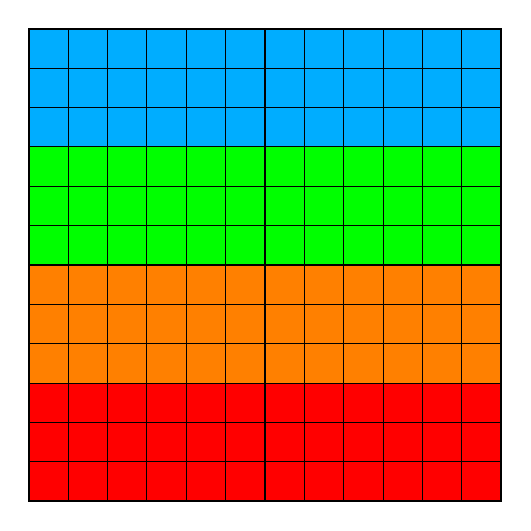
\begin{tikzpicture}[scale=0.5]
  \filldraw[fill=red]    (0, 0) rectangle  +(12,3);
  \filldraw[fill=orange] (0, 3) rectangle  +(12,3);
  \filldraw[fill=green] (0, 6) rectangle  +(12,3);
  \filldraw[fill=cyan]  (0, 9) rectangle  +(12,3);
  
  \draw[thick] (0, 0) rectangle (12, 12);
  \foreach \i in {1, 2, ..., 11} {
    \draw (\i, 0) -- +(0, 12);
    \draw (0, \i) -- +(12, 0);
  }
\end{tikzpicture}
\end{frame}


%%%%%%%%%%%%%%%%%%%%%%%%%%%%%%%%%%%%%%%%%%%%%%%%%%%%

\begin{frame}
\frametitle{Répartition 1D (de données 2D)}

Cyclique :

\medskip

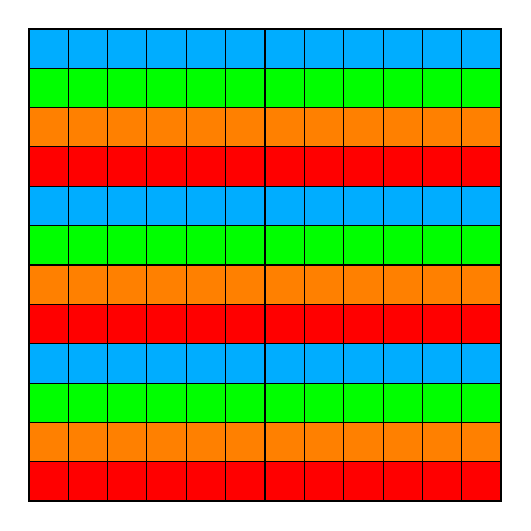
\begin{tikzpicture}[scale=0.5]
  \foreach \i in {0, 4, 8} {
    \filldraw[fill=red]    (0, \i) rectangle  +(12,1);
    \filldraw[fill=orange] (0, 1+\i) rectangle  +(12,1);
    \filldraw[fill=green] (0, 2+\i) rectangle  +(12,1);
    \filldraw[fill=cyan]  (0, 3+\i) rectangle  +(12,1);
  }
  \draw[thick] (0, 0) rectangle (12, 12);
  \foreach \i in {1, 2, ..., 11} {
    \draw (\i, 0) -- +(0, 12);
    \draw (0, \i) -- +(12, 0);
  }
\end{tikzpicture}
\end{frame}

%%%%%%%%%%%%%%%%%%%%%%%%%%%%%%%%

\begin{frame}
\frametitle{Répartition 2D (de données 2D)}

Par blocs :

\medskip

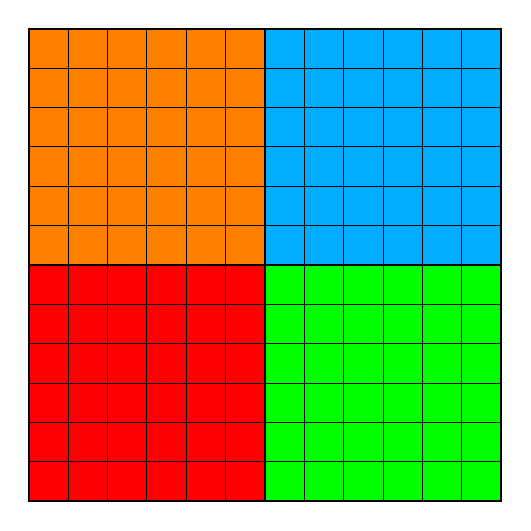
\begin{tikzpicture}[scale=0.5]
  \filldraw[fill=red]    (0, 0) rectangle  +(6, 6);
  \filldraw[fill=orange] (0, 6) rectangle  +(6,6);
  \filldraw[fill=green] (6, 0) rectangle  +(6,6);
  \filldraw[fill=cyan]  (6, 6) rectangle  +(6,6);

  \draw[thick] (0, 0) rectangle (12, 12);
  \foreach \i in {1, 2, ..., 11} {
    \draw (\i, 0) -- +(0, 12);
    \draw (0, \i) -- +(12, 0);
  }
\end{tikzpicture}
\end{frame}

%%%%%%%%%%

\begin{frame}
\frametitle{Répartition 2D (de données 2D)}

Cyclique :

\medskip

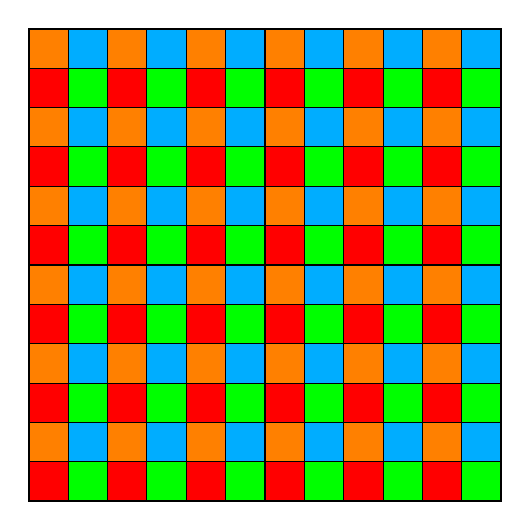
\begin{tikzpicture}[scale=0.5]
  \foreach \i in {0, 2, 4, 6, 8, 10} {
    \foreach \j in {0, 2, 4, 6, 8, 10} {
      \filldraw[fill=red]    (\i, \j) rectangle  +(1, 1);
      \filldraw[fill=orange] (\i, 1+\j) rectangle  +(1,1);
      \filldraw[fill=green] (\i+1, \j) rectangle  +(1,1);
      \filldraw[fill=cyan]  (\i+1, 1+\j) rectangle  +(1,1);
    }
  }
  \draw[thick] (0, 0) rectangle (12, 12);
  \foreach \i in {1, 2, ..., 11} {
    \draw (\i, 0) -- +(0, 12);
    \draw (0, \i) -- +(12, 0);
  }
\end{tikzpicture}
\end{frame}

%%%%%%%%%%%%%%%%%%%%%%%%

\begin{frame}
\frametitle{Répartition 1D (de données 3D)}

\centering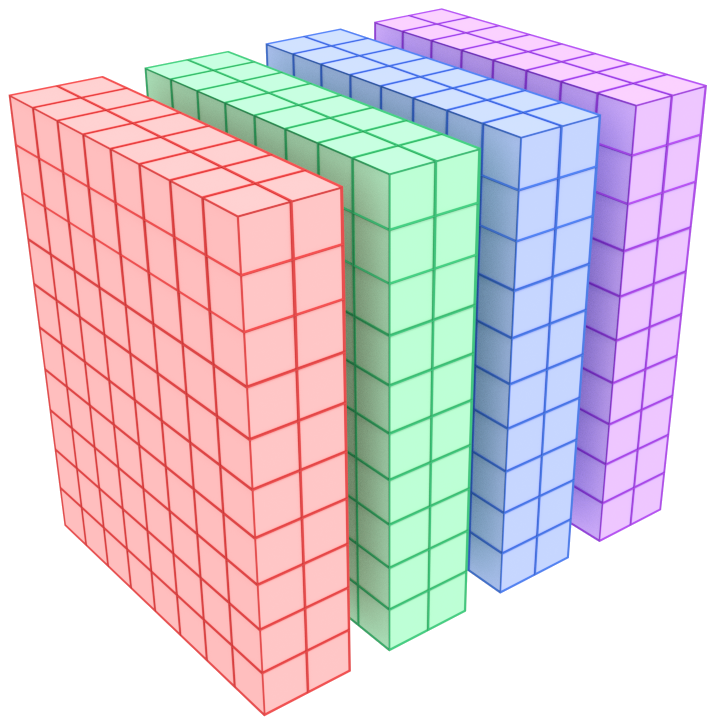
\includegraphics[height=8cm]{slabs.png}

\end{frame}

%%%%%%%%%%%%%%%%%%%%%%%%

\begin{frame}
\frametitle{Répartition 2D (de données 3D)}

\centering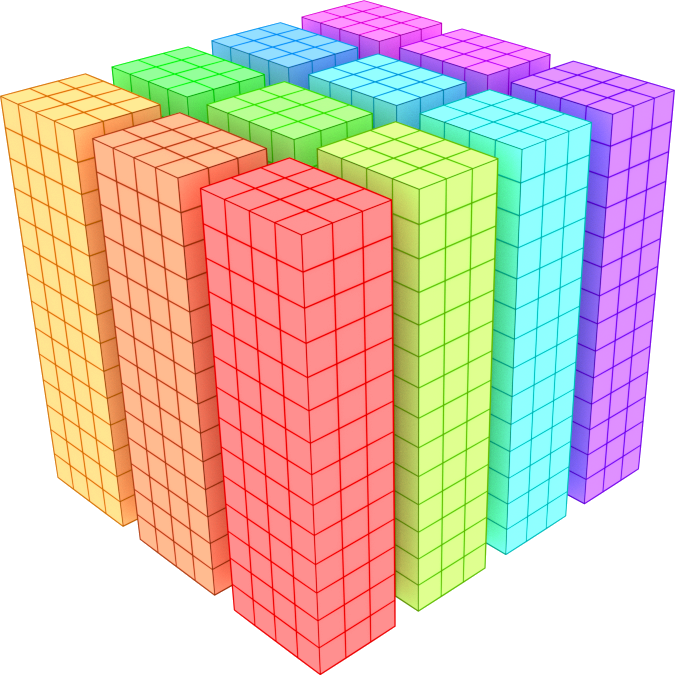
\includegraphics[height=8cm]{pencils.png}

\end{frame}

%%%%%%%%%%%%%%%%%%%%%%%%%

\section{Algos et coût des opérations collectives}

\begin{frame}[fragile]
\frametitle{Parallélisme de données}


\begin{block}{Exemple classique : \emph{reduce}}
\begin{minted}{C}
sum = 0
for (int i = 0; i < n; i++)
    sum = sum + A[i]
\end{minted}
\end{block}

\bigskip

\begin{itemize}
\item Mémoire distribuée $\rightarrow$ communications
\item Algorithme \og classique\fg en arbre.
\end{itemize}
\end{frame}

%%%%%%%%%%%%%%%%%%%%%%%%%%%%%%%%%%%%%%%%%%%%%%%%%%%%%%%%%%%%%%%%

\begin{frame}
\frametitle{Algorithme (mémoire partagée) pour \texttt{reduce}}

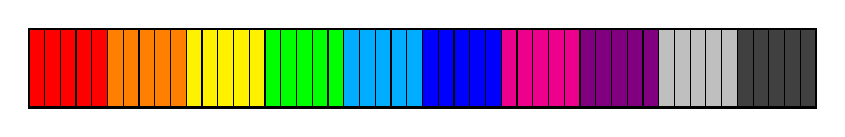
\begin{tikzpicture}
  \filldraw[fill=red]    (0, 0) rectangle  +(1,1);
  \filldraw[fill=orange] (1, 0) rectangle  +(1,1);
  \filldraw[fill=yellow] (2, 0) rectangle  +(1,1);
  \filldraw[fill=green]  (3, 0) rectangle  +(1,1);
  \filldraw[fill=cyan]   (4, 0) rectangle  +(1,1);
  \filldraw[fill=blue]   (5, 0) rectangle  +(1,1);
  \filldraw[fill=magenta] (6, 0) rectangle  +(1,1);
  \filldraw[fill=violet] (7, 0) rectangle +(1,1);
  \filldraw[fill=lightgray] (8, 0) rectangle +(1,1);
  \filldraw[fill=darkgray] (9, 0) rectangle +(1,1);
  
  \draw[thick] (0, 0) rectangle (10, 1);
  \foreach \i in {0.2, 0.4, ..., 9.8}
  \draw (\i, 0) -- +(0, 1);
\end{tikzpicture}

\bigskip

\begin{enumerate}
\item Tableau \texttt{Scratch} de taille $p$.
\item $P_i$ fait : $\texttt{Scratch[i]} \gets $ somme de \emph{ses} donnée.
\item \alert{Barrière}
\item $P_0$ calcule la somme de \texttt{Scratch} puis l'écrit dans \texttt{sum}
\item \alert{Barrière}
\end{enumerate}


\begin{align*}
  T &= \frac{n}{p} + p \\
    &\geq 2 \sqrt{n} & \text{(optimal atteint avec $\sqrt{n}$ processeurs)}
\end{align*}
\end{frame}

%%%%%%%%%%%%%%%%%%%%%%%%%%%%%%%%%%%%%%%%%%%%%%%%%%%%%%%%%%%%%%%%

\begin{frame}
\frametitle{Algorithme (mémoire partagée) pour \texttt{reduce}}

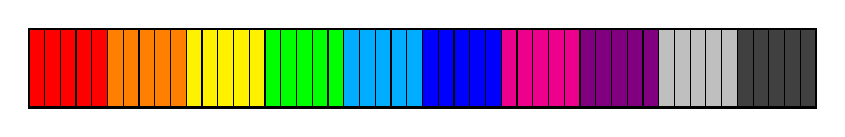
\begin{tikzpicture}
  \filldraw[fill=red]    (0, 0) rectangle  +(1,1);
  \filldraw[fill=orange] (1, 0) rectangle  +(1,1);
  \filldraw[fill=yellow] (2, 0) rectangle  +(1,1);
  \filldraw[fill=green]  (3, 0) rectangle  +(1,1);
  \filldraw[fill=cyan]   (4, 0) rectangle  +(1,1);
  \filldraw[fill=blue]   (5, 0) rectangle  +(1,1);
  \filldraw[fill=magenta] (6, 0) rectangle  +(1,1);
  \filldraw[fill=violet] (7, 0) rectangle +(1,1);
  \filldraw[fill=lightgray] (8, 0) rectangle +(1,1);
  \filldraw[fill=darkgray] (9, 0) rectangle +(1,1);
  
  \draw[thick] (0, 0) rectangle (10, 1);
  \foreach \i in {0.2, 0.4, ..., 9.8}
  \draw (\i, 0) -- +(0, 1);
\end{tikzpicture}

\bigskip

\begin{block}{$\texttt{reduce}(A, n):$}
  \begin{enumerate}
  \item Si $n = 1$, renvoyer $A[0]$.
  \item Allouer un tableau \texttt{Scratch} de taille $n/2$.
  \item Pour tout $0 \leq i < n/2$, faire (en parallèle):
    \begin{itemize}
    \item $\texttt{Scratch}[i] \gets A[2i] + A[2i+1]$.  
    \end{itemize}
    
  \item renvoyer : $\texttt{reduce}(\texttt{Scratch}, n/2)$.
  \end{enumerate}
\end{block}

\begin{align*}
  T &= \frac{2n}{p} + \log_2 p \\
    &\geq 1 + \log_2 p & \text{(optimal atteint avec $n/2$ processeurs)}
\end{align*}
\end{frame}





% Charles' emacs magic commands
%%% Local Variables:
%%% TeX-engine: xetex
%%% TeX-command-extra: "-shell-escape"
%%% TeX-command-extra-options: "-shell-escape"
%%% ispell-local-dictionary: "english"
%%% eval: (flyspell-mode 1)
%%% eval: (reftex-mode 1)
%%% End:
